% PREAMBLE

%\documentclass[a4paper,10pt,rmp,onecolumn,secnumarabic,numerical,balancelastpage,amsmath,amssymb,hyperref=pdftex,superscriptaddress]{article}

\documentclass[10pt,a4paper,aps,twocolumn,secnumarabic,numerical,balancelastpage,nofootinbib,superscriptaddress]{revtex4-2}

\usepackage[T1]{fontenc} % Vise norske tegn
\usepackage{ulem} % for \uuline (double underline)
\usepackage[utf8]{inputenc} % For å kunne skrive norske tegn
\usepackage{babel} % Tilpasning til norsk
\usepackage{graphicx} % For å inkludere grafikk
\usepackage{epstopdf}
%\usepackage{caption}
\usepackage{subcaption}
\usepackage{bbm}
%\captionsetup[figure]{name=Figure}
\usepackage{amsmath,amssymb, mathtools} % Ekstra matematikkfunksjoner
\usepackage[dvips,a4paper,margin=2.5cm,bottom=1.5cm]{geometry}
\usepackage{physics} % Use the physics package
\usepackage{dcolumn}% Align table columns on decimal point
\usepackage{geometry} % Required for adjusting page dimensions and margins
\usepackage{hyperref}
\hypersetup{
	colorlinks=true
}

\geometry{
	paper=a4paper, % Paper size, change to letterpaper for US letter size
	top=2.5cm, % Top margin
	bottom=2.5cm, % Bottom margin
	left=2.5cm, % Left margin
	right=2.5cm, % Right margin
	headheight=14pt, % Header height
	footskip=1.5cm, % Space from the bottom margin to the baseline of the footer
	headsep=1.2cm, % Space from the top margin to the baseline of the header
	%showframe, % Uncomment to show how the type block is set on the page
}
%\usepackage[backend=bibtex,style=authoryear,autocite=inline]{biblatex}

%\usepackage{authblk} % pakke for author visning
%\renewcommand\Authand{, og } % for å erstatte and med og i author
%\renewcommand\Authands{, og }

%\addbibresource{ref.bib}
%\addtolength\topmargin{-.5\topmargin} %cuts the top margin in half.
%\usepackage{geometry}
%\nocite{*}

\begin{document}

\preprint{APS/123-QED}

\title{Exploration of particles in confined spaces:\\using numerical methods}% Force line breaks with \\
%\thanks{A footnote to the article title}%

\author{Stian S. Johannessen}
 \homepage{https://folk.ntnu.no/stiansjo}
 \email{stiansjo@stud.ntnu.no}
 \affiliation{Department of Physics, NTNU, Norway.}
\date{\today}

\begin{abstract}
	The goal of this project is to explore numerically how gasses behave and how it might relate to statistical mechanics.
\end{abstract}

\maketitle

	\section{Method}
	
		The implementation of a verlet algorithm to simulate a two dimensional gas inside a rectangular box. Each particle has a position and velocity which is updated according to
		\begin{align}
			\va*{r}_i(t+\Delta t)&=\va*{r}_i(t)+\va*{v}_i(t)\Delta t+\frac{1}{2}\frac{\va*{f}_i(t)}{m}\Delta t^2\\
			\va*{v}_i(t+\Delta t)&=\va*{v}_i(t) +\frac{\va*{f}_i(t)+\va*{f}_i(t+\Delta t)}{2m}\Delta t
		\end{align}
		where the force
		\begin{align}
			\va*{f}_i&=-\pdv{V_w}{\va*{r}_i}-\sum_{j\neq i}\pdv{V(r_{ij})}{\va*{r}_i}
		\end{align}
		is given by the wall potential $V_w=V_x+V_y$ and the particle-particle potential $V(r_{ij})$
		\begin{align}
			V(r_{ij})&=\epsilon \left [\left (\frac{a}{r_{ij}}\right )^{12}-2\left (\frac{a}{r_{ij}}\right )^6\right ]\\
			V_x(\va*{r}_i)&=
			\begin{cases}
				\frac{K}{2}(x_i-L_x)^2	&	\text{if }x >L_x\\
				\frac{K}{2}x_i^2	&	\text{if }x < 0
			\end{cases}\\
			V_y(\va*{r}_i)&=
			\begin{cases}
				\frac{K}{2}(y_i-L_y)^2	&	\text{if }y >L_y\\
				\frac{K}{2}y_i^2	&	\text{if }y < 0
			\end{cases}
		\end{align}
		where $\epsilon$ is the interaction parameter for the particles, $L_x$ and $L_y$ are the side length of the box, $K$ is the parameter which determines the "softness" of the walls and $a$ is the point where the switch between repulsive and attractive force between particles change, if the distance between the two particles $r_{ij}=a$ then we can say the two particles touch, so $a$ can be seen as the diameter of the particles. In order to make implementation easier $a=1$. Now the force between particles is
		\begin{align}
			\pdv{V(r_{ij})}{\va*{r}_i}&=12\epsilon\left [-\left (\frac{1}{r_{ij}}\right )^{13}+\left (\frac{1}{r_{ij}}\right )^7\right ].
		\end{align}
		The force from the walls is
		\begin{align}
			\pdv{V_x(x_i)}{x_i}&=
			\begin{cases}
				K(x_i-L_x)	&	\text{if }x > L_x\\
				Kx_i	&	\text{if } x < 0
			\end{cases}
		\end{align}
		with the same in the $y$ direction. We also choose the mass $m=1$ so the force becomes equal to the acceleration. This is also done to simplify the implementation. The program is written in fortran and the different states and simulations are set by editing an input file, the results should be able to be recreated by using the same inputs.
	
	
	\section{one particle}
		In order to simulate a gas first the system must be calibrated to one particle. First we can run different simulations with different time-steps to see how the particles behave. The box size is $10\times10$, the time is set to 10.
	\begin{figure*}[htb]
		\centering
		\begin{subfigure}{.45\textwidth}
			\hspace*{-2.6cm}\scalebox{0.9}{% GNUPLOT: LaTeX picture with Postscript
\begingroup
  % Encoding inside the plot.  In the header of your document, this encoding
  % should to defined, e.g., by using
  % \usepackage[cp1252,<other encodings>]{inputenc}
  \inputencoding{cp1252}%
  \makeatletter
  \providecommand\color[2][]{%
    \GenericError{(gnuplot) \space\space\space\@spaces}{%
      Package color not loaded in conjunction with
      terminal option `colourtext'%
    }{See the gnuplot documentation for explanation.%
    }{Either use 'blacktext' in gnuplot or load the package
      color.sty in LaTeX.}%
    \renewcommand\color[2][]{}%
  }%
  \providecommand\includegraphics[2][]{%
    \GenericError{(gnuplot) \space\space\space\@spaces}{%
      Package graphicx or graphics not loaded%
    }{See the gnuplot documentation for explanation.%
    }{The gnuplot epslatex terminal needs graphicx.sty or graphics.sty.}%
    \renewcommand\includegraphics[2][]{}%
  }%
  \providecommand\rotatebox[2]{#2}%
  \@ifundefined{ifGPcolor}{%
    \newif\ifGPcolor
    \GPcolorfalse
  }{}%
  \@ifundefined{ifGPblacktext}{%
    \newif\ifGPblacktext
    \GPblacktexttrue
  }{}%
  % define a \g@addto@macro without @ in the name:
  \let\gplgaddtomacro\g@addto@macro
  % define empty templates for all commands taking text:
  \gdef\gplbacktext{}%
  \gdef\gplfronttext{}%
  \makeatother
  \ifGPblacktext
    % no textcolor at all
    \def\colorrgb#1{}%
    \def\colorgray#1{}%
  \else
    % gray or color?
    \ifGPcolor
      \def\colorrgb#1{\color[rgb]{#1}}%
      \def\colorgray#1{\color[gray]{#1}}%
      \expandafter\def\csname LTw\endcsname{\color{white}}%
      \expandafter\def\csname LTb\endcsname{\color{black}}%
      \expandafter\def\csname LTa\endcsname{\color{black}}%
      \expandafter\def\csname LT0\endcsname{\color[rgb]{1,0,0}}%
      \expandafter\def\csname LT1\endcsname{\color[rgb]{0,1,0}}%
      \expandafter\def\csname LT2\endcsname{\color[rgb]{0,0,1}}%
      \expandafter\def\csname LT3\endcsname{\color[rgb]{1,0,1}}%
      \expandafter\def\csname LT4\endcsname{\color[rgb]{0,1,1}}%
      \expandafter\def\csname LT5\endcsname{\color[rgb]{1,1,0}}%
      \expandafter\def\csname LT6\endcsname{\color[rgb]{0,0,0}}%
      \expandafter\def\csname LT7\endcsname{\color[rgb]{1,0.3,0}}%
      \expandafter\def\csname LT8\endcsname{\color[rgb]{0.5,0.5,0.5}}%
    \else
      % gray
      \def\colorrgb#1{\color{black}}%
      \def\colorgray#1{\color[gray]{#1}}%
      \expandafter\def\csname LTw\endcsname{\color{white}}%
      \expandafter\def\csname LTb\endcsname{\color{black}}%
      \expandafter\def\csname LTa\endcsname{\color{black}}%
      \expandafter\def\csname LT0\endcsname{\color{black}}%
      \expandafter\def\csname LT1\endcsname{\color{black}}%
      \expandafter\def\csname LT2\endcsname{\color{black}}%
      \expandafter\def\csname LT3\endcsname{\color{black}}%
      \expandafter\def\csname LT4\endcsname{\color{black}}%
      \expandafter\def\csname LT5\endcsname{\color{black}}%
      \expandafter\def\csname LT6\endcsname{\color{black}}%
      \expandafter\def\csname LT7\endcsname{\color{black}}%
      \expandafter\def\csname LT8\endcsname{\color{black}}%
    \fi
  \fi
    \setlength{\unitlength}{0.0500bp}%
    \ifx\gptboxheight\undefined%
      \newlength{\gptboxheight}%
      \newlength{\gptboxwidth}%
      \newsavebox{\gptboxtext}%
    \fi%
    \setlength{\fboxrule}{0.5pt}%
    \setlength{\fboxsep}{1pt}%
\begin{picture}(7200.00,5040.00)%
    \gplgaddtomacro\gplbacktext{%
      \csname LTb\endcsname%%
      \put(1927,704){\makebox(0,0)[r]{\strut{}$-2$}}%
      \put(1927,1229){\makebox(0,0)[r]{\strut{}$0$}}%
      \put(1927,1754){\makebox(0,0)[r]{\strut{}$2$}}%
      \put(1927,2279){\makebox(0,0)[r]{\strut{}$4$}}%
      \put(1927,2804){\makebox(0,0)[r]{\strut{}$6$}}%
      \put(1927,3329){\makebox(0,0)[r]{\strut{}$8$}}%
      \put(1927,3854){\makebox(0,0)[r]{\strut{}$10$}}%
      \put(1927,4379){\makebox(0,0)[r]{\strut{}$12$}}%
      \put(2059,484){\makebox(0,0){\strut{}$-2$}}%
      \put(2584,484){\makebox(0,0){\strut{}$0$}}%
      \put(3109,484){\makebox(0,0){\strut{}$2$}}%
      \put(3634,484){\makebox(0,0){\strut{}$4$}}%
      \put(4159,484){\makebox(0,0){\strut{}$6$}}%
      \put(4684,484){\makebox(0,0){\strut{}$8$}}%
      \put(5209,484){\makebox(0,0){\strut{}$10$}}%
      \put(5734,484){\makebox(0,0){\strut{}$12$}}%
    }%
    \gplgaddtomacro\gplfronttext{%
      \csname LTb\endcsname%%
      \put(1465,2541){\makebox(0,0){\strut{}y}}%
      \put(3896,154){\makebox(0,0){\strut{}x}}%
      \put(3896,4709){\makebox(0,0){\strut{}Trajectory of 1 particle with $\Delta t = 0.001$}}%
      \csname LTb\endcsname%%
      \put(4747,4206){\makebox(0,0)[r]{\strut{}Trajectory}}%
    }%
    \gplbacktext
    \put(0,0){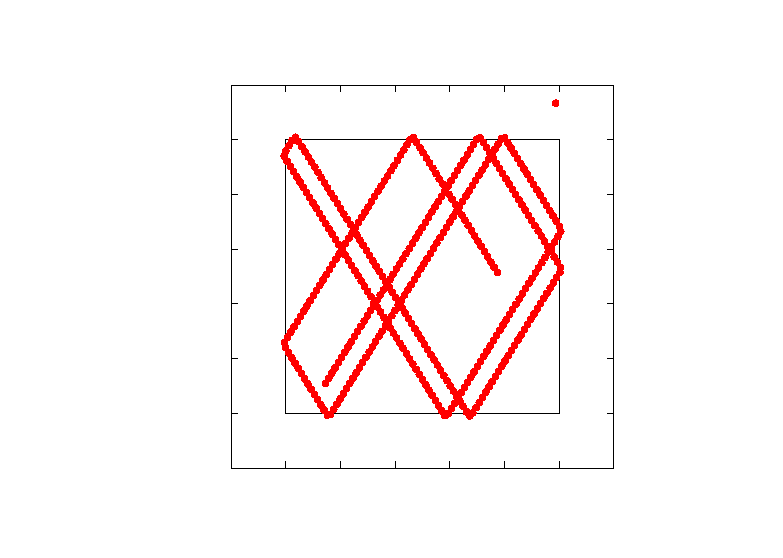
\includegraphics{../Report/figures/P_001_0001}}%
    \gplfronttext
  \end{picture}%
\endgroup
}
			\caption{Path of one particle with $\Delta t=0.001$}
		\end{subfigure}
		\begin{subfigure}{.45\textwidth}
			\hspace*{-2.6cm}\scalebox{0.9}{% GNUPLOT: LaTeX picture with Postscript
\begingroup
  % Encoding inside the plot.  In the header of your document, this encoding
  % should to defined, e.g., by using
  % \usepackage[cp1252,<other encodings>]{inputenc}
  \inputencoding{cp1252}%
  \makeatletter
  \providecommand\color[2][]{%
    \GenericError{(gnuplot) \space\space\space\@spaces}{%
      Package color not loaded in conjunction with
      terminal option `colourtext'%
    }{See the gnuplot documentation for explanation.%
    }{Either use 'blacktext' in gnuplot or load the package
      color.sty in LaTeX.}%
    \renewcommand\color[2][]{}%
  }%
  \providecommand\includegraphics[2][]{%
    \GenericError{(gnuplot) \space\space\space\@spaces}{%
      Package graphicx or graphics not loaded%
    }{See the gnuplot documentation for explanation.%
    }{The gnuplot epslatex terminal needs graphicx.sty or graphics.sty.}%
    \renewcommand\includegraphics[2][]{}%
  }%
  \providecommand\rotatebox[2]{#2}%
  \@ifundefined{ifGPcolor}{%
    \newif\ifGPcolor
    \GPcolortrue
  }{}%
  \@ifundefined{ifGPblacktext}{%
    \newif\ifGPblacktext
    \GPblacktexttrue
  }{}%
  % define a \g@addto@macro without @ in the name:
  \let\gplgaddtomacro\g@addto@macro
  % define empty templates for all commands taking text:
  \gdef\gplbacktext{}%
  \gdef\gplfronttext{}%
  \makeatother
  \ifGPblacktext
    % no textcolor at all
    \def\colorrgb#1{}%
    \def\colorgray#1{}%
  \else
    % gray or color?
    \ifGPcolor
      \def\colorrgb#1{\color[rgb]{#1}}%
      \def\colorgray#1{\color[gray]{#1}}%
      \expandafter\def\csname LTw\endcsname{\color{white}}%
      \expandafter\def\csname LTb\endcsname{\color{black}}%
      \expandafter\def\csname LTa\endcsname{\color{black}}%
      \expandafter\def\csname LT0\endcsname{\color[rgb]{1,0,0}}%
      \expandafter\def\csname LT1\endcsname{\color[rgb]{0,1,0}}%
      \expandafter\def\csname LT2\endcsname{\color[rgb]{0,0,1}}%
      \expandafter\def\csname LT3\endcsname{\color[rgb]{1,0,1}}%
      \expandafter\def\csname LT4\endcsname{\color[rgb]{0,1,1}}%
      \expandafter\def\csname LT5\endcsname{\color[rgb]{1,1,0}}%
      \expandafter\def\csname LT6\endcsname{\color[rgb]{0,0,0}}%
      \expandafter\def\csname LT7\endcsname{\color[rgb]{1,0.3,0}}%
      \expandafter\def\csname LT8\endcsname{\color[rgb]{0.5,0.5,0.5}}%
    \else
      % gray
      \def\colorrgb#1{\color{black}}%
      \def\colorgray#1{\color[gray]{#1}}%
      \expandafter\def\csname LTw\endcsname{\color{white}}%
      \expandafter\def\csname LTb\endcsname{\color{black}}%
      \expandafter\def\csname LTa\endcsname{\color{black}}%
      \expandafter\def\csname LT0\endcsname{\color{black}}%
      \expandafter\def\csname LT1\endcsname{\color{black}}%
      \expandafter\def\csname LT2\endcsname{\color{black}}%
      \expandafter\def\csname LT3\endcsname{\color{black}}%
      \expandafter\def\csname LT4\endcsname{\color{black}}%
      \expandafter\def\csname LT5\endcsname{\color{black}}%
      \expandafter\def\csname LT6\endcsname{\color{black}}%
      \expandafter\def\csname LT7\endcsname{\color{black}}%
      \expandafter\def\csname LT8\endcsname{\color{black}}%
    \fi
  \fi
    \setlength{\unitlength}{0.0500bp}%
    \ifx\gptboxheight\undefined%
      \newlength{\gptboxheight}%
      \newlength{\gptboxwidth}%
      \newsavebox{\gptboxtext}%
    \fi%
    \setlength{\fboxrule}{0.5pt}%
    \setlength{\fboxsep}{1pt}%
\begin{picture}(7200.00,5040.00)%
    \gplgaddtomacro\gplbacktext{%
      \csname LTb\endcsname%%
      \put(1927,704){\makebox(0,0)[r]{\strut{}$-2$}}%
      \put(1927,1229){\makebox(0,0)[r]{\strut{}$0$}}%
      \put(1927,1754){\makebox(0,0)[r]{\strut{}$2$}}%
      \put(1927,2279){\makebox(0,0)[r]{\strut{}$4$}}%
      \put(1927,2804){\makebox(0,0)[r]{\strut{}$6$}}%
      \put(1927,3329){\makebox(0,0)[r]{\strut{}$8$}}%
      \put(1927,3854){\makebox(0,0)[r]{\strut{}$10$}}%
      \put(1927,4379){\makebox(0,0)[r]{\strut{}$12$}}%
      \put(2059,484){\makebox(0,0){\strut{}$-2$}}%
      \put(2584,484){\makebox(0,0){\strut{}$0$}}%
      \put(3109,484){\makebox(0,0){\strut{}$2$}}%
      \put(3634,484){\makebox(0,0){\strut{}$4$}}%
      \put(4159,484){\makebox(0,0){\strut{}$6$}}%
      \put(4684,484){\makebox(0,0){\strut{}$8$}}%
      \put(5209,484){\makebox(0,0){\strut{}$10$}}%
      \put(5734,484){\makebox(0,0){\strut{}$12$}}%
    }%
    \gplgaddtomacro\gplfronttext{%
      \csname LTb\endcsname%%
      \put(1465,2541){\makebox(0,0){\strut{}y}}%
      \put(3896,154){\makebox(0,0){\strut{}x}}%
      \put(3896,4709){\makebox(0,0){\strut{}Trajectory of 1 particle with $\Delta t = 0.005$}}%
      \csname LTb\endcsname%%
      \put(4747,4206){\makebox(0,0)[r]{\strut{}Trajectory}}%
    }%
    \gplbacktext
    \put(0,0){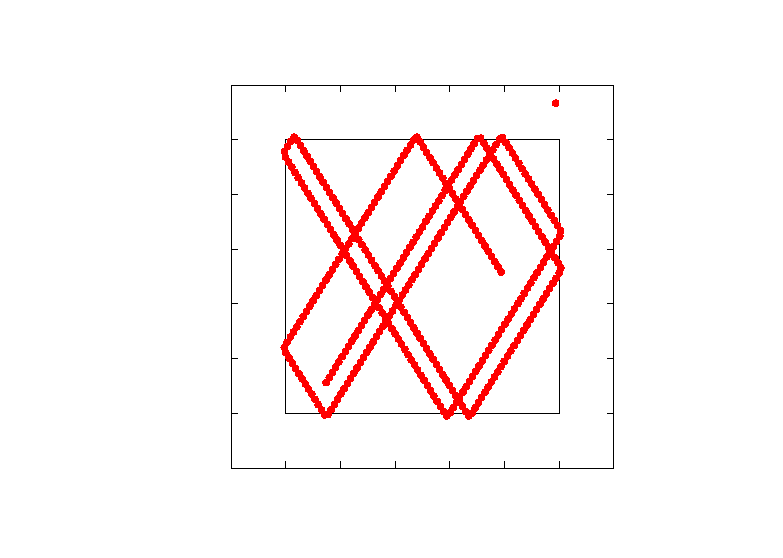
\includegraphics{../Report/figures/P_001_0005}}%
    \gplfronttext
  \end{picture}%
\endgroup
}
			\caption{Path of one particle with $\Delta t=0.005$}
		\end{subfigure}
		\begin{subfigure}{.45\textwidth}
			\hspace*{-2.6cm}\scalebox{0.9}{% GNUPLOT: LaTeX picture with Postscript
\begingroup
  % Encoding inside the plot.  In the header of your document, this encoding
  % should to defined, e.g., by using
  % \usepackage[cp1252,<other encodings>]{inputenc}
  \inputencoding{cp1252}%
  \makeatletter
  \providecommand\color[2][]{%
    \GenericError{(gnuplot) \space\space\space\@spaces}{%
      Package color not loaded in conjunction with
      terminal option `colourtext'%
    }{See the gnuplot documentation for explanation.%
    }{Either use 'blacktext' in gnuplot or load the package
      color.sty in LaTeX.}%
    \renewcommand\color[2][]{}%
  }%
  \providecommand\includegraphics[2][]{%
    \GenericError{(gnuplot) \space\space\space\@spaces}{%
      Package graphicx or graphics not loaded%
    }{See the gnuplot documentation for explanation.%
    }{The gnuplot epslatex terminal needs graphicx.sty or graphics.sty.}%
    \renewcommand\includegraphics[2][]{}%
  }%
  \providecommand\rotatebox[2]{#2}%
  \@ifundefined{ifGPcolor}{%
    \newif\ifGPcolor
    \GPcolortrue
  }{}%
  \@ifundefined{ifGPblacktext}{%
    \newif\ifGPblacktext
    \GPblacktexttrue
  }{}%
  % define a \g@addto@macro without @ in the name:
  \let\gplgaddtomacro\g@addto@macro
  % define empty templates for all commands taking text:
  \gdef\gplbacktext{}%
  \gdef\gplfronttext{}%
  \makeatother
  \ifGPblacktext
    % no textcolor at all
    \def\colorrgb#1{}%
    \def\colorgray#1{}%
  \else
    % gray or color?
    \ifGPcolor
      \def\colorrgb#1{\color[rgb]{#1}}%
      \def\colorgray#1{\color[gray]{#1}}%
      \expandafter\def\csname LTw\endcsname{\color{white}}%
      \expandafter\def\csname LTb\endcsname{\color{black}}%
      \expandafter\def\csname LTa\endcsname{\color{black}}%
      \expandafter\def\csname LT0\endcsname{\color[rgb]{1,0,0}}%
      \expandafter\def\csname LT1\endcsname{\color[rgb]{0,1,0}}%
      \expandafter\def\csname LT2\endcsname{\color[rgb]{0,0,1}}%
      \expandafter\def\csname LT3\endcsname{\color[rgb]{1,0,1}}%
      \expandafter\def\csname LT4\endcsname{\color[rgb]{0,1,1}}%
      \expandafter\def\csname LT5\endcsname{\color[rgb]{1,1,0}}%
      \expandafter\def\csname LT6\endcsname{\color[rgb]{0,0,0}}%
      \expandafter\def\csname LT7\endcsname{\color[rgb]{1,0.3,0}}%
      \expandafter\def\csname LT8\endcsname{\color[rgb]{0.5,0.5,0.5}}%
    \else
      % gray
      \def\colorrgb#1{\color{black}}%
      \def\colorgray#1{\color[gray]{#1}}%
      \expandafter\def\csname LTw\endcsname{\color{white}}%
      \expandafter\def\csname LTb\endcsname{\color{black}}%
      \expandafter\def\csname LTa\endcsname{\color{black}}%
      \expandafter\def\csname LT0\endcsname{\color{black}}%
      \expandafter\def\csname LT1\endcsname{\color{black}}%
      \expandafter\def\csname LT2\endcsname{\color{black}}%
      \expandafter\def\csname LT3\endcsname{\color{black}}%
      \expandafter\def\csname LT4\endcsname{\color{black}}%
      \expandafter\def\csname LT5\endcsname{\color{black}}%
      \expandafter\def\csname LT6\endcsname{\color{black}}%
      \expandafter\def\csname LT7\endcsname{\color{black}}%
      \expandafter\def\csname LT8\endcsname{\color{black}}%
    \fi
  \fi
    \setlength{\unitlength}{0.0500bp}%
    \ifx\gptboxheight\undefined%
      \newlength{\gptboxheight}%
      \newlength{\gptboxwidth}%
      \newsavebox{\gptboxtext}%
    \fi%
    \setlength{\fboxrule}{0.5pt}%
    \setlength{\fboxsep}{1pt}%
\begin{picture}(7200.00,5040.00)%
    \gplgaddtomacro\gplbacktext{%
      \csname LTb\endcsname%%
      \put(1927,704){\makebox(0,0)[r]{\strut{}$-2$}}%
      \put(1927,1229){\makebox(0,0)[r]{\strut{}$0$}}%
      \put(1927,1754){\makebox(0,0)[r]{\strut{}$2$}}%
      \put(1927,2279){\makebox(0,0)[r]{\strut{}$4$}}%
      \put(1927,2804){\makebox(0,0)[r]{\strut{}$6$}}%
      \put(1927,3329){\makebox(0,0)[r]{\strut{}$8$}}%
      \put(1927,3854){\makebox(0,0)[r]{\strut{}$10$}}%
      \put(1927,4379){\makebox(0,0)[r]{\strut{}$12$}}%
      \put(2059,484){\makebox(0,0){\strut{}$-2$}}%
      \put(2584,484){\makebox(0,0){\strut{}$0$}}%
      \put(3109,484){\makebox(0,0){\strut{}$2$}}%
      \put(3634,484){\makebox(0,0){\strut{}$4$}}%
      \put(4159,484){\makebox(0,0){\strut{}$6$}}%
      \put(4684,484){\makebox(0,0){\strut{}$8$}}%
      \put(5209,484){\makebox(0,0){\strut{}$10$}}%
      \put(5734,484){\makebox(0,0){\strut{}$12$}}%
    }%
    \gplgaddtomacro\gplfronttext{%
      \csname LTb\endcsname%%
      \put(1465,2541){\makebox(0,0){\strut{}y}}%
      \put(3896,154){\makebox(0,0){\strut{}x}}%
      \put(3896,4709){\makebox(0,0){\strut{}Trajectory of 1 particle with $\Delta t = 0.01$}}%
      \csname LTb\endcsname%%
      \put(4747,4206){\makebox(0,0)[r]{\strut{}Trajectory}}%
    }%
    \gplbacktext
    \put(0,0){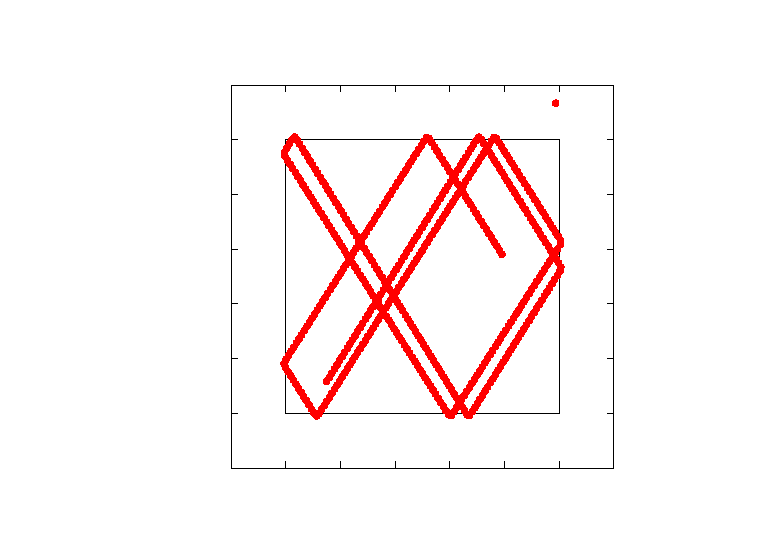
\includegraphics{../Report/figures/P_001_0010}}%
    \gplfronttext
  \end{picture}%
\endgroup
}
			\caption{Path of one particle with $\Delta t=0.01$}
		\end{subfigure}
		\begin{subfigure}{.45\textwidth}
			\hspace*{-2.6cm}\scalebox{0.9}{% GNUPLOT: LaTeX picture with Postscript
\begingroup
  % Encoding inside the plot.  In the header of your document, this encoding
  % should to defined, e.g., by using
  % \usepackage[cp1252,<other encodings>]{inputenc}
  \inputencoding{cp1252}%
  \makeatletter
  \providecommand\color[2][]{%
    \GenericError{(gnuplot) \space\space\space\@spaces}{%
      Package color not loaded in conjunction with
      terminal option `colourtext'%
    }{See the gnuplot documentation for explanation.%
    }{Either use 'blacktext' in gnuplot or load the package
      color.sty in LaTeX.}%
    \renewcommand\color[2][]{}%
  }%
  \providecommand\includegraphics[2][]{%
    \GenericError{(gnuplot) \space\space\space\@spaces}{%
      Package graphicx or graphics not loaded%
    }{See the gnuplot documentation for explanation.%
    }{The gnuplot epslatex terminal needs graphicx.sty or graphics.sty.}%
    \renewcommand\includegraphics[2][]{}%
  }%
  \providecommand\rotatebox[2]{#2}%
  \@ifundefined{ifGPcolor}{%
    \newif\ifGPcolor
    \GPcolortrue
  }{}%
  \@ifundefined{ifGPblacktext}{%
    \newif\ifGPblacktext
    \GPblacktexttrue
  }{}%
  % define a \g@addto@macro without @ in the name:
  \let\gplgaddtomacro\g@addto@macro
  % define empty templates for all commands taking text:
  \gdef\gplbacktext{}%
  \gdef\gplfronttext{}%
  \makeatother
  \ifGPblacktext
    % no textcolor at all
    \def\colorrgb#1{}%
    \def\colorgray#1{}%
  \else
    % gray or color?
    \ifGPcolor
      \def\colorrgb#1{\color[rgb]{#1}}%
      \def\colorgray#1{\color[gray]{#1}}%
      \expandafter\def\csname LTw\endcsname{\color{white}}%
      \expandafter\def\csname LTb\endcsname{\color{black}}%
      \expandafter\def\csname LTa\endcsname{\color{black}}%
      \expandafter\def\csname LT0\endcsname{\color[rgb]{1,0,0}}%
      \expandafter\def\csname LT1\endcsname{\color[rgb]{0,1,0}}%
      \expandafter\def\csname LT2\endcsname{\color[rgb]{0,0,1}}%
      \expandafter\def\csname LT3\endcsname{\color[rgb]{1,0,1}}%
      \expandafter\def\csname LT4\endcsname{\color[rgb]{0,1,1}}%
      \expandafter\def\csname LT5\endcsname{\color[rgb]{1,1,0}}%
      \expandafter\def\csname LT6\endcsname{\color[rgb]{0,0,0}}%
      \expandafter\def\csname LT7\endcsname{\color[rgb]{1,0.3,0}}%
      \expandafter\def\csname LT8\endcsname{\color[rgb]{0.5,0.5,0.5}}%
    \else
      % gray
      \def\colorrgb#1{\color{black}}%
      \def\colorgray#1{\color[gray]{#1}}%
      \expandafter\def\csname LTw\endcsname{\color{white}}%
      \expandafter\def\csname LTb\endcsname{\color{black}}%
      \expandafter\def\csname LTa\endcsname{\color{black}}%
      \expandafter\def\csname LT0\endcsname{\color{black}}%
      \expandafter\def\csname LT1\endcsname{\color{black}}%
      \expandafter\def\csname LT2\endcsname{\color{black}}%
      \expandafter\def\csname LT3\endcsname{\color{black}}%
      \expandafter\def\csname LT4\endcsname{\color{black}}%
      \expandafter\def\csname LT5\endcsname{\color{black}}%
      \expandafter\def\csname LT6\endcsname{\color{black}}%
      \expandafter\def\csname LT7\endcsname{\color{black}}%
      \expandafter\def\csname LT8\endcsname{\color{black}}%
    \fi
  \fi
    \setlength{\unitlength}{0.0500bp}%
    \ifx\gptboxheight\undefined%
      \newlength{\gptboxheight}%
      \newlength{\gptboxwidth}%
      \newsavebox{\gptboxtext}%
    \fi%
    \setlength{\fboxrule}{0.5pt}%
    \setlength{\fboxsep}{1pt}%
\begin{picture}(7200.00,5040.00)%
    \gplgaddtomacro\gplbacktext{%
      \csname LTb\endcsname%%
      \put(1927,704){\makebox(0,0)[r]{\strut{}$-2$}}%
      \put(1927,1229){\makebox(0,0)[r]{\strut{}$0$}}%
      \put(1927,1754){\makebox(0,0)[r]{\strut{}$2$}}%
      \put(1927,2279){\makebox(0,0)[r]{\strut{}$4$}}%
      \put(1927,2804){\makebox(0,0)[r]{\strut{}$6$}}%
      \put(1927,3329){\makebox(0,0)[r]{\strut{}$8$}}%
      \put(1927,3854){\makebox(0,0)[r]{\strut{}$10$}}%
      \put(1927,4379){\makebox(0,0)[r]{\strut{}$12$}}%
      \put(2059,484){\makebox(0,0){\strut{}$-2$}}%
      \put(2584,484){\makebox(0,0){\strut{}$0$}}%
      \put(3109,484){\makebox(0,0){\strut{}$2$}}%
      \put(3634,484){\makebox(0,0){\strut{}$4$}}%
      \put(4159,484){\makebox(0,0){\strut{}$6$}}%
      \put(4684,484){\makebox(0,0){\strut{}$8$}}%
      \put(5209,484){\makebox(0,0){\strut{}$10$}}%
      \put(5734,484){\makebox(0,0){\strut{}$12$}}%
    }%
    \gplgaddtomacro\gplfronttext{%
      \csname LTb\endcsname%%
      \put(1465,2541){\makebox(0,0){\strut{}y}}%
      \put(3896,154){\makebox(0,0){\strut{}x}}%
      \put(3896,4709){\makebox(0,0){\strut{}Trajectory of 1 particle with $\Delta t = 0.02$}}%
      \csname LTb\endcsname%%
      \put(4747,4206){\makebox(0,0)[r]{\strut{}Trajectory}}%
    }%
    \gplbacktext
    \put(0,0){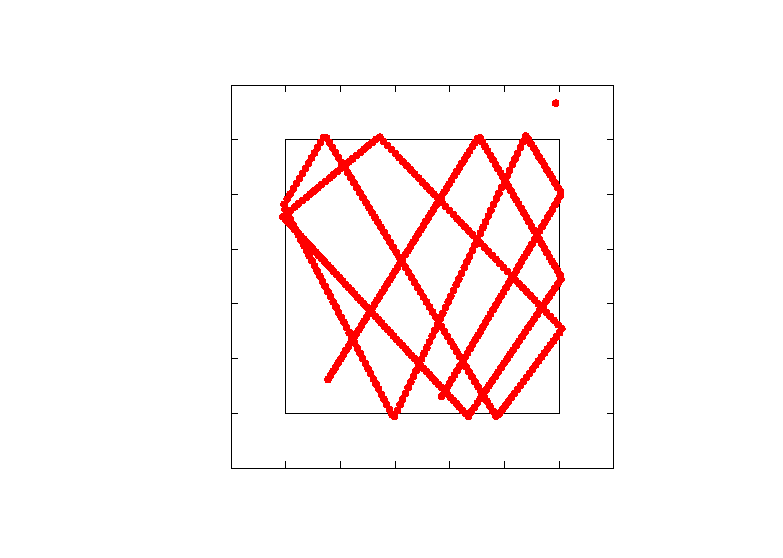
\includegraphics{../Report/figures/P_001_0020}}%
    \gplfronttext
  \end{picture}%
\endgroup
}
			\caption{Path of one particle with $\Delta t=0.02$}
		\end{subfigure}
		\caption{\label{fig:path}Path of one particle with different values of time step $\Delta t$ the wall constant $K=6000$}
	\end{figure*}
	In figure \ref{fig:path} the paths of 4 particles is traced over the same time but with different time steps, here we can see that a time step of $\Delta t = 0.01$ gives a decent trajectory. Time-steps above this results in a deteriorated path.
	\begin{figure*}[htb]
		\centering
		\begin{subfigure}{.45\textwidth}
			\scalebox{0.6}{% GNUPLOT: LaTeX picture with Postscript
\begingroup
  % Encoding inside the plot.  In the header of your document, this encoding
  % should to defined, e.g., by using
  % \usepackage[cp1252,<other encodings>]{inputenc}
  \inputencoding{cp1252}%
  \makeatletter
  \providecommand\color[2][]{%
    \GenericError{(gnuplot) \space\space\space\@spaces}{%
      Package color not loaded in conjunction with
      terminal option `colourtext'%
    }{See the gnuplot documentation for explanation.%
    }{Either use 'blacktext' in gnuplot or load the package
      color.sty in LaTeX.}%
    \renewcommand\color[2][]{}%
  }%
  \providecommand\includegraphics[2][]{%
    \GenericError{(gnuplot) \space\space\space\@spaces}{%
      Package graphicx or graphics not loaded%
    }{See the gnuplot documentation for explanation.%
    }{The gnuplot epslatex terminal needs graphicx.sty or graphics.sty.}%
    \renewcommand\includegraphics[2][]{}%
  }%
  \providecommand\rotatebox[2]{#2}%
  \@ifundefined{ifGPcolor}{%
    \newif\ifGPcolor
    \GPcolortrue
  }{}%
  \@ifundefined{ifGPblacktext}{%
    \newif\ifGPblacktext
    \GPblacktexttrue
  }{}%
  % define a \g@addto@macro without @ in the name:
  \let\gplgaddtomacro\g@addto@macro
  % define empty templates for all commands taking text:
  \gdef\gplbacktext{}%
  \gdef\gplfronttext{}%
  \makeatother
  \ifGPblacktext
    % no textcolor at all
    \def\colorrgb#1{}%
    \def\colorgray#1{}%
  \else
    % gray or color?
    \ifGPcolor
      \def\colorrgb#1{\color[rgb]{#1}}%
      \def\colorgray#1{\color[gray]{#1}}%
      \expandafter\def\csname LTw\endcsname{\color{white}}%
      \expandafter\def\csname LTb\endcsname{\color{black}}%
      \expandafter\def\csname LTa\endcsname{\color{black}}%
      \expandafter\def\csname LT0\endcsname{\color[rgb]{1,0,0}}%
      \expandafter\def\csname LT1\endcsname{\color[rgb]{0,1,0}}%
      \expandafter\def\csname LT2\endcsname{\color[rgb]{0,0,1}}%
      \expandafter\def\csname LT3\endcsname{\color[rgb]{1,0,1}}%
      \expandafter\def\csname LT4\endcsname{\color[rgb]{0,1,1}}%
      \expandafter\def\csname LT5\endcsname{\color[rgb]{1,1,0}}%
      \expandafter\def\csname LT6\endcsname{\color[rgb]{0,0,0}}%
      \expandafter\def\csname LT7\endcsname{\color[rgb]{1,0.3,0}}%
      \expandafter\def\csname LT8\endcsname{\color[rgb]{0.5,0.5,0.5}}%
    \else
      % gray
      \def\colorrgb#1{\color{black}}%
      \def\colorgray#1{\color[gray]{#1}}%
      \expandafter\def\csname LTw\endcsname{\color{white}}%
      \expandafter\def\csname LTb\endcsname{\color{black}}%
      \expandafter\def\csname LTa\endcsname{\color{black}}%
      \expandafter\def\csname LT0\endcsname{\color{black}}%
      \expandafter\def\csname LT1\endcsname{\color{black}}%
      \expandafter\def\csname LT2\endcsname{\color{black}}%
      \expandafter\def\csname LT3\endcsname{\color{black}}%
      \expandafter\def\csname LT4\endcsname{\color{black}}%
      \expandafter\def\csname LT5\endcsname{\color{black}}%
      \expandafter\def\csname LT6\endcsname{\color{black}}%
      \expandafter\def\csname LT7\endcsname{\color{black}}%
      \expandafter\def\csname LT8\endcsname{\color{black}}%
    \fi
  \fi
    \setlength{\unitlength}{0.0500bp}%
    \ifx\gptboxheight\undefined%
      \newlength{\gptboxheight}%
      \newlength{\gptboxwidth}%
      \newsavebox{\gptboxtext}%
    \fi%
    \setlength{\fboxrule}{0.5pt}%
    \setlength{\fboxsep}{1pt}%
\begin{picture}(7200.00,5040.00)%
    \gplgaddtomacro\gplbacktext{%
      \csname LTb\endcsname%%
      \put(858,704){\makebox(0,0)[r]{\strut{}$0$}}%
      \put(858,1439){\makebox(0,0)[r]{\strut{}$10$}}%
      \put(858,2174){\makebox(0,0)[r]{\strut{}$20$}}%
      \put(858,2909){\makebox(0,0)[r]{\strut{}$30$}}%
      \put(858,3644){\makebox(0,0)[r]{\strut{}$40$}}%
      \put(858,4379){\makebox(0,0)[r]{\strut{}$50$}}%
      \put(990,484){\makebox(0,0){\strut{}$0$}}%
      \put(1571,484){\makebox(0,0){\strut{}$1$}}%
      \put(2153,484){\makebox(0,0){\strut{}$2$}}%
      \put(2734,484){\makebox(0,0){\strut{}$3$}}%
      \put(3315,484){\makebox(0,0){\strut{}$4$}}%
      \put(3897,484){\makebox(0,0){\strut{}$5$}}%
      \put(4478,484){\makebox(0,0){\strut{}$6$}}%
      \put(5059,484){\makebox(0,0){\strut{}$7$}}%
      \put(5640,484){\makebox(0,0){\strut{}$8$}}%
      \put(6222,484){\makebox(0,0){\strut{}$9$}}%
      \put(6803,484){\makebox(0,0){\strut{}$10$}}%
    }%
    \gplgaddtomacro\gplfronttext{%
      \csname LTb\endcsname%%
      \put(396,2541){\makebox(0,0){\strut{}E}}%
      \put(3896,154){\makebox(0,0){\strut{}T}}%
      \put(3896,4709){\makebox(0,0){\strut{}Total energy of 1 particle with $\Delta t = 0.001$}}%
      \csname LTb\endcsname%%
      \put(5816,4206){\makebox(0,0)[r]{\strut{}Energy}}%
    }%
    \gplbacktext
    \put(0,0){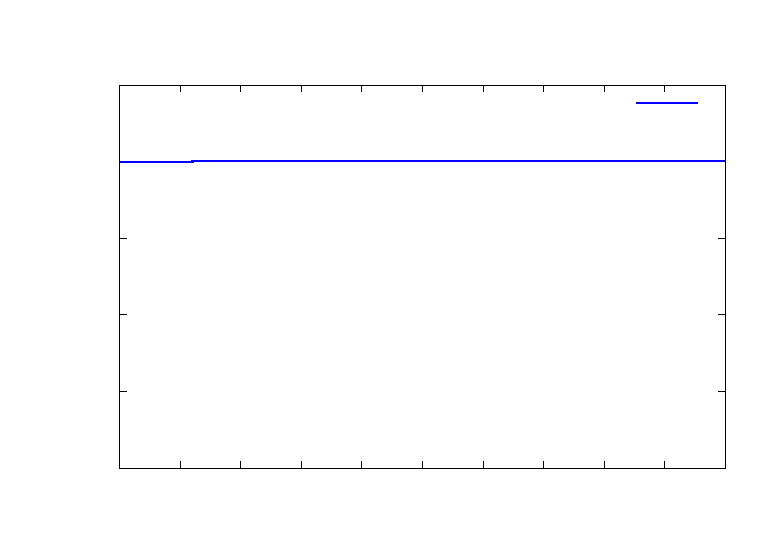
\includegraphics{../Report/figures/E_001_0001}}%
    \gplfronttext
  \end{picture}%
\endgroup
}
			\caption{Energy drift of one particle with $\Delta t=0.001$}
		\end{subfigure}
		\begin{subfigure}{.45\textwidth}
			\scalebox{0.6}{% GNUPLOT: LaTeX picture with Postscript
\begingroup
  % Encoding inside the plot.  In the header of your document, this encoding
  % should to defined, e.g., by using
  % \usepackage[cp1252,<other encodings>]{inputenc}
  \inputencoding{cp1252}%
  \makeatletter
  \providecommand\color[2][]{%
    \GenericError{(gnuplot) \space\space\space\@spaces}{%
      Package color not loaded in conjunction with
      terminal option `colourtext'%
    }{See the gnuplot documentation for explanation.%
    }{Either use 'blacktext' in gnuplot or load the package
      color.sty in LaTeX.}%
    \renewcommand\color[2][]{}%
  }%
  \providecommand\includegraphics[2][]{%
    \GenericError{(gnuplot) \space\space\space\@spaces}{%
      Package graphicx or graphics not loaded%
    }{See the gnuplot documentation for explanation.%
    }{The gnuplot epslatex terminal needs graphicx.sty or graphics.sty.}%
    \renewcommand\includegraphics[2][]{}%
  }%
  \providecommand\rotatebox[2]{#2}%
  \@ifundefined{ifGPcolor}{%
    \newif\ifGPcolor
    \GPcolortrue
  }{}%
  \@ifundefined{ifGPblacktext}{%
    \newif\ifGPblacktext
    \GPblacktexttrue
  }{}%
  % define a \g@addto@macro without @ in the name:
  \let\gplgaddtomacro\g@addto@macro
  % define empty templates for all commands taking text:
  \gdef\gplbacktext{}%
  \gdef\gplfronttext{}%
  \makeatother
  \ifGPblacktext
    % no textcolor at all
    \def\colorrgb#1{}%
    \def\colorgray#1{}%
  \else
    % gray or color?
    \ifGPcolor
      \def\colorrgb#1{\color[rgb]{#1}}%
      \def\colorgray#1{\color[gray]{#1}}%
      \expandafter\def\csname LTw\endcsname{\color{white}}%
      \expandafter\def\csname LTb\endcsname{\color{black}}%
      \expandafter\def\csname LTa\endcsname{\color{black}}%
      \expandafter\def\csname LT0\endcsname{\color[rgb]{1,0,0}}%
      \expandafter\def\csname LT1\endcsname{\color[rgb]{0,1,0}}%
      \expandafter\def\csname LT2\endcsname{\color[rgb]{0,0,1}}%
      \expandafter\def\csname LT3\endcsname{\color[rgb]{1,0,1}}%
      \expandafter\def\csname LT4\endcsname{\color[rgb]{0,1,1}}%
      \expandafter\def\csname LT5\endcsname{\color[rgb]{1,1,0}}%
      \expandafter\def\csname LT6\endcsname{\color[rgb]{0,0,0}}%
      \expandafter\def\csname LT7\endcsname{\color[rgb]{1,0.3,0}}%
      \expandafter\def\csname LT8\endcsname{\color[rgb]{0.5,0.5,0.5}}%
    \else
      % gray
      \def\colorrgb#1{\color{black}}%
      \def\colorgray#1{\color[gray]{#1}}%
      \expandafter\def\csname LTw\endcsname{\color{white}}%
      \expandafter\def\csname LTb\endcsname{\color{black}}%
      \expandafter\def\csname LTa\endcsname{\color{black}}%
      \expandafter\def\csname LT0\endcsname{\color{black}}%
      \expandafter\def\csname LT1\endcsname{\color{black}}%
      \expandafter\def\csname LT2\endcsname{\color{black}}%
      \expandafter\def\csname LT3\endcsname{\color{black}}%
      \expandafter\def\csname LT4\endcsname{\color{black}}%
      \expandafter\def\csname LT5\endcsname{\color{black}}%
      \expandafter\def\csname LT6\endcsname{\color{black}}%
      \expandafter\def\csname LT7\endcsname{\color{black}}%
      \expandafter\def\csname LT8\endcsname{\color{black}}%
    \fi
  \fi
    \setlength{\unitlength}{0.0500bp}%
    \ifx\gptboxheight\undefined%
      \newlength{\gptboxheight}%
      \newlength{\gptboxwidth}%
      \newsavebox{\gptboxtext}%
    \fi%
    \setlength{\fboxrule}{0.5pt}%
    \setlength{\fboxsep}{1pt}%
\begin{picture}(7200.00,5040.00)%
    \gplgaddtomacro\gplbacktext{%
      \csname LTb\endcsname%%
      \put(858,704){\makebox(0,0)[r]{\strut{}$0$}}%
      \put(858,1439){\makebox(0,0)[r]{\strut{}$10$}}%
      \put(858,2174){\makebox(0,0)[r]{\strut{}$20$}}%
      \put(858,2909){\makebox(0,0)[r]{\strut{}$30$}}%
      \put(858,3644){\makebox(0,0)[r]{\strut{}$40$}}%
      \put(858,4379){\makebox(0,0)[r]{\strut{}$50$}}%
      \put(990,484){\makebox(0,0){\strut{}$0$}}%
      \put(1571,484){\makebox(0,0){\strut{}$1$}}%
      \put(2153,484){\makebox(0,0){\strut{}$2$}}%
      \put(2734,484){\makebox(0,0){\strut{}$3$}}%
      \put(3315,484){\makebox(0,0){\strut{}$4$}}%
      \put(3897,484){\makebox(0,0){\strut{}$5$}}%
      \put(4478,484){\makebox(0,0){\strut{}$6$}}%
      \put(5059,484){\makebox(0,0){\strut{}$7$}}%
      \put(5640,484){\makebox(0,0){\strut{}$8$}}%
      \put(6222,484){\makebox(0,0){\strut{}$9$}}%
      \put(6803,484){\makebox(0,0){\strut{}$10$}}%
    }%
    \gplgaddtomacro\gplfronttext{%
      \csname LTb\endcsname%%
      \put(396,2541){\makebox(0,0){\strut{}E}}%
      \put(3896,154){\makebox(0,0){\strut{}T}}%
      \put(3896,4709){\makebox(0,0){\strut{}Total energy of 1 particle with $\Delta t = 0.005$}}%
      \csname LTb\endcsname%%
      \put(5816,4206){\makebox(0,0)[r]{\strut{}Energy}}%
    }%
    \gplbacktext
    \put(0,0){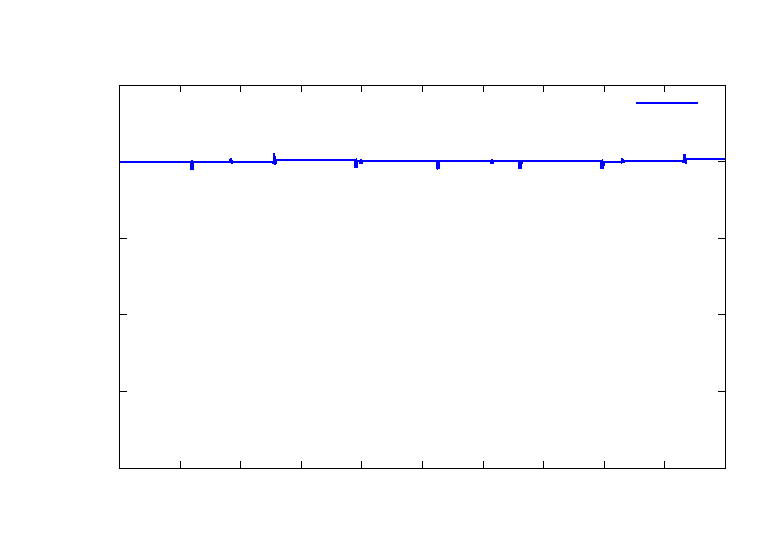
\includegraphics{../Report/figures/E_001_0005}}%
    \gplfronttext
  \end{picture}%
\endgroup
}
			\caption{Energy drift of one particle with $\Delta t=0.005$}
		\end{subfigure}
		\begin{subfigure}{.45\textwidth}
			\scalebox{0.6}{% GNUPLOT: LaTeX picture with Postscript
\begingroup
  % Encoding inside the plot.  In the header of your document, this encoding
  % should to defined, e.g., by using
  % \usepackage[cp1252,<other encodings>]{inputenc}
  \inputencoding{cp1252}%
  \makeatletter
  \providecommand\color[2][]{%
    \GenericError{(gnuplot) \space\space\space\@spaces}{%
      Package color not loaded in conjunction with
      terminal option `colourtext'%
    }{See the gnuplot documentation for explanation.%
    }{Either use 'blacktext' in gnuplot or load the package
      color.sty in LaTeX.}%
    \renewcommand\color[2][]{}%
  }%
  \providecommand\includegraphics[2][]{%
    \GenericError{(gnuplot) \space\space\space\@spaces}{%
      Package graphicx or graphics not loaded%
    }{See the gnuplot documentation for explanation.%
    }{The gnuplot epslatex terminal needs graphicx.sty or graphics.sty.}%
    \renewcommand\includegraphics[2][]{}%
  }%
  \providecommand\rotatebox[2]{#2}%
  \@ifundefined{ifGPcolor}{%
    \newif\ifGPcolor
    \GPcolortrue
  }{}%
  \@ifundefined{ifGPblacktext}{%
    \newif\ifGPblacktext
    \GPblacktexttrue
  }{}%
  % define a \g@addto@macro without @ in the name:
  \let\gplgaddtomacro\g@addto@macro
  % define empty templates for all commands taking text:
  \gdef\gplbacktext{}%
  \gdef\gplfronttext{}%
  \makeatother
  \ifGPblacktext
    % no textcolor at all
    \def\colorrgb#1{}%
    \def\colorgray#1{}%
  \else
    % gray or color?
    \ifGPcolor
      \def\colorrgb#1{\color[rgb]{#1}}%
      \def\colorgray#1{\color[gray]{#1}}%
      \expandafter\def\csname LTw\endcsname{\color{white}}%
      \expandafter\def\csname LTb\endcsname{\color{black}}%
      \expandafter\def\csname LTa\endcsname{\color{black}}%
      \expandafter\def\csname LT0\endcsname{\color[rgb]{1,0,0}}%
      \expandafter\def\csname LT1\endcsname{\color[rgb]{0,1,0}}%
      \expandafter\def\csname LT2\endcsname{\color[rgb]{0,0,1}}%
      \expandafter\def\csname LT3\endcsname{\color[rgb]{1,0,1}}%
      \expandafter\def\csname LT4\endcsname{\color[rgb]{0,1,1}}%
      \expandafter\def\csname LT5\endcsname{\color[rgb]{1,1,0}}%
      \expandafter\def\csname LT6\endcsname{\color[rgb]{0,0,0}}%
      \expandafter\def\csname LT7\endcsname{\color[rgb]{1,0.3,0}}%
      \expandafter\def\csname LT8\endcsname{\color[rgb]{0.5,0.5,0.5}}%
    \else
      % gray
      \def\colorrgb#1{\color{black}}%
      \def\colorgray#1{\color[gray]{#1}}%
      \expandafter\def\csname LTw\endcsname{\color{white}}%
      \expandafter\def\csname LTb\endcsname{\color{black}}%
      \expandafter\def\csname LTa\endcsname{\color{black}}%
      \expandafter\def\csname LT0\endcsname{\color{black}}%
      \expandafter\def\csname LT1\endcsname{\color{black}}%
      \expandafter\def\csname LT2\endcsname{\color{black}}%
      \expandafter\def\csname LT3\endcsname{\color{black}}%
      \expandafter\def\csname LT4\endcsname{\color{black}}%
      \expandafter\def\csname LT5\endcsname{\color{black}}%
      \expandafter\def\csname LT6\endcsname{\color{black}}%
      \expandafter\def\csname LT7\endcsname{\color{black}}%
      \expandafter\def\csname LT8\endcsname{\color{black}}%
    \fi
  \fi
    \setlength{\unitlength}{0.0500bp}%
    \ifx\gptboxheight\undefined%
      \newlength{\gptboxheight}%
      \newlength{\gptboxwidth}%
      \newsavebox{\gptboxtext}%
    \fi%
    \setlength{\fboxrule}{0.5pt}%
    \setlength{\fboxsep}{1pt}%
\begin{picture}(7200.00,5040.00)%
    \gplgaddtomacro\gplbacktext{%
      \csname LTb\endcsname%%
      \put(858,704){\makebox(0,0)[r]{\strut{}$0$}}%
      \put(858,1439){\makebox(0,0)[r]{\strut{}$10$}}%
      \put(858,2174){\makebox(0,0)[r]{\strut{}$20$}}%
      \put(858,2909){\makebox(0,0)[r]{\strut{}$30$}}%
      \put(858,3644){\makebox(0,0)[r]{\strut{}$40$}}%
      \put(858,4379){\makebox(0,0)[r]{\strut{}$50$}}%
      \put(990,484){\makebox(0,0){\strut{}$0$}}%
      \put(1571,484){\makebox(0,0){\strut{}$1$}}%
      \put(2153,484){\makebox(0,0){\strut{}$2$}}%
      \put(2734,484){\makebox(0,0){\strut{}$3$}}%
      \put(3315,484){\makebox(0,0){\strut{}$4$}}%
      \put(3897,484){\makebox(0,0){\strut{}$5$}}%
      \put(4478,484){\makebox(0,0){\strut{}$6$}}%
      \put(5059,484){\makebox(0,0){\strut{}$7$}}%
      \put(5640,484){\makebox(0,0){\strut{}$8$}}%
      \put(6222,484){\makebox(0,0){\strut{}$9$}}%
      \put(6803,484){\makebox(0,0){\strut{}$10$}}%
    }%
    \gplgaddtomacro\gplfronttext{%
      \csname LTb\endcsname%%
      \put(396,2541){\makebox(0,0){\strut{}E}}%
      \put(3896,154){\makebox(0,0){\strut{}T}}%
      \put(3896,4709){\makebox(0,0){\strut{}Total energy of 1 particle with $\Delta t = 0.01$}}%
      \csname LTb\endcsname%%
      \put(5816,4206){\makebox(0,0)[r]{\strut{}Energy}}%
    }%
    \gplbacktext
    \put(0,0){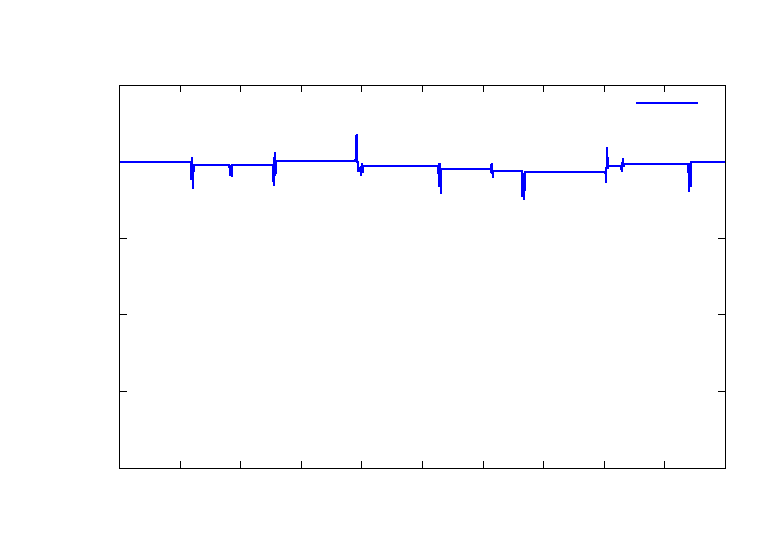
\includegraphics{../Report/figures/E_001_0010}}%
    \gplfronttext
  \end{picture}%
\endgroup
}
			\caption{Energy drift of one particle with $\Delta t=0.01$}
		\end{subfigure}
		\begin{subfigure}{.45\textwidth}
			\scalebox{0.6}{% GNUPLOT: LaTeX picture with Postscript
\begingroup
  % Encoding inside the plot.  In the header of your document, this encoding
  % should to defined, e.g., by using
  % \usepackage[cp1252,<other encodings>]{inputenc}
  \inputencoding{cp1252}%
  \makeatletter
  \providecommand\color[2][]{%
    \GenericError{(gnuplot) \space\space\space\@spaces}{%
      Package color not loaded in conjunction with
      terminal option `colourtext'%
    }{See the gnuplot documentation for explanation.%
    }{Either use 'blacktext' in gnuplot or load the package
      color.sty in LaTeX.}%
    \renewcommand\color[2][]{}%
  }%
  \providecommand\includegraphics[2][]{%
    \GenericError{(gnuplot) \space\space\space\@spaces}{%
      Package graphicx or graphics not loaded%
    }{See the gnuplot documentation for explanation.%
    }{The gnuplot epslatex terminal needs graphicx.sty or graphics.sty.}%
    \renewcommand\includegraphics[2][]{}%
  }%
  \providecommand\rotatebox[2]{#2}%
  \@ifundefined{ifGPcolor}{%
    \newif\ifGPcolor
    \GPcolortrue
  }{}%
  \@ifundefined{ifGPblacktext}{%
    \newif\ifGPblacktext
    \GPblacktexttrue
  }{}%
  % define a \g@addto@macro without @ in the name:
  \let\gplgaddtomacro\g@addto@macro
  % define empty templates for all commands taking text:
  \gdef\gplbacktext{}%
  \gdef\gplfronttext{}%
  \makeatother
  \ifGPblacktext
    % no textcolor at all
    \def\colorrgb#1{}%
    \def\colorgray#1{}%
  \else
    % gray or color?
    \ifGPcolor
      \def\colorrgb#1{\color[rgb]{#1}}%
      \def\colorgray#1{\color[gray]{#1}}%
      \expandafter\def\csname LTw\endcsname{\color{white}}%
      \expandafter\def\csname LTb\endcsname{\color{black}}%
      \expandafter\def\csname LTa\endcsname{\color{black}}%
      \expandafter\def\csname LT0\endcsname{\color[rgb]{1,0,0}}%
      \expandafter\def\csname LT1\endcsname{\color[rgb]{0,1,0}}%
      \expandafter\def\csname LT2\endcsname{\color[rgb]{0,0,1}}%
      \expandafter\def\csname LT3\endcsname{\color[rgb]{1,0,1}}%
      \expandafter\def\csname LT4\endcsname{\color[rgb]{0,1,1}}%
      \expandafter\def\csname LT5\endcsname{\color[rgb]{1,1,0}}%
      \expandafter\def\csname LT6\endcsname{\color[rgb]{0,0,0}}%
      \expandafter\def\csname LT7\endcsname{\color[rgb]{1,0.3,0}}%
      \expandafter\def\csname LT8\endcsname{\color[rgb]{0.5,0.5,0.5}}%
    \else
      % gray
      \def\colorrgb#1{\color{black}}%
      \def\colorgray#1{\color[gray]{#1}}%
      \expandafter\def\csname LTw\endcsname{\color{white}}%
      \expandafter\def\csname LTb\endcsname{\color{black}}%
      \expandafter\def\csname LTa\endcsname{\color{black}}%
      \expandafter\def\csname LT0\endcsname{\color{black}}%
      \expandafter\def\csname LT1\endcsname{\color{black}}%
      \expandafter\def\csname LT2\endcsname{\color{black}}%
      \expandafter\def\csname LT3\endcsname{\color{black}}%
      \expandafter\def\csname LT4\endcsname{\color{black}}%
      \expandafter\def\csname LT5\endcsname{\color{black}}%
      \expandafter\def\csname LT6\endcsname{\color{black}}%
      \expandafter\def\csname LT7\endcsname{\color{black}}%
      \expandafter\def\csname LT8\endcsname{\color{black}}%
    \fi
  \fi
    \setlength{\unitlength}{0.0500bp}%
    \ifx\gptboxheight\undefined%
      \newlength{\gptboxheight}%
      \newlength{\gptboxwidth}%
      \newsavebox{\gptboxtext}%
    \fi%
    \setlength{\fboxrule}{0.5pt}%
    \setlength{\fboxsep}{1pt}%
\begin{picture}(7200.00,5040.00)%
    \gplgaddtomacro\gplbacktext{%
      \csname LTb\endcsname%%
      \put(858,704){\makebox(0,0)[r]{\strut{}$0$}}%
      \put(858,1163){\makebox(0,0)[r]{\strut{}$10$}}%
      \put(858,1623){\makebox(0,0)[r]{\strut{}$20$}}%
      \put(858,2082){\makebox(0,0)[r]{\strut{}$30$}}%
      \put(858,2542){\makebox(0,0)[r]{\strut{}$40$}}%
      \put(858,3001){\makebox(0,0)[r]{\strut{}$50$}}%
      \put(858,3460){\makebox(0,0)[r]{\strut{}$60$}}%
      \put(858,3920){\makebox(0,0)[r]{\strut{}$70$}}%
      \put(858,4379){\makebox(0,0)[r]{\strut{}$80$}}%
      \put(990,484){\makebox(0,0){\strut{}$0$}}%
      \put(1571,484){\makebox(0,0){\strut{}$1$}}%
      \put(2153,484){\makebox(0,0){\strut{}$2$}}%
      \put(2734,484){\makebox(0,0){\strut{}$3$}}%
      \put(3315,484){\makebox(0,0){\strut{}$4$}}%
      \put(3897,484){\makebox(0,0){\strut{}$5$}}%
      \put(4478,484){\makebox(0,0){\strut{}$6$}}%
      \put(5059,484){\makebox(0,0){\strut{}$7$}}%
      \put(5640,484){\makebox(0,0){\strut{}$8$}}%
      \put(6222,484){\makebox(0,0){\strut{}$9$}}%
      \put(6803,484){\makebox(0,0){\strut{}$10$}}%
    }%
    \gplgaddtomacro\gplfronttext{%
      \csname LTb\endcsname%%
      \put(396,2541){\makebox(0,0){\strut{}E}}%
      \put(3896,154){\makebox(0,0){\strut{}T}}%
      \put(3896,4709){\makebox(0,0){\strut{}Total energy of 1 particle with $\Delta t = 0.02$}}%
      \csname LTb\endcsname%%
      \put(5816,4206){\makebox(0,0)[r]{\strut{}Energy}}%
    }%
    \gplbacktext
    \put(0,0){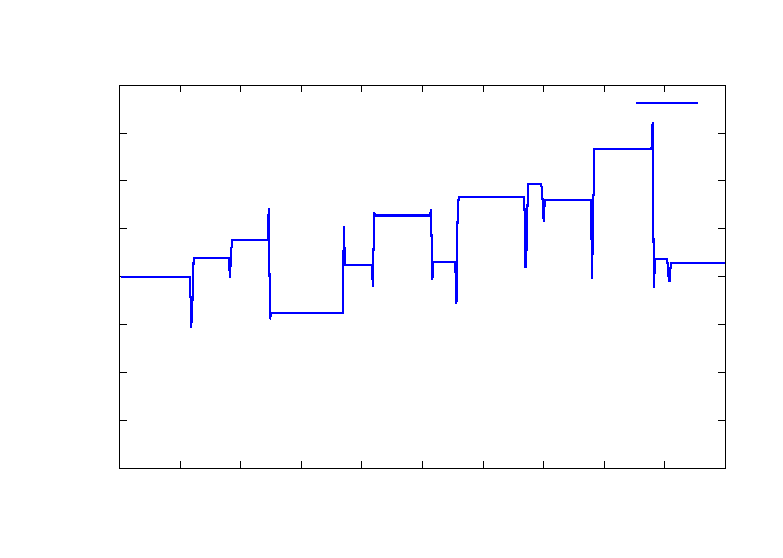
\includegraphics{../Report/figures/E_001_0020}}%
    \gplfronttext
  \end{picture}%
\endgroup
}
			\caption{Energy drift of one particle with $\Delta t=0.02$}
		\end{subfigure}
		\caption{\label{energy-timestep}Energy drift of one particle with different values of time step $dt$, the initial energy is set to 40}
	\end{figure*}
	In figure \ref{energy-timestep} the different energies for the paths in figure \ref{fig:path} is plotted over time. Here we can also see that the energy drift with a time-step of $\Delta t = 0.01$ is not too bad, this is thus a candidate for the highest time-step that gives a stable simulation.
	
	
	\section{Multiple particles}
	
		For all the simulations beyond 1 particle the time step is set to $\Delta t =0.001$, this is because of the stability it provides and the short run time for even very large systems, in tests of time at 40 and particles above 100 the run time does not exceed a few seconds. In the case of two particles the start positions and velocities are chosen, but in larger systems this is done randomly with the velocities such that each particle starts with a kinetic energy of the EPP value. The box size is also increased to $40\times40$. Before we can simulate gases we check that the system handles collisions of particles. The EPP value is set to 30.
		\begin{figure*}[htb]
			\centering
			\begin{subfigure}{.45\textwidth}
				\hspace*{-2cm}\scalebox{0.8}{% GNUPLOT: LaTeX picture with Postscript
\begingroup
  \makeatletter
  \providecommand\color[2][]{%
    \GenericError{(gnuplot) \space\space\space\@spaces}{%
      Package color not loaded in conjunction with
      terminal option `colourtext'%
    }{See the gnuplot documentation for explanation.%
    }{Either use 'blacktext' in gnuplot or load the package
      color.sty in LaTeX.}%
    \renewcommand\color[2][]{}%
  }%
  \providecommand\includegraphics[2][]{%
    \GenericError{(gnuplot) \space\space\space\@spaces}{%
      Package graphicx or graphics not loaded%
    }{See the gnuplot documentation for explanation.%
    }{The gnuplot epslatex terminal needs graphicx.sty or graphics.sty.}%
    \renewcommand\includegraphics[2][]{}%
  }%
  \providecommand\rotatebox[2]{#2}%
  \@ifundefined{ifGPcolor}{%
    \newif\ifGPcolor
    \GPcolortrue
  }{}%
  \@ifundefined{ifGPblacktext}{%
    \newif\ifGPblacktext
    \GPblacktexttrue
  }{}%
  % define a \g@addto@macro without @ in the name:
  \let\gplgaddtomacro\g@addto@macro
  % define empty templates for all commands taking text:
  \gdef\gplbacktext{}%
  \gdef\gplfronttext{}%
  \makeatother
  \ifGPblacktext
    % no textcolor at all
    \def\colorrgb#1{}%
    \def\colorgray#1{}%
  \else
    % gray or color?
    \ifGPcolor
      \def\colorrgb#1{\color[rgb]{#1}}%
      \def\colorgray#1{\color[gray]{#1}}%
      \expandafter\def\csname LTw\endcsname{\color{white}}%
      \expandafter\def\csname LTb\endcsname{\color{black}}%
      \expandafter\def\csname LTa\endcsname{\color{black}}%
      \expandafter\def\csname LT0\endcsname{\color[rgb]{1,0,0}}%
      \expandafter\def\csname LT1\endcsname{\color[rgb]{0,1,0}}%
      \expandafter\def\csname LT2\endcsname{\color[rgb]{0,0,1}}%
      \expandafter\def\csname LT3\endcsname{\color[rgb]{1,0,1}}%
      \expandafter\def\csname LT4\endcsname{\color[rgb]{0,1,1}}%
      \expandafter\def\csname LT5\endcsname{\color[rgb]{1,1,0}}%
      \expandafter\def\csname LT6\endcsname{\color[rgb]{0,0,0}}%
      \expandafter\def\csname LT7\endcsname{\color[rgb]{1,0.3,0}}%
      \expandafter\def\csname LT8\endcsname{\color[rgb]{0.5,0.5,0.5}}%
    \else
      % gray
      \def\colorrgb#1{\color{black}}%
      \def\colorgray#1{\color[gray]{#1}}%
      \expandafter\def\csname LTw\endcsname{\color{white}}%
      \expandafter\def\csname LTb\endcsname{\color{black}}%
      \expandafter\def\csname LTa\endcsname{\color{black}}%
      \expandafter\def\csname LT0\endcsname{\color{black}}%
      \expandafter\def\csname LT1\endcsname{\color{black}}%
      \expandafter\def\csname LT2\endcsname{\color{black}}%
      \expandafter\def\csname LT3\endcsname{\color{black}}%
      \expandafter\def\csname LT4\endcsname{\color{black}}%
      \expandafter\def\csname LT5\endcsname{\color{black}}%
      \expandafter\def\csname LT6\endcsname{\color{black}}%
      \expandafter\def\csname LT7\endcsname{\color{black}}%
      \expandafter\def\csname LT8\endcsname{\color{black}}%
    \fi
  \fi
    \setlength{\unitlength}{0.0500bp}%
    \ifx\gptboxheight\undefined%
      \newlength{\gptboxheight}%
      \newlength{\gptboxwidth}%
      \newsavebox{\gptboxtext}%
    \fi%
    \setlength{\fboxrule}{0.5pt}%
    \setlength{\fboxsep}{1pt}%
\begin{picture}(7200.00,5040.00)%
    \gplgaddtomacro\gplbacktext{%
      \csname LTb\endcsname%%
      \put(1927,704){\makebox(0,0)[r]{\strut{}$-2$}}%
      \put(1927,1229){\makebox(0,0)[r]{\strut{}$0$}}%
      \put(1927,1754){\makebox(0,0)[r]{\strut{}$2$}}%
      \put(1927,2279){\makebox(0,0)[r]{\strut{}$4$}}%
      \put(1927,2804){\makebox(0,0)[r]{\strut{}$6$}}%
      \put(1927,3329){\makebox(0,0)[r]{\strut{}$8$}}%
      \put(1927,3854){\makebox(0,0)[r]{\strut{}$10$}}%
      \put(1927,4379){\makebox(0,0)[r]{\strut{}$12$}}%
      \put(2059,484){\makebox(0,0){\strut{}$-2$}}%
      \put(2584,484){\makebox(0,0){\strut{}$0$}}%
      \put(3109,484){\makebox(0,0){\strut{}$2$}}%
      \put(3634,484){\makebox(0,0){\strut{}$4$}}%
      \put(4159,484){\makebox(0,0){\strut{}$6$}}%
      \put(4684,484){\makebox(0,0){\strut{}$8$}}%
      \put(5209,484){\makebox(0,0){\strut{}$10$}}%
      \put(5734,484){\makebox(0,0){\strut{}$12$}}%
    }%
    \gplgaddtomacro\gplfronttext{%
      \csname LTb\endcsname%%
      \put(1366,2541){\makebox(0,0){\strut{}y}}%
      \put(3896,154){\makebox(0,0){\strut{}x}}%
      \put(3896,4709){\makebox(0,0){\strut{}Trajectory of 2 particles}}%
    }%
    \gplbacktext
    \put(0,0){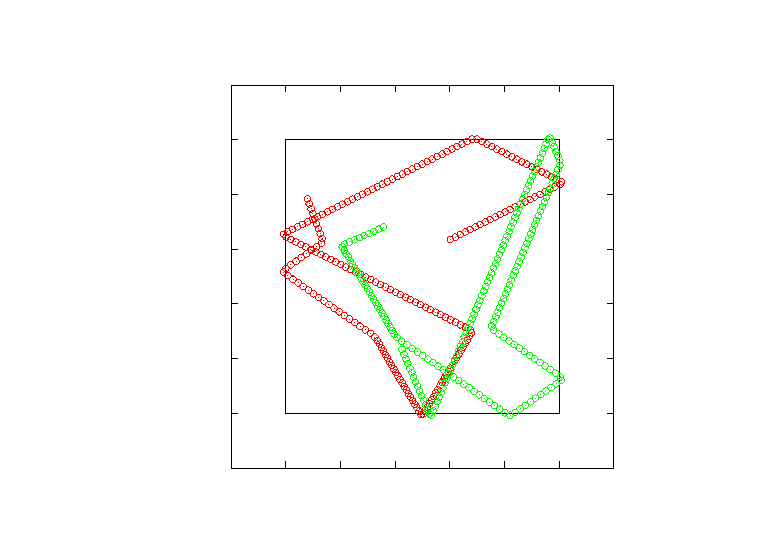
\includegraphics{../Report/figures/P_002_005}}%
    \gplfronttext
  \end{picture}%
\endgroup
}
				\caption{Path of two particles, with collisions}
			\end{subfigure}
			\begin{subfigure}{.45\textwidth}
				\scalebox{0.6}{% GNUPLOT: LaTeX picture with Postscript
\begingroup
  \makeatletter
  \providecommand\color[2][]{%
    \GenericError{(gnuplot) \space\space\space\@spaces}{%
      Package color not loaded in conjunction with
      terminal option `colourtext'%
    }{See the gnuplot documentation for explanation.%
    }{Either use 'blacktext' in gnuplot or load the package
      color.sty in LaTeX.}%
    \renewcommand\color[2][]{}%
  }%
  \providecommand\includegraphics[2][]{%
    \GenericError{(gnuplot) \space\space\space\@spaces}{%
      Package graphicx or graphics not loaded%
    }{See the gnuplot documentation for explanation.%
    }{The gnuplot epslatex terminal needs graphicx.sty or graphics.sty.}%
    \renewcommand\includegraphics[2][]{}%
  }%
  \providecommand\rotatebox[2]{#2}%
  \@ifundefined{ifGPcolor}{%
    \newif\ifGPcolor
    \GPcolortrue
  }{}%
  \@ifundefined{ifGPblacktext}{%
    \newif\ifGPblacktext
    \GPblacktexttrue
  }{}%
  % define a \g@addto@macro without @ in the name:
  \let\gplgaddtomacro\g@addto@macro
  % define empty templates for all commands taking text:
  \gdef\gplbacktext{}%
  \gdef\gplfronttext{}%
  \makeatother
  \ifGPblacktext
    % no textcolor at all
    \def\colorrgb#1{}%
    \def\colorgray#1{}%
  \else
    % gray or color?
    \ifGPcolor
      \def\colorrgb#1{\color[rgb]{#1}}%
      \def\colorgray#1{\color[gray]{#1}}%
      \expandafter\def\csname LTw\endcsname{\color{white}}%
      \expandafter\def\csname LTb\endcsname{\color{black}}%
      \expandafter\def\csname LTa\endcsname{\color{black}}%
      \expandafter\def\csname LT0\endcsname{\color[rgb]{1,0,0}}%
      \expandafter\def\csname LT1\endcsname{\color[rgb]{0,1,0}}%
      \expandafter\def\csname LT2\endcsname{\color[rgb]{0,0,1}}%
      \expandafter\def\csname LT3\endcsname{\color[rgb]{1,0,1}}%
      \expandafter\def\csname LT4\endcsname{\color[rgb]{0,1,1}}%
      \expandafter\def\csname LT5\endcsname{\color[rgb]{1,1,0}}%
      \expandafter\def\csname LT6\endcsname{\color[rgb]{0,0,0}}%
      \expandafter\def\csname LT7\endcsname{\color[rgb]{1,0.3,0}}%
      \expandafter\def\csname LT8\endcsname{\color[rgb]{0.5,0.5,0.5}}%
    \else
      % gray
      \def\colorrgb#1{\color{black}}%
      \def\colorgray#1{\color[gray]{#1}}%
      \expandafter\def\csname LTw\endcsname{\color{white}}%
      \expandafter\def\csname LTb\endcsname{\color{black}}%
      \expandafter\def\csname LTa\endcsname{\color{black}}%
      \expandafter\def\csname LT0\endcsname{\color{black}}%
      \expandafter\def\csname LT1\endcsname{\color{black}}%
      \expandafter\def\csname LT2\endcsname{\color{black}}%
      \expandafter\def\csname LT3\endcsname{\color{black}}%
      \expandafter\def\csname LT4\endcsname{\color{black}}%
      \expandafter\def\csname LT5\endcsname{\color{black}}%
      \expandafter\def\csname LT6\endcsname{\color{black}}%
      \expandafter\def\csname LT7\endcsname{\color{black}}%
      \expandafter\def\csname LT8\endcsname{\color{black}}%
    \fi
  \fi
    \setlength{\unitlength}{0.0500bp}%
    \ifx\gptboxheight\undefined%
      \newlength{\gptboxheight}%
      \newlength{\gptboxwidth}%
      \newsavebox{\gptboxtext}%
    \fi%
    \setlength{\fboxrule}{0.5pt}%
    \setlength{\fboxsep}{1pt}%
\begin{picture}(7200.00,5040.00)%
    \gplgaddtomacro\gplbacktext{%
      \csname LTb\endcsname%%
      \put(682,704){\makebox(0,0)[r]{\strut{}$0$}}%
      \put(682,1163){\makebox(0,0)[r]{\strut{}$5$}}%
      \put(682,1623){\makebox(0,0)[r]{\strut{}$10$}}%
      \put(682,2082){\makebox(0,0)[r]{\strut{}$15$}}%
      \put(682,2542){\makebox(0,0)[r]{\strut{}$20$}}%
      \put(682,3001){\makebox(0,0)[r]{\strut{}$25$}}%
      \put(682,3460){\makebox(0,0)[r]{\strut{}$30$}}%
      \put(682,3920){\makebox(0,0)[r]{\strut{}$35$}}%
      \put(682,4379){\makebox(0,0)[r]{\strut{}$40$}}%
      \put(814,484){\makebox(0,0){\strut{}$0$}}%
      \put(1413,484){\makebox(0,0){\strut{}$0.5$}}%
      \put(2012,484){\makebox(0,0){\strut{}$1$}}%
      \put(2611,484){\makebox(0,0){\strut{}$1.5$}}%
      \put(3210,484){\makebox(0,0){\strut{}$2$}}%
      \put(3809,484){\makebox(0,0){\strut{}$2.5$}}%
      \put(4407,484){\makebox(0,0){\strut{}$3$}}%
      \put(5006,484){\makebox(0,0){\strut{}$3.5$}}%
      \put(5605,484){\makebox(0,0){\strut{}$4$}}%
      \put(6204,484){\makebox(0,0){\strut{}$4.5$}}%
      \put(6803,484){\makebox(0,0){\strut{}$5$}}%
    }%
    \gplgaddtomacro\gplfronttext{%
      \csname LTb\endcsname%%
      \put(209,2541){\rotatebox{-270}{\makebox(0,0){\strut{}E}}}%
      \put(3808,154){\makebox(0,0){\strut{}T}}%
      \put(3808,4709){\makebox(0,0){\strut{}Total energy per particle of 2 particles}}%
      \csname LTb\endcsname%%
      \put(5816,4206){\makebox(0,0)[r]{\strut{}Energy}}%
    }%
    \gplbacktext
    \put(0,0){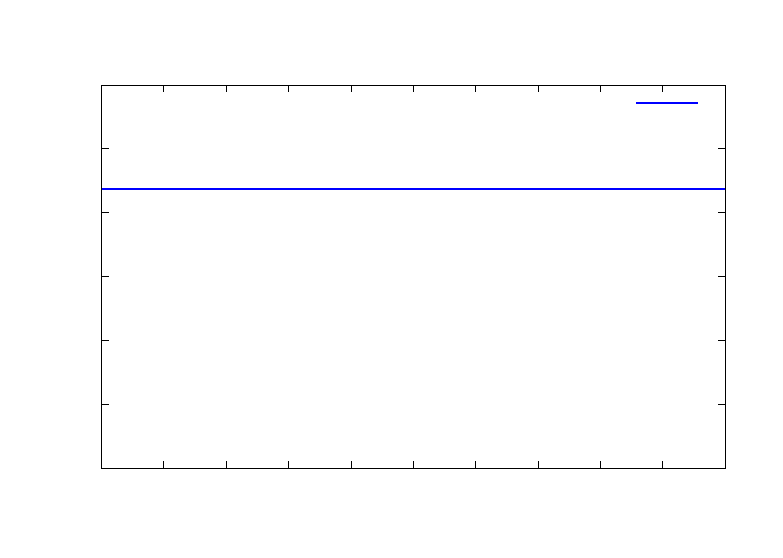
\includegraphics{../Report/figures/E_002_005}}%
    \gplfronttext
  \end{picture}%
\endgroup
}
				\caption{Total energy per particle of the two particles as the collisions happen}
			\end{subfigure}
			\caption{\label{two-collide}Two particles over a short time scale}
		\end{figure*}
		
		\begin{figure*}[htb]
			\centering
			\begin{subfigure}{.45\textwidth}
				\hspace*{-2cm}\scalebox{0.8}{% GNUPLOT: LaTeX picture with Postscript
\begingroup
  % Encoding inside the plot.  In the header of your document, this encoding
  % should to defined, e.g., by using
  % \usepackage[cp1252,<other encodings>]{inputenc}
  \inputencoding{cp1252}%
  \makeatletter
  \providecommand\color[2][]{%
    \GenericError{(gnuplot) \space\space\space\@spaces}{%
      Package color not loaded in conjunction with
      terminal option `colourtext'%
    }{See the gnuplot documentation for explanation.%
    }{Either use 'blacktext' in gnuplot or load the package
      color.sty in LaTeX.}%
    \renewcommand\color[2][]{}%
  }%
  \providecommand\includegraphics[2][]{%
    \GenericError{(gnuplot) \space\space\space\@spaces}{%
      Package graphicx or graphics not loaded%
    }{See the gnuplot documentation for explanation.%
    }{The gnuplot epslatex terminal needs graphicx.sty or graphics.sty.}%
    \renewcommand\includegraphics[2][]{}%
  }%
  \providecommand\rotatebox[2]{#2}%
  \@ifundefined{ifGPcolor}{%
    \newif\ifGPcolor
    \GPcolortrue
  }{}%
  \@ifundefined{ifGPblacktext}{%
    \newif\ifGPblacktext
    \GPblacktexttrue
  }{}%
  % define a \g@addto@macro without @ in the name:
  \let\gplgaddtomacro\g@addto@macro
  % define empty templates for all commands taking text:
  \gdef\gplbacktext{}%
  \gdef\gplfronttext{}%
  \makeatother
  \ifGPblacktext
    % no textcolor at all
    \def\colorrgb#1{}%
    \def\colorgray#1{}%
  \else
    % gray or color?
    \ifGPcolor
      \def\colorrgb#1{\color[rgb]{#1}}%
      \def\colorgray#1{\color[gray]{#1}}%
      \expandafter\def\csname LTw\endcsname{\color{white}}%
      \expandafter\def\csname LTb\endcsname{\color{black}}%
      \expandafter\def\csname LTa\endcsname{\color{black}}%
      \expandafter\def\csname LT0\endcsname{\color[rgb]{1,0,0}}%
      \expandafter\def\csname LT1\endcsname{\color[rgb]{0,1,0}}%
      \expandafter\def\csname LT2\endcsname{\color[rgb]{0,0,1}}%
      \expandafter\def\csname LT3\endcsname{\color[rgb]{1,0,1}}%
      \expandafter\def\csname LT4\endcsname{\color[rgb]{0,1,1}}%
      \expandafter\def\csname LT5\endcsname{\color[rgb]{1,1,0}}%
      \expandafter\def\csname LT6\endcsname{\color[rgb]{0,0,0}}%
      \expandafter\def\csname LT7\endcsname{\color[rgb]{1,0.3,0}}%
      \expandafter\def\csname LT8\endcsname{\color[rgb]{0.5,0.5,0.5}}%
    \else
      % gray
      \def\colorrgb#1{\color{black}}%
      \def\colorgray#1{\color[gray]{#1}}%
      \expandafter\def\csname LTw\endcsname{\color{white}}%
      \expandafter\def\csname LTb\endcsname{\color{black}}%
      \expandafter\def\csname LTa\endcsname{\color{black}}%
      \expandafter\def\csname LT0\endcsname{\color{black}}%
      \expandafter\def\csname LT1\endcsname{\color{black}}%
      \expandafter\def\csname LT2\endcsname{\color{black}}%
      \expandafter\def\csname LT3\endcsname{\color{black}}%
      \expandafter\def\csname LT4\endcsname{\color{black}}%
      \expandafter\def\csname LT5\endcsname{\color{black}}%
      \expandafter\def\csname LT6\endcsname{\color{black}}%
      \expandafter\def\csname LT7\endcsname{\color{black}}%
      \expandafter\def\csname LT8\endcsname{\color{black}}%
    \fi
  \fi
    \setlength{\unitlength}{0.0500bp}%
    \ifx\gptboxheight\undefined%
      \newlength{\gptboxheight}%
      \newlength{\gptboxwidth}%
      \newsavebox{\gptboxtext}%
    \fi%
    \setlength{\fboxrule}{0.5pt}%
    \setlength{\fboxsep}{1pt}%
\begin{picture}(7200.00,5040.00)%
    \gplgaddtomacro\gplbacktext{%
      \csname LTb\endcsname%%
      \put(1927,704){\makebox(0,0)[r]{\strut{}$-2$}}%
      \put(1927,1229){\makebox(0,0)[r]{\strut{}$0$}}%
      \put(1927,1754){\makebox(0,0)[r]{\strut{}$2$}}%
      \put(1927,2279){\makebox(0,0)[r]{\strut{}$4$}}%
      \put(1927,2804){\makebox(0,0)[r]{\strut{}$6$}}%
      \put(1927,3329){\makebox(0,0)[r]{\strut{}$8$}}%
      \put(1927,3854){\makebox(0,0)[r]{\strut{}$10$}}%
      \put(1927,4379){\makebox(0,0)[r]{\strut{}$12$}}%
      \put(2059,484){\makebox(0,0){\strut{}$-2$}}%
      \put(2584,484){\makebox(0,0){\strut{}$0$}}%
      \put(3109,484){\makebox(0,0){\strut{}$2$}}%
      \put(3634,484){\makebox(0,0){\strut{}$4$}}%
      \put(4159,484){\makebox(0,0){\strut{}$6$}}%
      \put(4684,484){\makebox(0,0){\strut{}$8$}}%
      \put(5209,484){\makebox(0,0){\strut{}$10$}}%
      \put(5734,484){\makebox(0,0){\strut{}$12$}}%
    }%
    \gplgaddtomacro\gplfronttext{%
      \csname LTb\endcsname%%
      \put(1465,2541){\makebox(0,0){\strut{}y}}%
      \put(3896,154){\makebox(0,0){\strut{}x}}%
      \put(3896,4709){\makebox(0,0){\strut{}Trajectory of 3 particles}}%
    }%
    \gplbacktext
    \put(0,0){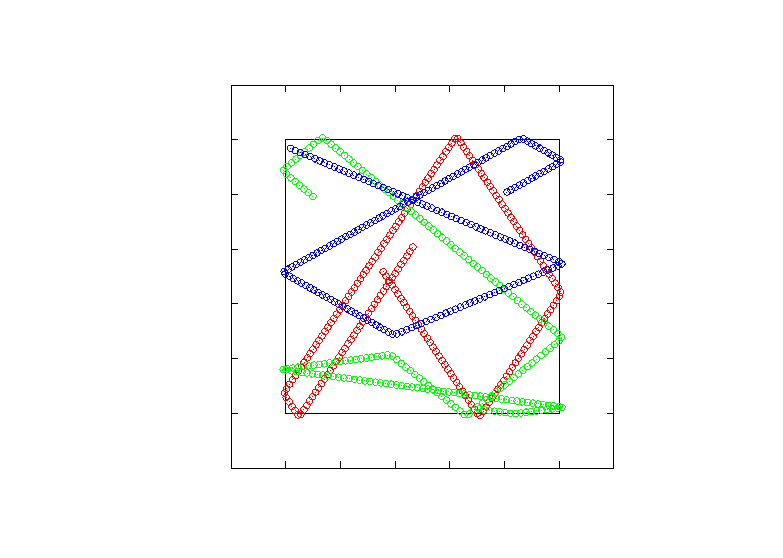
\includegraphics{../Report/figures/P_003_005}}%
    \gplfronttext
  \end{picture}%
\endgroup
}
				\caption{Path of three particles, with collisions}
			\end{subfigure}
			\begin{subfigure}{.45\textwidth}
				\scalebox{0.6}{% GNUPLOT: LaTeX picture with Postscript
\begingroup
  \makeatletter
  \providecommand\color[2][]{%
    \GenericError{(gnuplot) \space\space\space\@spaces}{%
      Package color not loaded in conjunction with
      terminal option `colourtext'%
    }{See the gnuplot documentation for explanation.%
    }{Either use 'blacktext' in gnuplot or load the package
      color.sty in LaTeX.}%
    \renewcommand\color[2][]{}%
  }%
  \providecommand\includegraphics[2][]{%
    \GenericError{(gnuplot) \space\space\space\@spaces}{%
      Package graphicx or graphics not loaded%
    }{See the gnuplot documentation for explanation.%
    }{The gnuplot epslatex terminal needs graphicx.sty or graphics.sty.}%
    \renewcommand\includegraphics[2][]{}%
  }%
  \providecommand\rotatebox[2]{#2}%
  \@ifundefined{ifGPcolor}{%
    \newif\ifGPcolor
    \GPcolortrue
  }{}%
  \@ifundefined{ifGPblacktext}{%
    \newif\ifGPblacktext
    \GPblacktexttrue
  }{}%
  % define a \g@addto@macro without @ in the name:
  \let\gplgaddtomacro\g@addto@macro
  % define empty templates for all commands taking text:
  \gdef\gplbacktext{}%
  \gdef\gplfronttext{}%
  \makeatother
  \ifGPblacktext
    % no textcolor at all
    \def\colorrgb#1{}%
    \def\colorgray#1{}%
  \else
    % gray or color?
    \ifGPcolor
      \def\colorrgb#1{\color[rgb]{#1}}%
      \def\colorgray#1{\color[gray]{#1}}%
      \expandafter\def\csname LTw\endcsname{\color{white}}%
      \expandafter\def\csname LTb\endcsname{\color{black}}%
      \expandafter\def\csname LTa\endcsname{\color{black}}%
      \expandafter\def\csname LT0\endcsname{\color[rgb]{1,0,0}}%
      \expandafter\def\csname LT1\endcsname{\color[rgb]{0,1,0}}%
      \expandafter\def\csname LT2\endcsname{\color[rgb]{0,0,1}}%
      \expandafter\def\csname LT3\endcsname{\color[rgb]{1,0,1}}%
      \expandafter\def\csname LT4\endcsname{\color[rgb]{0,1,1}}%
      \expandafter\def\csname LT5\endcsname{\color[rgb]{1,1,0}}%
      \expandafter\def\csname LT6\endcsname{\color[rgb]{0,0,0}}%
      \expandafter\def\csname LT7\endcsname{\color[rgb]{1,0.3,0}}%
      \expandafter\def\csname LT8\endcsname{\color[rgb]{0.5,0.5,0.5}}%
    \else
      % gray
      \def\colorrgb#1{\color{black}}%
      \def\colorgray#1{\color[gray]{#1}}%
      \expandafter\def\csname LTw\endcsname{\color{white}}%
      \expandafter\def\csname LTb\endcsname{\color{black}}%
      \expandafter\def\csname LTa\endcsname{\color{black}}%
      \expandafter\def\csname LT0\endcsname{\color{black}}%
      \expandafter\def\csname LT1\endcsname{\color{black}}%
      \expandafter\def\csname LT2\endcsname{\color{black}}%
      \expandafter\def\csname LT3\endcsname{\color{black}}%
      \expandafter\def\csname LT4\endcsname{\color{black}}%
      \expandafter\def\csname LT5\endcsname{\color{black}}%
      \expandafter\def\csname LT6\endcsname{\color{black}}%
      \expandafter\def\csname LT7\endcsname{\color{black}}%
      \expandafter\def\csname LT8\endcsname{\color{black}}%
    \fi
  \fi
    \setlength{\unitlength}{0.0500bp}%
    \ifx\gptboxheight\undefined%
      \newlength{\gptboxheight}%
      \newlength{\gptboxwidth}%
      \newsavebox{\gptboxtext}%
    \fi%
    \setlength{\fboxrule}{0.5pt}%
    \setlength{\fboxsep}{1pt}%
\begin{picture}(7200.00,5040.00)%
    \gplgaddtomacro\gplbacktext{%
      \csname LTb\endcsname%%
      \put(682,704){\makebox(0,0)[r]{\strut{}$0$}}%
      \put(682,1163){\makebox(0,0)[r]{\strut{}$5$}}%
      \put(682,1623){\makebox(0,0)[r]{\strut{}$10$}}%
      \put(682,2082){\makebox(0,0)[r]{\strut{}$15$}}%
      \put(682,2542){\makebox(0,0)[r]{\strut{}$20$}}%
      \put(682,3001){\makebox(0,0)[r]{\strut{}$25$}}%
      \put(682,3460){\makebox(0,0)[r]{\strut{}$30$}}%
      \put(682,3920){\makebox(0,0)[r]{\strut{}$35$}}%
      \put(682,4379){\makebox(0,0)[r]{\strut{}$40$}}%
      \put(814,484){\makebox(0,0){\strut{}$0$}}%
      \put(1413,484){\makebox(0,0){\strut{}$0.5$}}%
      \put(2012,484){\makebox(0,0){\strut{}$1$}}%
      \put(2611,484){\makebox(0,0){\strut{}$1.5$}}%
      \put(3210,484){\makebox(0,0){\strut{}$2$}}%
      \put(3809,484){\makebox(0,0){\strut{}$2.5$}}%
      \put(4407,484){\makebox(0,0){\strut{}$3$}}%
      \put(5006,484){\makebox(0,0){\strut{}$3.5$}}%
      \put(5605,484){\makebox(0,0){\strut{}$4$}}%
      \put(6204,484){\makebox(0,0){\strut{}$4.5$}}%
      \put(6803,484){\makebox(0,0){\strut{}$5$}}%
    }%
    \gplgaddtomacro\gplfronttext{%
      \csname LTb\endcsname%%
      \put(209,2541){\rotatebox{-270}{\makebox(0,0){\strut{}E}}}%
      \put(3808,154){\makebox(0,0){\strut{}T}}%
      \put(3808,4709){\makebox(0,0){\strut{}Total energy per particle of 3 particles}}%
      \csname LTb\endcsname%%
      \put(5816,4206){\makebox(0,0)[r]{\strut{}Energy}}%
    }%
    \gplbacktext
    \put(0,0){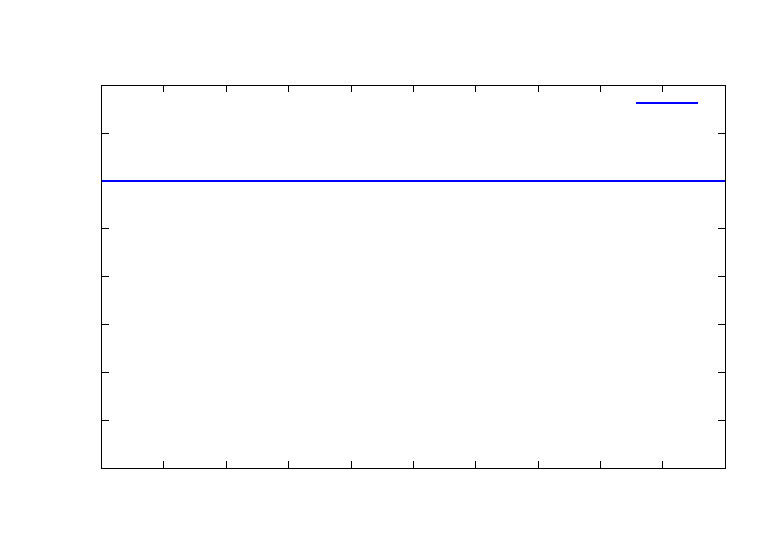
\includegraphics{../Report/figures/E_003_005}}%
    \gplfronttext
  \end{picture}%
\endgroup
}
				\caption{Total energy per particle of the three particles as the collisions happen}
			\end{subfigure}
			\caption{\label{three-collide}Three particles over a short time scale}
		\end{figure*}
		
		\begin{figure*}[htb]
			\centering
			\begin{subfigure}{.45\textwidth}
				\hspace*{-2cm}\scalebox{0.8}{% GNUPLOT: LaTeX picture with Postscript
\begingroup
  % Encoding inside the plot.  In the header of your document, this encoding
  % should to defined, e.g., by using
  % \usepackage[cp1252,<other encodings>]{inputenc}
  \inputencoding{cp1252}%
  \makeatletter
  \providecommand\color[2][]{%
    \GenericError{(gnuplot) \space\space\space\@spaces}{%
      Package color not loaded in conjunction with
      terminal option `colourtext'%
    }{See the gnuplot documentation for explanation.%
    }{Either use 'blacktext' in gnuplot or load the package
      color.sty in LaTeX.}%
    \renewcommand\color[2][]{}%
  }%
  \providecommand\includegraphics[2][]{%
    \GenericError{(gnuplot) \space\space\space\@spaces}{%
      Package graphicx or graphics not loaded%
    }{See the gnuplot documentation for explanation.%
    }{The gnuplot epslatex terminal needs graphicx.sty or graphics.sty.}%
    \renewcommand\includegraphics[2][]{}%
  }%
  \providecommand\rotatebox[2]{#2}%
  \@ifundefined{ifGPcolor}{%
    \newif\ifGPcolor
    \GPcolortrue
  }{}%
  \@ifundefined{ifGPblacktext}{%
    \newif\ifGPblacktext
    \GPblacktexttrue
  }{}%
  % define a \g@addto@macro without @ in the name:
  \let\gplgaddtomacro\g@addto@macro
  % define empty templates for all commands taking text:
  \gdef\gplbacktext{}%
  \gdef\gplfronttext{}%
  \makeatother
  \ifGPblacktext
    % no textcolor at all
    \def\colorrgb#1{}%
    \def\colorgray#1{}%
  \else
    % gray or color?
    \ifGPcolor
      \def\colorrgb#1{\color[rgb]{#1}}%
      \def\colorgray#1{\color[gray]{#1}}%
      \expandafter\def\csname LTw\endcsname{\color{white}}%
      \expandafter\def\csname LTb\endcsname{\color{black}}%
      \expandafter\def\csname LTa\endcsname{\color{black}}%
      \expandafter\def\csname LT0\endcsname{\color[rgb]{1,0,0}}%
      \expandafter\def\csname LT1\endcsname{\color[rgb]{0,1,0}}%
      \expandafter\def\csname LT2\endcsname{\color[rgb]{0,0,1}}%
      \expandafter\def\csname LT3\endcsname{\color[rgb]{1,0,1}}%
      \expandafter\def\csname LT4\endcsname{\color[rgb]{0,1,1}}%
      \expandafter\def\csname LT5\endcsname{\color[rgb]{1,1,0}}%
      \expandafter\def\csname LT6\endcsname{\color[rgb]{0,0,0}}%
      \expandafter\def\csname LT7\endcsname{\color[rgb]{1,0.3,0}}%
      \expandafter\def\csname LT8\endcsname{\color[rgb]{0.5,0.5,0.5}}%
    \else
      % gray
      \def\colorrgb#1{\color{black}}%
      \def\colorgray#1{\color[gray]{#1}}%
      \expandafter\def\csname LTw\endcsname{\color{white}}%
      \expandafter\def\csname LTb\endcsname{\color{black}}%
      \expandafter\def\csname LTa\endcsname{\color{black}}%
      \expandafter\def\csname LT0\endcsname{\color{black}}%
      \expandafter\def\csname LT1\endcsname{\color{black}}%
      \expandafter\def\csname LT2\endcsname{\color{black}}%
      \expandafter\def\csname LT3\endcsname{\color{black}}%
      \expandafter\def\csname LT4\endcsname{\color{black}}%
      \expandafter\def\csname LT5\endcsname{\color{black}}%
      \expandafter\def\csname LT6\endcsname{\color{black}}%
      \expandafter\def\csname LT7\endcsname{\color{black}}%
      \expandafter\def\csname LT8\endcsname{\color{black}}%
    \fi
  \fi
    \setlength{\unitlength}{0.0500bp}%
    \ifx\gptboxheight\undefined%
      \newlength{\gptboxheight}%
      \newlength{\gptboxwidth}%
      \newsavebox{\gptboxtext}%
    \fi%
    \setlength{\fboxrule}{0.5pt}%
    \setlength{\fboxsep}{1pt}%
\begin{picture}(7200.00,5040.00)%
    \gplgaddtomacro\gplbacktext{%
      \csname LTb\endcsname%%
      \put(1927,704){\makebox(0,0)[r]{\strut{}$-2$}}%
      \put(1927,1229){\makebox(0,0)[r]{\strut{}$0$}}%
      \put(1927,1754){\makebox(0,0)[r]{\strut{}$2$}}%
      \put(1927,2279){\makebox(0,0)[r]{\strut{}$4$}}%
      \put(1927,2804){\makebox(0,0)[r]{\strut{}$6$}}%
      \put(1927,3329){\makebox(0,0)[r]{\strut{}$8$}}%
      \put(1927,3854){\makebox(0,0)[r]{\strut{}$10$}}%
      \put(1927,4379){\makebox(0,0)[r]{\strut{}$12$}}%
      \put(2059,484){\makebox(0,0){\strut{}$-2$}}%
      \put(2584,484){\makebox(0,0){\strut{}$0$}}%
      \put(3109,484){\makebox(0,0){\strut{}$2$}}%
      \put(3634,484){\makebox(0,0){\strut{}$4$}}%
      \put(4159,484){\makebox(0,0){\strut{}$6$}}%
      \put(4684,484){\makebox(0,0){\strut{}$8$}}%
      \put(5209,484){\makebox(0,0){\strut{}$10$}}%
      \put(5734,484){\makebox(0,0){\strut{}$12$}}%
    }%
    \gplgaddtomacro\gplfronttext{%
      \csname LTb\endcsname%%
      \put(1465,2541){\makebox(0,0){\strut{}y}}%
      \put(3896,154){\makebox(0,0){\strut{}x}}%
      \put(3896,4709){\makebox(0,0){\strut{}Trajectory of 4 particles}}%
    }%
    \gplbacktext
    \put(0,0){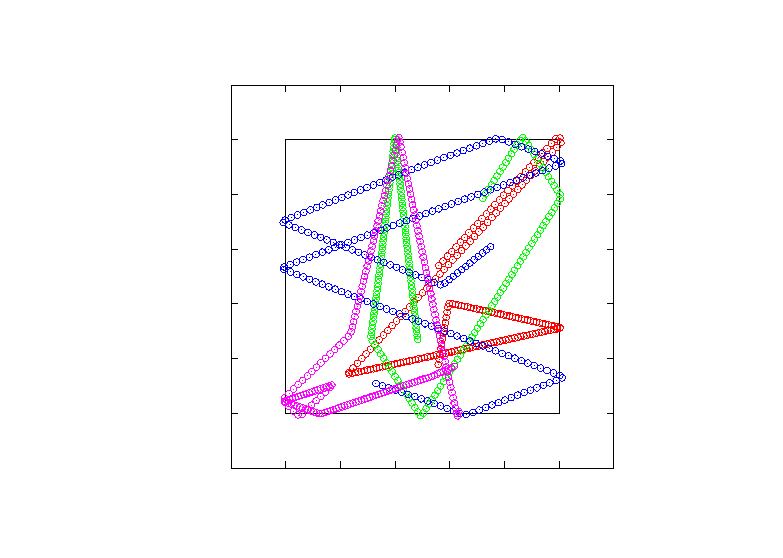
\includegraphics{../Report/figures/P_004_005}}%
    \gplfronttext
  \end{picture}%
\endgroup
}
				\caption{Path of four particles, with collisions}
			\end{subfigure}
			\begin{subfigure}{.45\textwidth}
				\scalebox{0.6}{% GNUPLOT: LaTeX picture with Postscript
\begingroup
  \makeatletter
  \providecommand\color[2][]{%
    \GenericError{(gnuplot) \space\space\space\@spaces}{%
      Package color not loaded in conjunction with
      terminal option `colourtext'%
    }{See the gnuplot documentation for explanation.%
    }{Either use 'blacktext' in gnuplot or load the package
      color.sty in LaTeX.}%
    \renewcommand\color[2][]{}%
  }%
  \providecommand\includegraphics[2][]{%
    \GenericError{(gnuplot) \space\space\space\@spaces}{%
      Package graphicx or graphics not loaded%
    }{See the gnuplot documentation for explanation.%
    }{The gnuplot epslatex terminal needs graphicx.sty or graphics.sty.}%
    \renewcommand\includegraphics[2][]{}%
  }%
  \providecommand\rotatebox[2]{#2}%
  \@ifundefined{ifGPcolor}{%
    \newif\ifGPcolor
    \GPcolortrue
  }{}%
  \@ifundefined{ifGPblacktext}{%
    \newif\ifGPblacktext
    \GPblacktexttrue
  }{}%
  % define a \g@addto@macro without @ in the name:
  \let\gplgaddtomacro\g@addto@macro
  % define empty templates for all commands taking text:
  \gdef\gplbacktext{}%
  \gdef\gplfronttext{}%
  \makeatother
  \ifGPblacktext
    % no textcolor at all
    \def\colorrgb#1{}%
    \def\colorgray#1{}%
  \else
    % gray or color?
    \ifGPcolor
      \def\colorrgb#1{\color[rgb]{#1}}%
      \def\colorgray#1{\color[gray]{#1}}%
      \expandafter\def\csname LTw\endcsname{\color{white}}%
      \expandafter\def\csname LTb\endcsname{\color{black}}%
      \expandafter\def\csname LTa\endcsname{\color{black}}%
      \expandafter\def\csname LT0\endcsname{\color[rgb]{1,0,0}}%
      \expandafter\def\csname LT1\endcsname{\color[rgb]{0,1,0}}%
      \expandafter\def\csname LT2\endcsname{\color[rgb]{0,0,1}}%
      \expandafter\def\csname LT3\endcsname{\color[rgb]{1,0,1}}%
      \expandafter\def\csname LT4\endcsname{\color[rgb]{0,1,1}}%
      \expandafter\def\csname LT5\endcsname{\color[rgb]{1,1,0}}%
      \expandafter\def\csname LT6\endcsname{\color[rgb]{0,0,0}}%
      \expandafter\def\csname LT7\endcsname{\color[rgb]{1,0.3,0}}%
      \expandafter\def\csname LT8\endcsname{\color[rgb]{0.5,0.5,0.5}}%
    \else
      % gray
      \def\colorrgb#1{\color{black}}%
      \def\colorgray#1{\color[gray]{#1}}%
      \expandafter\def\csname LTw\endcsname{\color{white}}%
      \expandafter\def\csname LTb\endcsname{\color{black}}%
      \expandafter\def\csname LTa\endcsname{\color{black}}%
      \expandafter\def\csname LT0\endcsname{\color{black}}%
      \expandafter\def\csname LT1\endcsname{\color{black}}%
      \expandafter\def\csname LT2\endcsname{\color{black}}%
      \expandafter\def\csname LT3\endcsname{\color{black}}%
      \expandafter\def\csname LT4\endcsname{\color{black}}%
      \expandafter\def\csname LT5\endcsname{\color{black}}%
      \expandafter\def\csname LT6\endcsname{\color{black}}%
      \expandafter\def\csname LT7\endcsname{\color{black}}%
      \expandafter\def\csname LT8\endcsname{\color{black}}%
    \fi
  \fi
    \setlength{\unitlength}{0.0500bp}%
    \ifx\gptboxheight\undefined%
      \newlength{\gptboxheight}%
      \newlength{\gptboxwidth}%
      \newsavebox{\gptboxtext}%
    \fi%
    \setlength{\fboxrule}{0.5pt}%
    \setlength{\fboxsep}{1pt}%
\begin{picture}(7200.00,5040.00)%
    \gplgaddtomacro\gplbacktext{%
      \csname LTb\endcsname%%
      \put(682,704){\makebox(0,0)[r]{\strut{}$0$}}%
      \put(682,1163){\makebox(0,0)[r]{\strut{}$5$}}%
      \put(682,1623){\makebox(0,0)[r]{\strut{}$10$}}%
      \put(682,2082){\makebox(0,0)[r]{\strut{}$15$}}%
      \put(682,2542){\makebox(0,0)[r]{\strut{}$20$}}%
      \put(682,3001){\makebox(0,0)[r]{\strut{}$25$}}%
      \put(682,3460){\makebox(0,0)[r]{\strut{}$30$}}%
      \put(682,3920){\makebox(0,0)[r]{\strut{}$35$}}%
      \put(682,4379){\makebox(0,0)[r]{\strut{}$40$}}%
      \put(814,484){\makebox(0,0){\strut{}$0$}}%
      \put(1413,484){\makebox(0,0){\strut{}$0.5$}}%
      \put(2012,484){\makebox(0,0){\strut{}$1$}}%
      \put(2611,484){\makebox(0,0){\strut{}$1.5$}}%
      \put(3210,484){\makebox(0,0){\strut{}$2$}}%
      \put(3809,484){\makebox(0,0){\strut{}$2.5$}}%
      \put(4407,484){\makebox(0,0){\strut{}$3$}}%
      \put(5006,484){\makebox(0,0){\strut{}$3.5$}}%
      \put(5605,484){\makebox(0,0){\strut{}$4$}}%
      \put(6204,484){\makebox(0,0){\strut{}$4.5$}}%
      \put(6803,484){\makebox(0,0){\strut{}$5$}}%
    }%
    \gplgaddtomacro\gplfronttext{%
      \csname LTb\endcsname%%
      \put(209,2541){\rotatebox{-270}{\makebox(0,0){\strut{}E}}}%
      \put(3808,154){\makebox(0,0){\strut{}T}}%
      \put(3808,4709){\makebox(0,0){\strut{}Total energy per particle of 4 particles}}%
      \csname LTb\endcsname%%
      \put(5816,4206){\makebox(0,0)[r]{\strut{}Energy}}%
    }%
    \gplbacktext
    \put(0,0){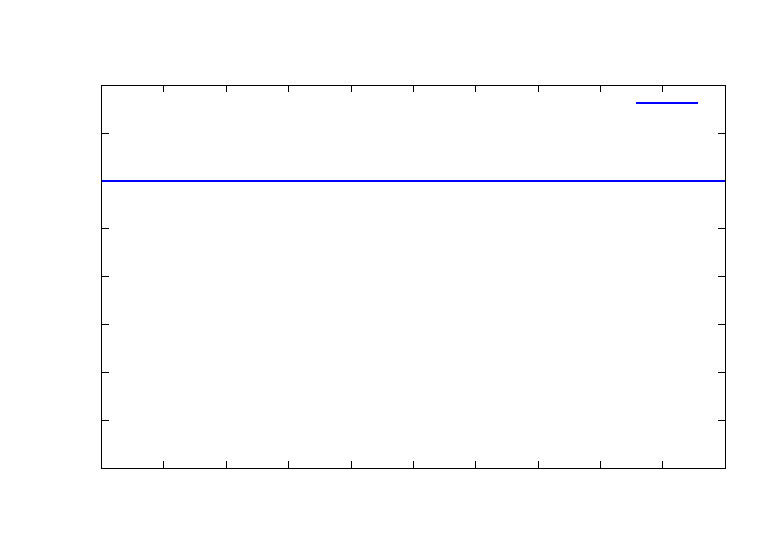
\includegraphics{../Report/figures/E_004_005}}%
    \gplfronttext
  \end{picture}%
\endgroup
}
				\caption{Total energy per particle of the four particles as the collisions happen}
			\end{subfigure}
			\caption{\label{four-collide}Four particles over a short time scale}
		\end{figure*}
		
		\begin{figure*}[htb]
			\centering
			\begin{subfigure}{.45\textwidth}
				\hspace*{-2cm}\scalebox{0.8}{% GNUPLOT: LaTeX picture with Postscript
\begingroup
  \makeatletter
  \providecommand\color[2][]{%
    \GenericError{(gnuplot) \space\space\space\@spaces}{%
      Package color not loaded in conjunction with
      terminal option `colourtext'%
    }{See the gnuplot documentation for explanation.%
    }{Either use 'blacktext' in gnuplot or load the package
      color.sty in LaTeX.}%
    \renewcommand\color[2][]{}%
  }%
  \providecommand\includegraphics[2][]{%
    \GenericError{(gnuplot) \space\space\space\@spaces}{%
      Package graphicx or graphics not loaded%
    }{See the gnuplot documentation for explanation.%
    }{The gnuplot epslatex terminal needs graphicx.sty or graphics.sty.}%
    \renewcommand\includegraphics[2][]{}%
  }%
  \providecommand\rotatebox[2]{#2}%
  \@ifundefined{ifGPcolor}{%
    \newif\ifGPcolor
    \GPcolortrue
  }{}%
  \@ifundefined{ifGPblacktext}{%
    \newif\ifGPblacktext
    \GPblacktexttrue
  }{}%
  % define a \g@addto@macro without @ in the name:
  \let\gplgaddtomacro\g@addto@macro
  % define empty templates for all commands taking text:
  \gdef\gplbacktext{}%
  \gdef\gplfronttext{}%
  \makeatother
  \ifGPblacktext
    % no textcolor at all
    \def\colorrgb#1{}%
    \def\colorgray#1{}%
  \else
    % gray or color?
    \ifGPcolor
      \def\colorrgb#1{\color[rgb]{#1}}%
      \def\colorgray#1{\color[gray]{#1}}%
      \expandafter\def\csname LTw\endcsname{\color{white}}%
      \expandafter\def\csname LTb\endcsname{\color{black}}%
      \expandafter\def\csname LTa\endcsname{\color{black}}%
      \expandafter\def\csname LT0\endcsname{\color[rgb]{1,0,0}}%
      \expandafter\def\csname LT1\endcsname{\color[rgb]{0,1,0}}%
      \expandafter\def\csname LT2\endcsname{\color[rgb]{0,0,1}}%
      \expandafter\def\csname LT3\endcsname{\color[rgb]{1,0,1}}%
      \expandafter\def\csname LT4\endcsname{\color[rgb]{0,1,1}}%
      \expandafter\def\csname LT5\endcsname{\color[rgb]{1,1,0}}%
      \expandafter\def\csname LT6\endcsname{\color[rgb]{0,0,0}}%
      \expandafter\def\csname LT7\endcsname{\color[rgb]{1,0.3,0}}%
      \expandafter\def\csname LT8\endcsname{\color[rgb]{0.5,0.5,0.5}}%
    \else
      % gray
      \def\colorrgb#1{\color{black}}%
      \def\colorgray#1{\color[gray]{#1}}%
      \expandafter\def\csname LTw\endcsname{\color{white}}%
      \expandafter\def\csname LTb\endcsname{\color{black}}%
      \expandafter\def\csname LTa\endcsname{\color{black}}%
      \expandafter\def\csname LT0\endcsname{\color{black}}%
      \expandafter\def\csname LT1\endcsname{\color{black}}%
      \expandafter\def\csname LT2\endcsname{\color{black}}%
      \expandafter\def\csname LT3\endcsname{\color{black}}%
      \expandafter\def\csname LT4\endcsname{\color{black}}%
      \expandafter\def\csname LT5\endcsname{\color{black}}%
      \expandafter\def\csname LT6\endcsname{\color{black}}%
      \expandafter\def\csname LT7\endcsname{\color{black}}%
      \expandafter\def\csname LT8\endcsname{\color{black}}%
    \fi
  \fi
    \setlength{\unitlength}{0.0500bp}%
    \ifx\gptboxheight\undefined%
      \newlength{\gptboxheight}%
      \newlength{\gptboxwidth}%
      \newsavebox{\gptboxtext}%
    \fi%
    \setlength{\fboxrule}{0.5pt}%
    \setlength{\fboxsep}{1pt}%
\begin{picture}(7200.00,5040.00)%
    \gplgaddtomacro\gplbacktext{%
      \csname LTb\endcsname%%
      \put(1927,704){\makebox(0,0)[r]{\strut{}$-2$}}%
      \put(1927,1229){\makebox(0,0)[r]{\strut{}$0$}}%
      \put(1927,1754){\makebox(0,0)[r]{\strut{}$2$}}%
      \put(1927,2279){\makebox(0,0)[r]{\strut{}$4$}}%
      \put(1927,2804){\makebox(0,0)[r]{\strut{}$6$}}%
      \put(1927,3329){\makebox(0,0)[r]{\strut{}$8$}}%
      \put(1927,3854){\makebox(0,0)[r]{\strut{}$10$}}%
      \put(1927,4379){\makebox(0,0)[r]{\strut{}$12$}}%
      \put(2059,484){\makebox(0,0){\strut{}$-2$}}%
      \put(2584,484){\makebox(0,0){\strut{}$0$}}%
      \put(3109,484){\makebox(0,0){\strut{}$2$}}%
      \put(3634,484){\makebox(0,0){\strut{}$4$}}%
      \put(4159,484){\makebox(0,0){\strut{}$6$}}%
      \put(4684,484){\makebox(0,0){\strut{}$8$}}%
      \put(5209,484){\makebox(0,0){\strut{}$10$}}%
      \put(5734,484){\makebox(0,0){\strut{}$12$}}%
    }%
    \gplgaddtomacro\gplfronttext{%
      \csname LTb\endcsname%%
      \put(1366,2541){\makebox(0,0){\strut{}y}}%
      \put(3896,154){\makebox(0,0){\strut{}x}}%
      \put(3896,4709){\makebox(0,0){\strut{}Trajectory of 5 particles}}%
    }%
    \gplbacktext
    \put(0,0){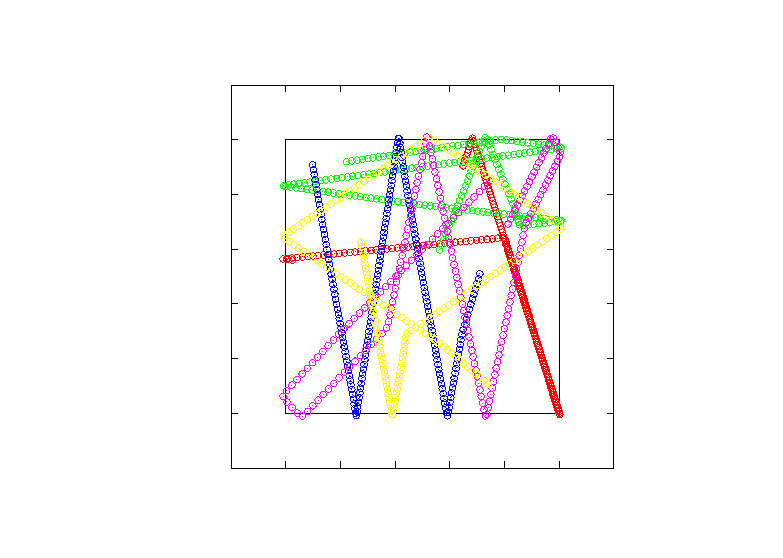
\includegraphics{../Report/figures/P_005_005}}%
    \gplfronttext
  \end{picture}%
\endgroup
}
				\caption{Path of five particles, with collisions}
			\end{subfigure}
			\begin{subfigure}{.45\textwidth}
				\scalebox{0.6}{% GNUPLOT: LaTeX picture with Postscript
\begingroup
  \makeatletter
  \providecommand\color[2][]{%
    \GenericError{(gnuplot) \space\space\space\@spaces}{%
      Package color not loaded in conjunction with
      terminal option `colourtext'%
    }{See the gnuplot documentation for explanation.%
    }{Either use 'blacktext' in gnuplot or load the package
      color.sty in LaTeX.}%
    \renewcommand\color[2][]{}%
  }%
  \providecommand\includegraphics[2][]{%
    \GenericError{(gnuplot) \space\space\space\@spaces}{%
      Package graphicx or graphics not loaded%
    }{See the gnuplot documentation for explanation.%
    }{The gnuplot epslatex terminal needs graphicx.sty or graphics.sty.}%
    \renewcommand\includegraphics[2][]{}%
  }%
  \providecommand\rotatebox[2]{#2}%
  \@ifundefined{ifGPcolor}{%
    \newif\ifGPcolor
    \GPcolortrue
  }{}%
  \@ifundefined{ifGPblacktext}{%
    \newif\ifGPblacktext
    \GPblacktexttrue
  }{}%
  % define a \g@addto@macro without @ in the name:
  \let\gplgaddtomacro\g@addto@macro
  % define empty templates for all commands taking text:
  \gdef\gplbacktext{}%
  \gdef\gplfronttext{}%
  \makeatother
  \ifGPblacktext
    % no textcolor at all
    \def\colorrgb#1{}%
    \def\colorgray#1{}%
  \else
    % gray or color?
    \ifGPcolor
      \def\colorrgb#1{\color[rgb]{#1}}%
      \def\colorgray#1{\color[gray]{#1}}%
      \expandafter\def\csname LTw\endcsname{\color{white}}%
      \expandafter\def\csname LTb\endcsname{\color{black}}%
      \expandafter\def\csname LTa\endcsname{\color{black}}%
      \expandafter\def\csname LT0\endcsname{\color[rgb]{1,0,0}}%
      \expandafter\def\csname LT1\endcsname{\color[rgb]{0,1,0}}%
      \expandafter\def\csname LT2\endcsname{\color[rgb]{0,0,1}}%
      \expandafter\def\csname LT3\endcsname{\color[rgb]{1,0,1}}%
      \expandafter\def\csname LT4\endcsname{\color[rgb]{0,1,1}}%
      \expandafter\def\csname LT5\endcsname{\color[rgb]{1,1,0}}%
      \expandafter\def\csname LT6\endcsname{\color[rgb]{0,0,0}}%
      \expandafter\def\csname LT7\endcsname{\color[rgb]{1,0.3,0}}%
      \expandafter\def\csname LT8\endcsname{\color[rgb]{0.5,0.5,0.5}}%
    \else
      % gray
      \def\colorrgb#1{\color{black}}%
      \def\colorgray#1{\color[gray]{#1}}%
      \expandafter\def\csname LTw\endcsname{\color{white}}%
      \expandafter\def\csname LTb\endcsname{\color{black}}%
      \expandafter\def\csname LTa\endcsname{\color{black}}%
      \expandafter\def\csname LT0\endcsname{\color{black}}%
      \expandafter\def\csname LT1\endcsname{\color{black}}%
      \expandafter\def\csname LT2\endcsname{\color{black}}%
      \expandafter\def\csname LT3\endcsname{\color{black}}%
      \expandafter\def\csname LT4\endcsname{\color{black}}%
      \expandafter\def\csname LT5\endcsname{\color{black}}%
      \expandafter\def\csname LT6\endcsname{\color{black}}%
      \expandafter\def\csname LT7\endcsname{\color{black}}%
      \expandafter\def\csname LT8\endcsname{\color{black}}%
    \fi
  \fi
    \setlength{\unitlength}{0.0500bp}%
    \ifx\gptboxheight\undefined%
      \newlength{\gptboxheight}%
      \newlength{\gptboxwidth}%
      \newsavebox{\gptboxtext}%
    \fi%
    \setlength{\fboxrule}{0.5pt}%
    \setlength{\fboxsep}{1pt}%
\begin{picture}(7200.00,5040.00)%
    \gplgaddtomacro\gplbacktext{%
      \csname LTb\endcsname%%
      \put(682,704){\makebox(0,0)[r]{\strut{}$0$}}%
      \put(682,1163){\makebox(0,0)[r]{\strut{}$5$}}%
      \put(682,1623){\makebox(0,0)[r]{\strut{}$10$}}%
      \put(682,2082){\makebox(0,0)[r]{\strut{}$15$}}%
      \put(682,2542){\makebox(0,0)[r]{\strut{}$20$}}%
      \put(682,3001){\makebox(0,0)[r]{\strut{}$25$}}%
      \put(682,3460){\makebox(0,0)[r]{\strut{}$30$}}%
      \put(682,3920){\makebox(0,0)[r]{\strut{}$35$}}%
      \put(682,4379){\makebox(0,0)[r]{\strut{}$40$}}%
      \put(814,484){\makebox(0,0){\strut{}$0$}}%
      \put(1413,484){\makebox(0,0){\strut{}$0.5$}}%
      \put(2012,484){\makebox(0,0){\strut{}$1$}}%
      \put(2611,484){\makebox(0,0){\strut{}$1.5$}}%
      \put(3210,484){\makebox(0,0){\strut{}$2$}}%
      \put(3809,484){\makebox(0,0){\strut{}$2.5$}}%
      \put(4407,484){\makebox(0,0){\strut{}$3$}}%
      \put(5006,484){\makebox(0,0){\strut{}$3.5$}}%
      \put(5605,484){\makebox(0,0){\strut{}$4$}}%
      \put(6204,484){\makebox(0,0){\strut{}$4.5$}}%
      \put(6803,484){\makebox(0,0){\strut{}$5$}}%
    }%
    \gplgaddtomacro\gplfronttext{%
      \csname LTb\endcsname%%
      \put(209,2541){\rotatebox{-270}{\makebox(0,0){\strut{}E}}}%
      \put(3808,154){\makebox(0,0){\strut{}T}}%
      \put(3808,4709){\makebox(0,0){\strut{}Total energy per particle of 5 particles}}%
      \csname LTb\endcsname%%
      \put(5816,4206){\makebox(0,0)[r]{\strut{}Energy}}%
    }%
    \gplbacktext
    \put(0,0){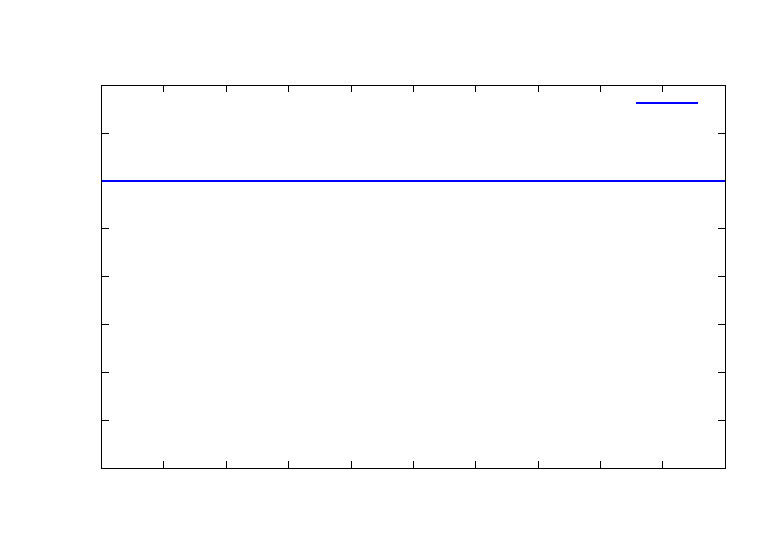
\includegraphics{../Report/figures/E_005_005}}%
    \gplfronttext
  \end{picture}%
\endgroup
}
				\caption{Total energy per particle of the five particles as the collisions happen}
			\end{subfigure}
			\caption{\label{five-collide}Five particles over a short time scale}
		\end{figure*}
		In figures \ref{two-collide}, \ref{three-collide}, \ref{four-collide} and \ref{five-collide} paths and energy drift as collisions happen is plotted. As we can see, the energy is very well conserved over short time spans. So we can pretty confidently expand the system. We now expand the box to $50\times50$ and the time to 200.
		
		\begin{figure*}[htb]
			\centering
			\begin{subfigure}{.45\textwidth}
				\hspace*{-2.6cm}\scalebox{0.9}{% GNUPLOT: LaTeX picture with Postscript
\begingroup
  % Encoding inside the plot.  In the header of your document, this encoding
  % should to defined, e.g., by using
  % \usepackage[cp1252,<other encodings>]{inputenc}
  \inputencoding{cp1252}%
  \makeatletter
  \providecommand\color[2][]{%
    \GenericError{(gnuplot) \space\space\space\@spaces}{%
      Package color not loaded in conjunction with
      terminal option `colourtext'%
    }{See the gnuplot documentation for explanation.%
    }{Either use 'blacktext' in gnuplot or load the package
      color.sty in LaTeX.}%
    \renewcommand\color[2][]{}%
  }%
  \providecommand\includegraphics[2][]{%
    \GenericError{(gnuplot) \space\space\space\@spaces}{%
      Package graphicx or graphics not loaded%
    }{See the gnuplot documentation for explanation.%
    }{The gnuplot epslatex terminal needs graphicx.sty or graphics.sty.}%
    \renewcommand\includegraphics[2][]{}%
  }%
  \providecommand\rotatebox[2]{#2}%
  \@ifundefined{ifGPcolor}{%
    \newif\ifGPcolor
    \GPcolortrue
  }{}%
  \@ifundefined{ifGPblacktext}{%
    \newif\ifGPblacktext
    \GPblacktexttrue
  }{}%
  % define a \g@addto@macro without @ in the name:
  \let\gplgaddtomacro\g@addto@macro
  % define empty templates for all commands taking text:
  \gdef\gplbacktext{}%
  \gdef\gplfronttext{}%
  \makeatother
  \ifGPblacktext
    % no textcolor at all
    \def\colorrgb#1{}%
    \def\colorgray#1{}%
  \else
    % gray or color?
    \ifGPcolor
      \def\colorrgb#1{\color[rgb]{#1}}%
      \def\colorgray#1{\color[gray]{#1}}%
      \expandafter\def\csname LTw\endcsname{\color{white}}%
      \expandafter\def\csname LTb\endcsname{\color{black}}%
      \expandafter\def\csname LTa\endcsname{\color{black}}%
      \expandafter\def\csname LT0\endcsname{\color[rgb]{1,0,0}}%
      \expandafter\def\csname LT1\endcsname{\color[rgb]{0,1,0}}%
      \expandafter\def\csname LT2\endcsname{\color[rgb]{0,0,1}}%
      \expandafter\def\csname LT3\endcsname{\color[rgb]{1,0,1}}%
      \expandafter\def\csname LT4\endcsname{\color[rgb]{0,1,1}}%
      \expandafter\def\csname LT5\endcsname{\color[rgb]{1,1,0}}%
      \expandafter\def\csname LT6\endcsname{\color[rgb]{0,0,0}}%
      \expandafter\def\csname LT7\endcsname{\color[rgb]{1,0.3,0}}%
      \expandafter\def\csname LT8\endcsname{\color[rgb]{0.5,0.5,0.5}}%
    \else
      % gray
      \def\colorrgb#1{\color{black}}%
      \def\colorgray#1{\color[gray]{#1}}%
      \expandafter\def\csname LTw\endcsname{\color{white}}%
      \expandafter\def\csname LTb\endcsname{\color{black}}%
      \expandafter\def\csname LTa\endcsname{\color{black}}%
      \expandafter\def\csname LT0\endcsname{\color{black}}%
      \expandafter\def\csname LT1\endcsname{\color{black}}%
      \expandafter\def\csname LT2\endcsname{\color{black}}%
      \expandafter\def\csname LT3\endcsname{\color{black}}%
      \expandafter\def\csname LT4\endcsname{\color{black}}%
      \expandafter\def\csname LT5\endcsname{\color{black}}%
      \expandafter\def\csname LT6\endcsname{\color{black}}%
      \expandafter\def\csname LT7\endcsname{\color{black}}%
      \expandafter\def\csname LT8\endcsname{\color{black}}%
    \fi
  \fi
    \setlength{\unitlength}{0.0500bp}%
    \ifx\gptboxheight\undefined%
      \newlength{\gptboxheight}%
      \newlength{\gptboxwidth}%
      \newsavebox{\gptboxtext}%
    \fi%
    \setlength{\fboxrule}{0.5pt}%
    \setlength{\fboxsep}{1pt}%
\begin{picture}(7200.00,5040.00)%
    \gplgaddtomacro\gplbacktext{%
      \csname LTb\endcsname%%
      \put(1927,840){\makebox(0,0)[r]{\strut{}$0$}}%
      \put(1927,1521){\makebox(0,0)[r]{\strut{}$10$}}%
      \put(1927,2201){\makebox(0,0)[r]{\strut{}$20$}}%
      \put(1927,2882){\makebox(0,0)[r]{\strut{}$30$}}%
      \put(1927,3562){\makebox(0,0)[r]{\strut{}$40$}}%
      \put(1927,4243){\makebox(0,0)[r]{\strut{}$50$}}%
      \put(2195,484){\makebox(0,0){\strut{}$0$}}%
      \put(2876,484){\makebox(0,0){\strut{}$10$}}%
      \put(3556,484){\makebox(0,0){\strut{}$20$}}%
      \put(4237,484){\makebox(0,0){\strut{}$30$}}%
      \put(4917,484){\makebox(0,0){\strut{}$40$}}%
      \put(5598,484){\makebox(0,0){\strut{}$50$}}%
    }%
    \gplgaddtomacro\gplfronttext{%
      \csname LTb\endcsname%%
      \put(1465,2541){\makebox(0,0){\strut{}y}}%
      \put(3896,154){\makebox(0,0){\strut{}x}}%
      \put(3896,4709){\makebox(0,0){\strut{}Trajectory of 1 particles in a system of 2 particles}}%
    }%
    \gplbacktext
    \put(0,0){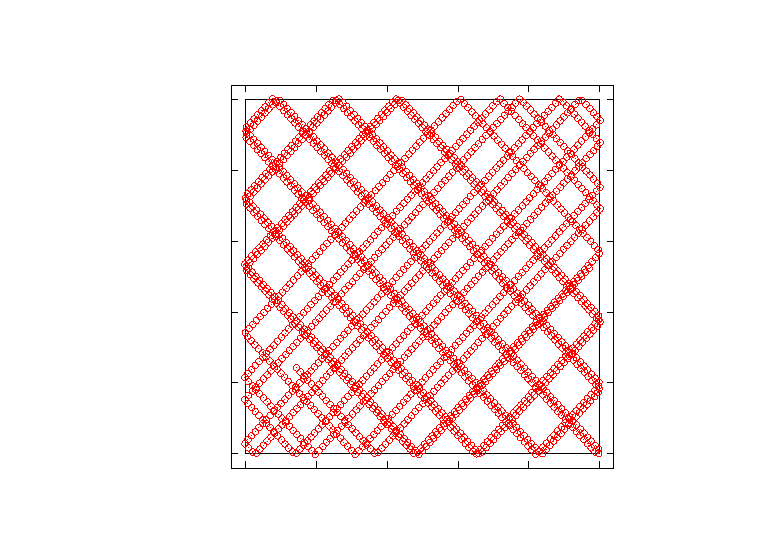
\includegraphics{../Report/figures/P_002_200}}%
    \gplfronttext
  \end{picture}%
\endgroup
}
				\caption{Path of one particle in a system with 2 particles}
			\end{subfigure}
			\begin{subfigure}{.45\textwidth}
				\hspace*{-2.6cm}\scalebox{0.9}{% GNUPLOT: LaTeX picture with Postscript
\begingroup
  % Encoding inside the plot.  In the header of your document, this encoding
  % should to defined, e.g., by using
  % \usepackage[cp1252,<other encodings>]{inputenc}
  \inputencoding{cp1252}%
  \makeatletter
  \providecommand\color[2][]{%
    \GenericError{(gnuplot) \space\space\space\@spaces}{%
      Package color not loaded in conjunction with
      terminal option `colourtext'%
    }{See the gnuplot documentation for explanation.%
    }{Either use 'blacktext' in gnuplot or load the package
      color.sty in LaTeX.}%
    \renewcommand\color[2][]{}%
  }%
  \providecommand\includegraphics[2][]{%
    \GenericError{(gnuplot) \space\space\space\@spaces}{%
      Package graphicx or graphics not loaded%
    }{See the gnuplot documentation for explanation.%
    }{The gnuplot epslatex terminal needs graphicx.sty or graphics.sty.}%
    \renewcommand\includegraphics[2][]{}%
  }%
  \providecommand\rotatebox[2]{#2}%
  \@ifundefined{ifGPcolor}{%
    \newif\ifGPcolor
    \GPcolortrue
  }{}%
  \@ifundefined{ifGPblacktext}{%
    \newif\ifGPblacktext
    \GPblacktexttrue
  }{}%
  % define a \g@addto@macro without @ in the name:
  \let\gplgaddtomacro\g@addto@macro
  % define empty templates for all commands taking text:
  \gdef\gplbacktext{}%
  \gdef\gplfronttext{}%
  \makeatother
  \ifGPblacktext
    % no textcolor at all
    \def\colorrgb#1{}%
    \def\colorgray#1{}%
  \else
    % gray or color?
    \ifGPcolor
      \def\colorrgb#1{\color[rgb]{#1}}%
      \def\colorgray#1{\color[gray]{#1}}%
      \expandafter\def\csname LTw\endcsname{\color{white}}%
      \expandafter\def\csname LTb\endcsname{\color{black}}%
      \expandafter\def\csname LTa\endcsname{\color{black}}%
      \expandafter\def\csname LT0\endcsname{\color[rgb]{1,0,0}}%
      \expandafter\def\csname LT1\endcsname{\color[rgb]{0,1,0}}%
      \expandafter\def\csname LT2\endcsname{\color[rgb]{0,0,1}}%
      \expandafter\def\csname LT3\endcsname{\color[rgb]{1,0,1}}%
      \expandafter\def\csname LT4\endcsname{\color[rgb]{0,1,1}}%
      \expandafter\def\csname LT5\endcsname{\color[rgb]{1,1,0}}%
      \expandafter\def\csname LT6\endcsname{\color[rgb]{0,0,0}}%
      \expandafter\def\csname LT7\endcsname{\color[rgb]{1,0.3,0}}%
      \expandafter\def\csname LT8\endcsname{\color[rgb]{0.5,0.5,0.5}}%
    \else
      % gray
      \def\colorrgb#1{\color{black}}%
      \def\colorgray#1{\color[gray]{#1}}%
      \expandafter\def\csname LTw\endcsname{\color{white}}%
      \expandafter\def\csname LTb\endcsname{\color{black}}%
      \expandafter\def\csname LTa\endcsname{\color{black}}%
      \expandafter\def\csname LT0\endcsname{\color{black}}%
      \expandafter\def\csname LT1\endcsname{\color{black}}%
      \expandafter\def\csname LT2\endcsname{\color{black}}%
      \expandafter\def\csname LT3\endcsname{\color{black}}%
      \expandafter\def\csname LT4\endcsname{\color{black}}%
      \expandafter\def\csname LT5\endcsname{\color{black}}%
      \expandafter\def\csname LT6\endcsname{\color{black}}%
      \expandafter\def\csname LT7\endcsname{\color{black}}%
      \expandafter\def\csname LT8\endcsname{\color{black}}%
    \fi
  \fi
    \setlength{\unitlength}{0.0500bp}%
    \ifx\gptboxheight\undefined%
      \newlength{\gptboxheight}%
      \newlength{\gptboxwidth}%
      \newsavebox{\gptboxtext}%
    \fi%
    \setlength{\fboxrule}{0.5pt}%
    \setlength{\fboxsep}{1pt}%
\begin{picture}(7200.00,5040.00)%
    \gplgaddtomacro\gplbacktext{%
      \csname LTb\endcsname%%
      \put(1927,840){\makebox(0,0)[r]{\strut{}$0$}}%
      \put(1927,1521){\makebox(0,0)[r]{\strut{}$10$}}%
      \put(1927,2201){\makebox(0,0)[r]{\strut{}$20$}}%
      \put(1927,2882){\makebox(0,0)[r]{\strut{}$30$}}%
      \put(1927,3562){\makebox(0,0)[r]{\strut{}$40$}}%
      \put(1927,4243){\makebox(0,0)[r]{\strut{}$50$}}%
      \put(2195,484){\makebox(0,0){\strut{}$0$}}%
      \put(2876,484){\makebox(0,0){\strut{}$10$}}%
      \put(3556,484){\makebox(0,0){\strut{}$20$}}%
      \put(4237,484){\makebox(0,0){\strut{}$30$}}%
      \put(4917,484){\makebox(0,0){\strut{}$40$}}%
      \put(5598,484){\makebox(0,0){\strut{}$50$}}%
    }%
    \gplgaddtomacro\gplfronttext{%
      \csname LTb\endcsname%%
      \put(1465,2541){\makebox(0,0){\strut{}y}}%
      \put(3896,154){\makebox(0,0){\strut{}x}}%
      \put(3896,4709){\makebox(0,0){\strut{}Trajectory of 1 particles in a system of 3 particles}}%
    }%
    \gplbacktext
    \put(0,0){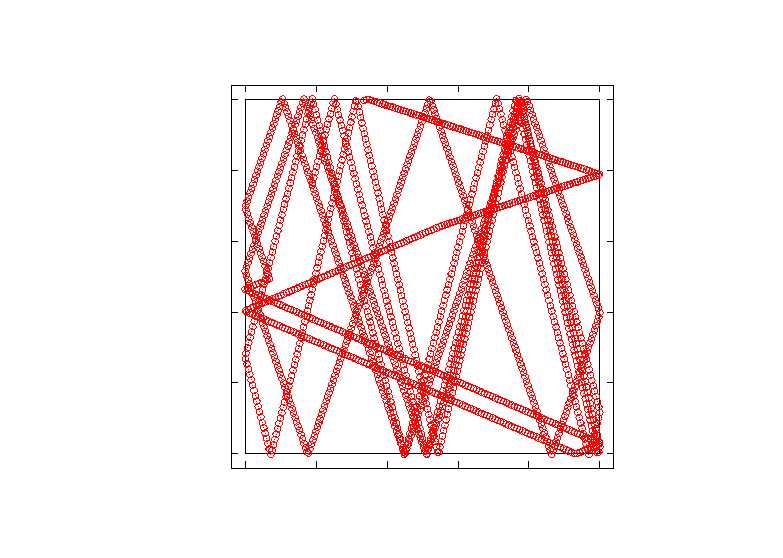
\includegraphics{../Report/figures/P_003_200}}%
    \gplfronttext
  \end{picture}%
\endgroup
}
				\caption{Path of one particle in a system with 3 particles}
			\end{subfigure}
			\begin{subfigure}{.45\textwidth}
				\hspace*{-2.6cm}\scalebox{0.9}{% GNUPLOT: LaTeX picture with Postscript
\begingroup
  % Encoding inside the plot.  In the header of your document, this encoding
  % should to defined, e.g., by using
  % \usepackage[cp1252,<other encodings>]{inputenc}
  \inputencoding{cp1252}%
  \makeatletter
  \providecommand\color[2][]{%
    \GenericError{(gnuplot) \space\space\space\@spaces}{%
      Package color not loaded in conjunction with
      terminal option `colourtext'%
    }{See the gnuplot documentation for explanation.%
    }{Either use 'blacktext' in gnuplot or load the package
      color.sty in LaTeX.}%
    \renewcommand\color[2][]{}%
  }%
  \providecommand\includegraphics[2][]{%
    \GenericError{(gnuplot) \space\space\space\@spaces}{%
      Package graphicx or graphics not loaded%
    }{See the gnuplot documentation for explanation.%
    }{The gnuplot epslatex terminal needs graphicx.sty or graphics.sty.}%
    \renewcommand\includegraphics[2][]{}%
  }%
  \providecommand\rotatebox[2]{#2}%
  \@ifundefined{ifGPcolor}{%
    \newif\ifGPcolor
    \GPcolortrue
  }{}%
  \@ifundefined{ifGPblacktext}{%
    \newif\ifGPblacktext
    \GPblacktexttrue
  }{}%
  % define a \g@addto@macro without @ in the name:
  \let\gplgaddtomacro\g@addto@macro
  % define empty templates for all commands taking text:
  \gdef\gplbacktext{}%
  \gdef\gplfronttext{}%
  \makeatother
  \ifGPblacktext
    % no textcolor at all
    \def\colorrgb#1{}%
    \def\colorgray#1{}%
  \else
    % gray or color?
    \ifGPcolor
      \def\colorrgb#1{\color[rgb]{#1}}%
      \def\colorgray#1{\color[gray]{#1}}%
      \expandafter\def\csname LTw\endcsname{\color{white}}%
      \expandafter\def\csname LTb\endcsname{\color{black}}%
      \expandafter\def\csname LTa\endcsname{\color{black}}%
      \expandafter\def\csname LT0\endcsname{\color[rgb]{1,0,0}}%
      \expandafter\def\csname LT1\endcsname{\color[rgb]{0,1,0}}%
      \expandafter\def\csname LT2\endcsname{\color[rgb]{0,0,1}}%
      \expandafter\def\csname LT3\endcsname{\color[rgb]{1,0,1}}%
      \expandafter\def\csname LT4\endcsname{\color[rgb]{0,1,1}}%
      \expandafter\def\csname LT5\endcsname{\color[rgb]{1,1,0}}%
      \expandafter\def\csname LT6\endcsname{\color[rgb]{0,0,0}}%
      \expandafter\def\csname LT7\endcsname{\color[rgb]{1,0.3,0}}%
      \expandafter\def\csname LT8\endcsname{\color[rgb]{0.5,0.5,0.5}}%
    \else
      % gray
      \def\colorrgb#1{\color{black}}%
      \def\colorgray#1{\color[gray]{#1}}%
      \expandafter\def\csname LTw\endcsname{\color{white}}%
      \expandafter\def\csname LTb\endcsname{\color{black}}%
      \expandafter\def\csname LTa\endcsname{\color{black}}%
      \expandafter\def\csname LT0\endcsname{\color{black}}%
      \expandafter\def\csname LT1\endcsname{\color{black}}%
      \expandafter\def\csname LT2\endcsname{\color{black}}%
      \expandafter\def\csname LT3\endcsname{\color{black}}%
      \expandafter\def\csname LT4\endcsname{\color{black}}%
      \expandafter\def\csname LT5\endcsname{\color{black}}%
      \expandafter\def\csname LT6\endcsname{\color{black}}%
      \expandafter\def\csname LT7\endcsname{\color{black}}%
      \expandafter\def\csname LT8\endcsname{\color{black}}%
    \fi
  \fi
    \setlength{\unitlength}{0.0500bp}%
    \ifx\gptboxheight\undefined%
      \newlength{\gptboxheight}%
      \newlength{\gptboxwidth}%
      \newsavebox{\gptboxtext}%
    \fi%
    \setlength{\fboxrule}{0.5pt}%
    \setlength{\fboxsep}{1pt}%
\begin{picture}(7200.00,5040.00)%
    \gplgaddtomacro\gplbacktext{%
      \csname LTb\endcsname%%
      \put(1927,840){\makebox(0,0)[r]{\strut{}$0$}}%
      \put(1927,1521){\makebox(0,0)[r]{\strut{}$10$}}%
      \put(1927,2201){\makebox(0,0)[r]{\strut{}$20$}}%
      \put(1927,2882){\makebox(0,0)[r]{\strut{}$30$}}%
      \put(1927,3562){\makebox(0,0)[r]{\strut{}$40$}}%
      \put(1927,4243){\makebox(0,0)[r]{\strut{}$50$}}%
      \put(2195,484){\makebox(0,0){\strut{}$0$}}%
      \put(2876,484){\makebox(0,0){\strut{}$10$}}%
      \put(3556,484){\makebox(0,0){\strut{}$20$}}%
      \put(4237,484){\makebox(0,0){\strut{}$30$}}%
      \put(4917,484){\makebox(0,0){\strut{}$40$}}%
      \put(5598,484){\makebox(0,0){\strut{}$50$}}%
    }%
    \gplgaddtomacro\gplfronttext{%
      \csname LTb\endcsname%%
      \put(1465,2541){\makebox(0,0){\strut{}y}}%
      \put(3896,154){\makebox(0,0){\strut{}x}}%
      \put(3896,4709){\makebox(0,0){\strut{}Trajectory of 1 particles in a system of 10 particles}}%
    }%
    \gplbacktext
    \put(0,0){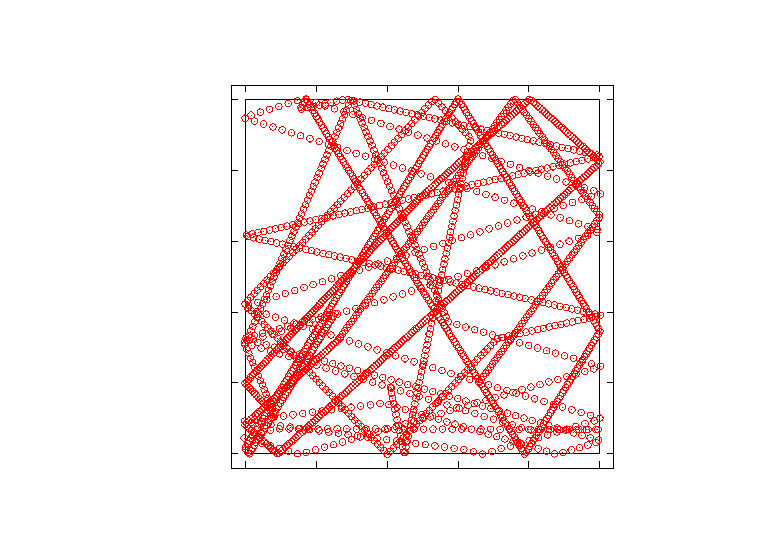
\includegraphics{../Report/figures/P_010_200}}%
    \gplfronttext
  \end{picture}%
\endgroup
}
				\caption{Path of one particle in a system with 10 particles}
			\end{subfigure}
			\begin{subfigure}{.45\textwidth}
				\hspace*{-2.6cm}\scalebox{0.9}{% GNUPLOT: LaTeX picture with Postscript
\begingroup
  % Encoding inside the plot.  In the header of your document, this encoding
  % should to defined, e.g., by using
  % \usepackage[cp1252,<other encodings>]{inputenc}
  \inputencoding{cp1252}%
  \makeatletter
  \providecommand\color[2][]{%
    \GenericError{(gnuplot) \space\space\space\@spaces}{%
      Package color not loaded in conjunction with
      terminal option `colourtext'%
    }{See the gnuplot documentation for explanation.%
    }{Either use 'blacktext' in gnuplot or load the package
      color.sty in LaTeX.}%
    \renewcommand\color[2][]{}%
  }%
  \providecommand\includegraphics[2][]{%
    \GenericError{(gnuplot) \space\space\space\@spaces}{%
      Package graphicx or graphics not loaded%
    }{See the gnuplot documentation for explanation.%
    }{The gnuplot epslatex terminal needs graphicx.sty or graphics.sty.}%
    \renewcommand\includegraphics[2][]{}%
  }%
  \providecommand\rotatebox[2]{#2}%
  \@ifundefined{ifGPcolor}{%
    \newif\ifGPcolor
    \GPcolortrue
  }{}%
  \@ifundefined{ifGPblacktext}{%
    \newif\ifGPblacktext
    \GPblacktexttrue
  }{}%
  % define a \g@addto@macro without @ in the name:
  \let\gplgaddtomacro\g@addto@macro
  % define empty templates for all commands taking text:
  \gdef\gplbacktext{}%
  \gdef\gplfronttext{}%
  \makeatother
  \ifGPblacktext
    % no textcolor at all
    \def\colorrgb#1{}%
    \def\colorgray#1{}%
  \else
    % gray or color?
    \ifGPcolor
      \def\colorrgb#1{\color[rgb]{#1}}%
      \def\colorgray#1{\color[gray]{#1}}%
      \expandafter\def\csname LTw\endcsname{\color{white}}%
      \expandafter\def\csname LTb\endcsname{\color{black}}%
      \expandafter\def\csname LTa\endcsname{\color{black}}%
      \expandafter\def\csname LT0\endcsname{\color[rgb]{1,0,0}}%
      \expandafter\def\csname LT1\endcsname{\color[rgb]{0,1,0}}%
      \expandafter\def\csname LT2\endcsname{\color[rgb]{0,0,1}}%
      \expandafter\def\csname LT3\endcsname{\color[rgb]{1,0,1}}%
      \expandafter\def\csname LT4\endcsname{\color[rgb]{0,1,1}}%
      \expandafter\def\csname LT5\endcsname{\color[rgb]{1,1,0}}%
      \expandafter\def\csname LT6\endcsname{\color[rgb]{0,0,0}}%
      \expandafter\def\csname LT7\endcsname{\color[rgb]{1,0.3,0}}%
      \expandafter\def\csname LT8\endcsname{\color[rgb]{0.5,0.5,0.5}}%
    \else
      % gray
      \def\colorrgb#1{\color{black}}%
      \def\colorgray#1{\color[gray]{#1}}%
      \expandafter\def\csname LTw\endcsname{\color{white}}%
      \expandafter\def\csname LTb\endcsname{\color{black}}%
      \expandafter\def\csname LTa\endcsname{\color{black}}%
      \expandafter\def\csname LT0\endcsname{\color{black}}%
      \expandafter\def\csname LT1\endcsname{\color{black}}%
      \expandafter\def\csname LT2\endcsname{\color{black}}%
      \expandafter\def\csname LT3\endcsname{\color{black}}%
      \expandafter\def\csname LT4\endcsname{\color{black}}%
      \expandafter\def\csname LT5\endcsname{\color{black}}%
      \expandafter\def\csname LT6\endcsname{\color{black}}%
      \expandafter\def\csname LT7\endcsname{\color{black}}%
      \expandafter\def\csname LT8\endcsname{\color{black}}%
    \fi
  \fi
    \setlength{\unitlength}{0.0500bp}%
    \ifx\gptboxheight\undefined%
      \newlength{\gptboxheight}%
      \newlength{\gptboxwidth}%
      \newsavebox{\gptboxtext}%
    \fi%
    \setlength{\fboxrule}{0.5pt}%
    \setlength{\fboxsep}{1pt}%
\begin{picture}(7200.00,5040.00)%
    \gplgaddtomacro\gplbacktext{%
      \csname LTb\endcsname%%
      \put(1927,840){\makebox(0,0)[r]{\strut{}$0$}}%
      \put(1927,1521){\makebox(0,0)[r]{\strut{}$10$}}%
      \put(1927,2201){\makebox(0,0)[r]{\strut{}$20$}}%
      \put(1927,2882){\makebox(0,0)[r]{\strut{}$30$}}%
      \put(1927,3562){\makebox(0,0)[r]{\strut{}$40$}}%
      \put(1927,4243){\makebox(0,0)[r]{\strut{}$50$}}%
      \put(2195,484){\makebox(0,0){\strut{}$0$}}%
      \put(2876,484){\makebox(0,0){\strut{}$10$}}%
      \put(3556,484){\makebox(0,0){\strut{}$20$}}%
      \put(4237,484){\makebox(0,0){\strut{}$30$}}%
      \put(4917,484){\makebox(0,0){\strut{}$40$}}%
      \put(5598,484){\makebox(0,0){\strut{}$50$}}%
    }%
    \gplgaddtomacro\gplfronttext{%
      \csname LTb\endcsname%%
      \put(1465,2541){\makebox(0,0){\strut{}y}}%
      \put(3896,154){\makebox(0,0){\strut{}x}}%
      \put(3896,4709){\makebox(0,0){\strut{}Trajectory of 1 particles in a system of 10 particles}}%
    }%
    \gplbacktext
    \put(0,0){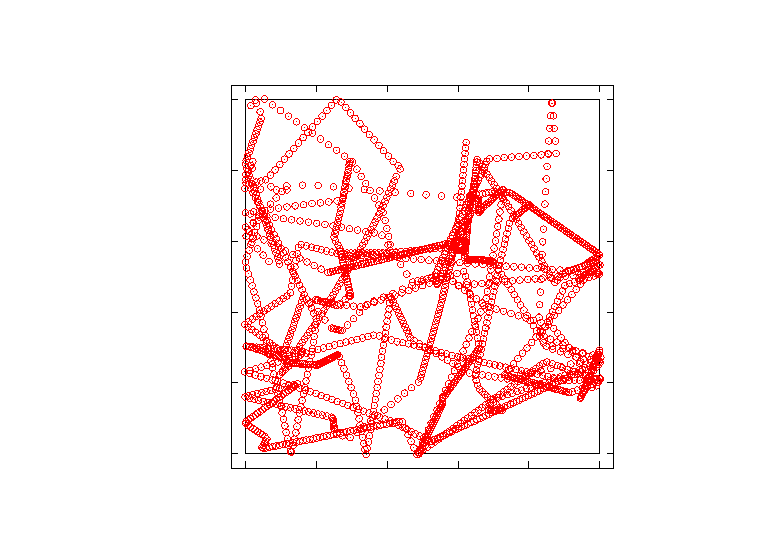
\includegraphics{../Report/figures/P_100_200}}%
    \gplfronttext
  \end{picture}%
\endgroup
}
				\caption{Path of one particle in a system with 100 particles}
			\end{subfigure}
			\caption{\label{path-one-in-large}Path of one particle in large system}
		\end{figure*}
		In figure \ref{path-one-in-large} the path of one particle is plotted as it explores the box. This might suggest that in gasses with low density the particles eventually explores all of the box. 
		
		In order to find out how the energy of the particles is distributed over time, all the energy might be given to a chosen number of particles by editing the "distr" parameter in the input file of the program. A system of $50\times50$ is chosen with 10 particles and the system is let go for a long time.
			
		\begin{figure*}[htb]
			\centering
			\begin{subfigure}{.45\textwidth}
				\scalebox{0.6}{% GNUPLOT: LaTeX picture with Postscript
\begingroup
  % Encoding inside the plot.  In the header of your document, this encoding
  % should to defined, e.g., by using
  % \usepackage[cp1252,<other encodings>]{inputenc}
  \inputencoding{cp1252}%
  \makeatletter
  \providecommand\color[2][]{%
    \GenericError{(gnuplot) \space\space\space\@spaces}{%
      Package color not loaded in conjunction with
      terminal option `colourtext'%
    }{See the gnuplot documentation for explanation.%
    }{Either use 'blacktext' in gnuplot or load the package
      color.sty in LaTeX.}%
    \renewcommand\color[2][]{}%
  }%
  \providecommand\includegraphics[2][]{%
    \GenericError{(gnuplot) \space\space\space\@spaces}{%
      Package graphicx or graphics not loaded%
    }{See the gnuplot documentation for explanation.%
    }{The gnuplot epslatex terminal needs graphicx.sty or graphics.sty.}%
    \renewcommand\includegraphics[2][]{}%
  }%
  \providecommand\rotatebox[2]{#2}%
  \@ifundefined{ifGPcolor}{%
    \newif\ifGPcolor
    \GPcolortrue
  }{}%
  \@ifundefined{ifGPblacktext}{%
    \newif\ifGPblacktext
    \GPblacktexttrue
  }{}%
  % define a \g@addto@macro without @ in the name:
  \let\gplgaddtomacro\g@addto@macro
  % define empty templates for all commands taking text:
  \gdef\gplbacktext{}%
  \gdef\gplfronttext{}%
  \makeatother
  \ifGPblacktext
    % no textcolor at all
    \def\colorrgb#1{}%
    \def\colorgray#1{}%
  \else
    % gray or color?
    \ifGPcolor
      \def\colorrgb#1{\color[rgb]{#1}}%
      \def\colorgray#1{\color[gray]{#1}}%
      \expandafter\def\csname LTw\endcsname{\color{white}}%
      \expandafter\def\csname LTb\endcsname{\color{black}}%
      \expandafter\def\csname LTa\endcsname{\color{black}}%
      \expandafter\def\csname LT0\endcsname{\color[rgb]{1,0,0}}%
      \expandafter\def\csname LT1\endcsname{\color[rgb]{0,1,0}}%
      \expandafter\def\csname LT2\endcsname{\color[rgb]{0,0,1}}%
      \expandafter\def\csname LT3\endcsname{\color[rgb]{1,0,1}}%
      \expandafter\def\csname LT4\endcsname{\color[rgb]{0,1,1}}%
      \expandafter\def\csname LT5\endcsname{\color[rgb]{1,1,0}}%
      \expandafter\def\csname LT6\endcsname{\color[rgb]{0,0,0}}%
      \expandafter\def\csname LT7\endcsname{\color[rgb]{1,0.3,0}}%
      \expandafter\def\csname LT8\endcsname{\color[rgb]{0.5,0.5,0.5}}%
    \else
      % gray
      \def\colorrgb#1{\color{black}}%
      \def\colorgray#1{\color[gray]{#1}}%
      \expandafter\def\csname LTw\endcsname{\color{white}}%
      \expandafter\def\csname LTb\endcsname{\color{black}}%
      \expandafter\def\csname LTa\endcsname{\color{black}}%
      \expandafter\def\csname LT0\endcsname{\color{black}}%
      \expandafter\def\csname LT1\endcsname{\color{black}}%
      \expandafter\def\csname LT2\endcsname{\color{black}}%
      \expandafter\def\csname LT3\endcsname{\color{black}}%
      \expandafter\def\csname LT4\endcsname{\color{black}}%
      \expandafter\def\csname LT5\endcsname{\color{black}}%
      \expandafter\def\csname LT6\endcsname{\color{black}}%
      \expandafter\def\csname LT7\endcsname{\color{black}}%
      \expandafter\def\csname LT8\endcsname{\color{black}}%
    \fi
  \fi
    \setlength{\unitlength}{0.0500bp}%
    \ifx\gptboxheight\undefined%
      \newlength{\gptboxheight}%
      \newlength{\gptboxwidth}%
      \newsavebox{\gptboxtext}%
    \fi%
    \setlength{\fboxrule}{0.5pt}%
    \setlength{\fboxsep}{1pt}%
\begin{picture}(7200.00,5040.00)%
    \gplgaddtomacro\gplbacktext{%
      \csname LTb\endcsname%%
      \put(858,704){\makebox(0,0)[r]{\strut{}$0$}}%
      \put(858,1439){\makebox(0,0)[r]{\strut{}$10$}}%
      \put(858,2174){\makebox(0,0)[r]{\strut{}$20$}}%
      \put(858,2909){\makebox(0,0)[r]{\strut{}$30$}}%
      \put(858,3644){\makebox(0,0)[r]{\strut{}$40$}}%
      \put(858,4379){\makebox(0,0)[r]{\strut{}$50$}}%
      \put(990,484){\makebox(0,0){\strut{}$0$}}%
      \put(1509,484){\makebox(0,0){\strut{}$1$}}%
      \put(2028,484){\makebox(0,0){\strut{}$2$}}%
      \put(2547,484){\makebox(0,0){\strut{}$3$}}%
      \put(3066,484){\makebox(0,0){\strut{}$4$}}%
      \put(3585,484){\makebox(0,0){\strut{}$5$}}%
      \put(4104,484){\makebox(0,0){\strut{}$6$}}%
      \put(4623,484){\makebox(0,0){\strut{}$7$}}%
      \put(5142,484){\makebox(0,0){\strut{}$8$}}%
      \put(5661,484){\makebox(0,0){\strut{}$9$}}%
      \put(6180,484){\makebox(0,0){\strut{}$10$}}%
      \put(6699,484){\makebox(0,0){\strut{}$11$}}%
    }%
    \gplgaddtomacro\gplfronttext{%
      \csname LTb\endcsname%%
      \put(396,2541){\makebox(0,0){\strut{}E}}%
      \put(3896,154){\makebox(0,0){\strut{}Particle}}%
      \put(3896,4709){\makebox(0,0){\strut{}Time averaged kinetic energy of 10 particles}}%
      \csname LTb\endcsname%%
      \put(5816,4206){\makebox(0,0)[r]{\strut{}Initial}}%
      \csname LTb\endcsname%%
      \put(5816,3986){\makebox(0,0)[r]{\strut{}Time averaged}}%
    }%
    \gplbacktext
    \put(0,0){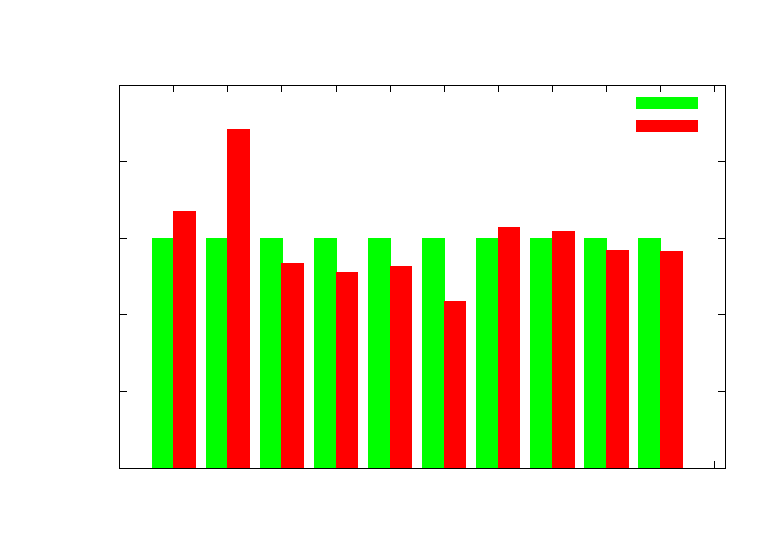
\includegraphics{../Report/figures/K_010_00}}%
    \gplfronttext
  \end{picture}%
\endgroup
}
				\caption{Kinetic energy for 10 particles at the start and the average kinetic energy with the energy evenly distributed at the start}
			\end{subfigure}
			\begin{subfigure}{.45\textwidth}
				\scalebox{0.6}{% GNUPLOT: LaTeX picture with Postscript
\begingroup
  % Encoding inside the plot.  In the header of your document, this encoding
  % should to defined, e.g., by using
  % \usepackage[cp1252,<other encodings>]{inputenc}
  \inputencoding{cp1252}%
  \makeatletter
  \providecommand\color[2][]{%
    \GenericError{(gnuplot) \space\space\space\@spaces}{%
      Package color not loaded in conjunction with
      terminal option `colourtext'%
    }{See the gnuplot documentation for explanation.%
    }{Either use 'blacktext' in gnuplot or load the package
      color.sty in LaTeX.}%
    \renewcommand\color[2][]{}%
  }%
  \providecommand\includegraphics[2][]{%
    \GenericError{(gnuplot) \space\space\space\@spaces}{%
      Package graphicx or graphics not loaded%
    }{See the gnuplot documentation for explanation.%
    }{The gnuplot epslatex terminal needs graphicx.sty or graphics.sty.}%
    \renewcommand\includegraphics[2][]{}%
  }%
  \providecommand\rotatebox[2]{#2}%
  \@ifundefined{ifGPcolor}{%
    \newif\ifGPcolor
    \GPcolortrue
  }{}%
  \@ifundefined{ifGPblacktext}{%
    \newif\ifGPblacktext
    \GPblacktexttrue
  }{}%
  % define a \g@addto@macro without @ in the name:
  \let\gplgaddtomacro\g@addto@macro
  % define empty templates for all commands taking text:
  \gdef\gplbacktext{}%
  \gdef\gplfronttext{}%
  \makeatother
  \ifGPblacktext
    % no textcolor at all
    \def\colorrgb#1{}%
    \def\colorgray#1{}%
  \else
    % gray or color?
    \ifGPcolor
      \def\colorrgb#1{\color[rgb]{#1}}%
      \def\colorgray#1{\color[gray]{#1}}%
      \expandafter\def\csname LTw\endcsname{\color{white}}%
      \expandafter\def\csname LTb\endcsname{\color{black}}%
      \expandafter\def\csname LTa\endcsname{\color{black}}%
      \expandafter\def\csname LT0\endcsname{\color[rgb]{1,0,0}}%
      \expandafter\def\csname LT1\endcsname{\color[rgb]{0,1,0}}%
      \expandafter\def\csname LT2\endcsname{\color[rgb]{0,0,1}}%
      \expandafter\def\csname LT3\endcsname{\color[rgb]{1,0,1}}%
      \expandafter\def\csname LT4\endcsname{\color[rgb]{0,1,1}}%
      \expandafter\def\csname LT5\endcsname{\color[rgb]{1,1,0}}%
      \expandafter\def\csname LT6\endcsname{\color[rgb]{0,0,0}}%
      \expandafter\def\csname LT7\endcsname{\color[rgb]{1,0.3,0}}%
      \expandafter\def\csname LT8\endcsname{\color[rgb]{0.5,0.5,0.5}}%
    \else
      % gray
      \def\colorrgb#1{\color{black}}%
      \def\colorgray#1{\color[gray]{#1}}%
      \expandafter\def\csname LTw\endcsname{\color{white}}%
      \expandafter\def\csname LTb\endcsname{\color{black}}%
      \expandafter\def\csname LTa\endcsname{\color{black}}%
      \expandafter\def\csname LT0\endcsname{\color{black}}%
      \expandafter\def\csname LT1\endcsname{\color{black}}%
      \expandafter\def\csname LT2\endcsname{\color{black}}%
      \expandafter\def\csname LT3\endcsname{\color{black}}%
      \expandafter\def\csname LT4\endcsname{\color{black}}%
      \expandafter\def\csname LT5\endcsname{\color{black}}%
      \expandafter\def\csname LT6\endcsname{\color{black}}%
      \expandafter\def\csname LT7\endcsname{\color{black}}%
      \expandafter\def\csname LT8\endcsname{\color{black}}%
    \fi
  \fi
    \setlength{\unitlength}{0.0500bp}%
    \ifx\gptboxheight\undefined%
      \newlength{\gptboxheight}%
      \newlength{\gptboxwidth}%
      \newsavebox{\gptboxtext}%
    \fi%
    \setlength{\fboxrule}{0.5pt}%
    \setlength{\fboxsep}{1pt}%
\begin{picture}(7200.00,5040.00)%
    \gplgaddtomacro\gplbacktext{%
      \csname LTb\endcsname%%
      \put(990,704){\makebox(0,0)[r]{\strut{}$0$}}%
      \put(990,1229){\makebox(0,0)[r]{\strut{}$50$}}%
      \put(990,1754){\makebox(0,0)[r]{\strut{}$100$}}%
      \put(990,2279){\makebox(0,0)[r]{\strut{}$150$}}%
      \put(990,2804){\makebox(0,0)[r]{\strut{}$200$}}%
      \put(990,3329){\makebox(0,0)[r]{\strut{}$250$}}%
      \put(990,3854){\makebox(0,0)[r]{\strut{}$300$}}%
      \put(990,4379){\makebox(0,0)[r]{\strut{}$350$}}%
      \put(1122,484){\makebox(0,0){\strut{}$0$}}%
      \put(1629,484){\makebox(0,0){\strut{}$1$}}%
      \put(2136,484){\makebox(0,0){\strut{}$2$}}%
      \put(2644,484){\makebox(0,0){\strut{}$3$}}%
      \put(3151,484){\makebox(0,0){\strut{}$4$}}%
      \put(3658,484){\makebox(0,0){\strut{}$5$}}%
      \put(4165,484){\makebox(0,0){\strut{}$6$}}%
      \put(4673,484){\makebox(0,0){\strut{}$7$}}%
      \put(5180,484){\makebox(0,0){\strut{}$8$}}%
      \put(5687,484){\makebox(0,0){\strut{}$9$}}%
      \put(6194,484){\makebox(0,0){\strut{}$10$}}%
      \put(6702,484){\makebox(0,0){\strut{}$11$}}%
    }%
    \gplgaddtomacro\gplfronttext{%
      \csname LTb\endcsname%%
      \put(396,2541){\makebox(0,0){\strut{}E}}%
      \put(3962,154){\makebox(0,0){\strut{}Particle}}%
      \put(3962,4709){\makebox(0,0){\strut{}Time averaged kinetic energy of 10 particles}}%
      \csname LTb\endcsname%%
      \put(5816,4206){\makebox(0,0)[r]{\strut{}Initial}}%
      \csname LTb\endcsname%%
      \put(5816,3986){\makebox(0,0)[r]{\strut{}Time averaged}}%
    }%
    \gplbacktext
    \put(0,0){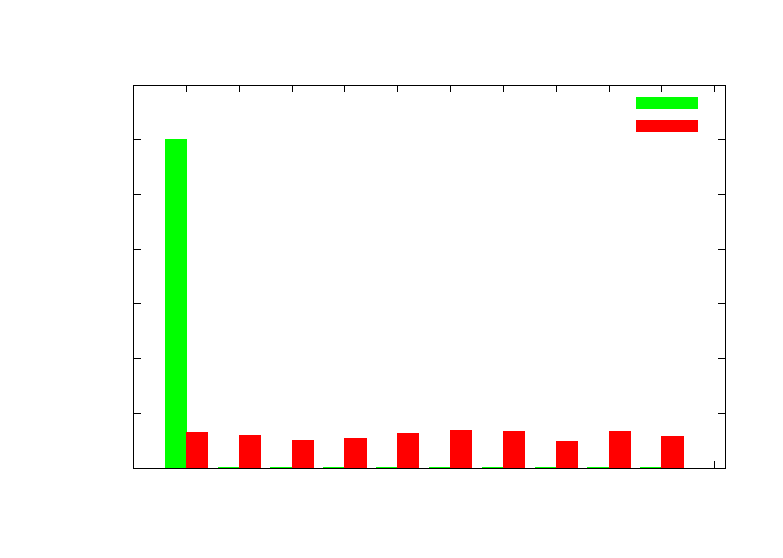
\includegraphics{../Report/figures/K_010_01}}%
    \gplfronttext
  \end{picture}%
\endgroup
}
				\caption{Kinetic energy for 10 particles at the start and the average kinetic energy with the all the energy given to one particle at the start}
			\end{subfigure}
			\begin{subfigure}{.45\textwidth}
				\scalebox{0.6}{% GNUPLOT: LaTeX picture with Postscript
\begingroup
  % Encoding inside the plot.  In the header of your document, this encoding
  % should to defined, e.g., by using
  % \usepackage[cp1252,<other encodings>]{inputenc}
  \inputencoding{cp1252}%
  \makeatletter
  \providecommand\color[2][]{%
    \GenericError{(gnuplot) \space\space\space\@spaces}{%
      Package color not loaded in conjunction with
      terminal option `colourtext'%
    }{See the gnuplot documentation for explanation.%
    }{Either use 'blacktext' in gnuplot or load the package
      color.sty in LaTeX.}%
    \renewcommand\color[2][]{}%
  }%
  \providecommand\includegraphics[2][]{%
    \GenericError{(gnuplot) \space\space\space\@spaces}{%
      Package graphicx or graphics not loaded%
    }{See the gnuplot documentation for explanation.%
    }{The gnuplot epslatex terminal needs graphicx.sty or graphics.sty.}%
    \renewcommand\includegraphics[2][]{}%
  }%
  \providecommand\rotatebox[2]{#2}%
  \@ifundefined{ifGPcolor}{%
    \newif\ifGPcolor
    \GPcolortrue
  }{}%
  \@ifundefined{ifGPblacktext}{%
    \newif\ifGPblacktext
    \GPblacktexttrue
  }{}%
  % define a \g@addto@macro without @ in the name:
  \let\gplgaddtomacro\g@addto@macro
  % define empty templates for all commands taking text:
  \gdef\gplbacktext{}%
  \gdef\gplfronttext{}%
  \makeatother
  \ifGPblacktext
    % no textcolor at all
    \def\colorrgb#1{}%
    \def\colorgray#1{}%
  \else
    % gray or color?
    \ifGPcolor
      \def\colorrgb#1{\color[rgb]{#1}}%
      \def\colorgray#1{\color[gray]{#1}}%
      \expandafter\def\csname LTw\endcsname{\color{white}}%
      \expandafter\def\csname LTb\endcsname{\color{black}}%
      \expandafter\def\csname LTa\endcsname{\color{black}}%
      \expandafter\def\csname LT0\endcsname{\color[rgb]{1,0,0}}%
      \expandafter\def\csname LT1\endcsname{\color[rgb]{0,1,0}}%
      \expandafter\def\csname LT2\endcsname{\color[rgb]{0,0,1}}%
      \expandafter\def\csname LT3\endcsname{\color[rgb]{1,0,1}}%
      \expandafter\def\csname LT4\endcsname{\color[rgb]{0,1,1}}%
      \expandafter\def\csname LT5\endcsname{\color[rgb]{1,1,0}}%
      \expandafter\def\csname LT6\endcsname{\color[rgb]{0,0,0}}%
      \expandafter\def\csname LT7\endcsname{\color[rgb]{1,0.3,0}}%
      \expandafter\def\csname LT8\endcsname{\color[rgb]{0.5,0.5,0.5}}%
    \else
      % gray
      \def\colorrgb#1{\color{black}}%
      \def\colorgray#1{\color[gray]{#1}}%
      \expandafter\def\csname LTw\endcsname{\color{white}}%
      \expandafter\def\csname LTb\endcsname{\color{black}}%
      \expandafter\def\csname LTa\endcsname{\color{black}}%
      \expandafter\def\csname LT0\endcsname{\color{black}}%
      \expandafter\def\csname LT1\endcsname{\color{black}}%
      \expandafter\def\csname LT2\endcsname{\color{black}}%
      \expandafter\def\csname LT3\endcsname{\color{black}}%
      \expandafter\def\csname LT4\endcsname{\color{black}}%
      \expandafter\def\csname LT5\endcsname{\color{black}}%
      \expandafter\def\csname LT6\endcsname{\color{black}}%
      \expandafter\def\csname LT7\endcsname{\color{black}}%
      \expandafter\def\csname LT8\endcsname{\color{black}}%
    \fi
  \fi
    \setlength{\unitlength}{0.0500bp}%
    \ifx\gptboxheight\undefined%
      \newlength{\gptboxheight}%
      \newlength{\gptboxwidth}%
      \newsavebox{\gptboxtext}%
    \fi%
    \setlength{\fboxrule}{0.5pt}%
    \setlength{\fboxsep}{1pt}%
\begin{picture}(7200.00,5040.00)%
    \gplgaddtomacro\gplbacktext{%
      \csname LTb\endcsname%%
      \put(990,704){\makebox(0,0)[r]{\strut{}$0$}}%
      \put(990,1194){\makebox(0,0)[r]{\strut{}$20$}}%
      \put(990,1684){\makebox(0,0)[r]{\strut{}$40$}}%
      \put(990,2174){\makebox(0,0)[r]{\strut{}$60$}}%
      \put(990,2664){\makebox(0,0)[r]{\strut{}$80$}}%
      \put(990,3154){\makebox(0,0)[r]{\strut{}$100$}}%
      \put(990,3644){\makebox(0,0)[r]{\strut{}$120$}}%
      \put(990,4134){\makebox(0,0)[r]{\strut{}$140$}}%
      \put(1122,484){\makebox(0,0){\strut{}$0$}}%
      \put(1629,484){\makebox(0,0){\strut{}$1$}}%
      \put(2136,484){\makebox(0,0){\strut{}$2$}}%
      \put(2644,484){\makebox(0,0){\strut{}$3$}}%
      \put(3151,484){\makebox(0,0){\strut{}$4$}}%
      \put(3658,484){\makebox(0,0){\strut{}$5$}}%
      \put(4165,484){\makebox(0,0){\strut{}$6$}}%
      \put(4673,484){\makebox(0,0){\strut{}$7$}}%
      \put(5180,484){\makebox(0,0){\strut{}$8$}}%
      \put(5687,484){\makebox(0,0){\strut{}$9$}}%
      \put(6194,484){\makebox(0,0){\strut{}$10$}}%
      \put(6702,484){\makebox(0,0){\strut{}$11$}}%
    }%
    \gplgaddtomacro\gplfronttext{%
      \csname LTb\endcsname%%
      \put(396,2541){\makebox(0,0){\strut{}E}}%
      \put(3962,154){\makebox(0,0){\strut{}Particle}}%
      \put(3962,4709){\makebox(0,0){\strut{}Time averaged kinetic energy of 10 particles}}%
      \csname LTb\endcsname%%
      \put(5816,4206){\makebox(0,0)[r]{\strut{}Initial}}%
      \csname LTb\endcsname%%
      \put(5816,3986){\makebox(0,0)[r]{\strut{}Time averaged}}%
    }%
    \gplbacktext
    \put(0,0){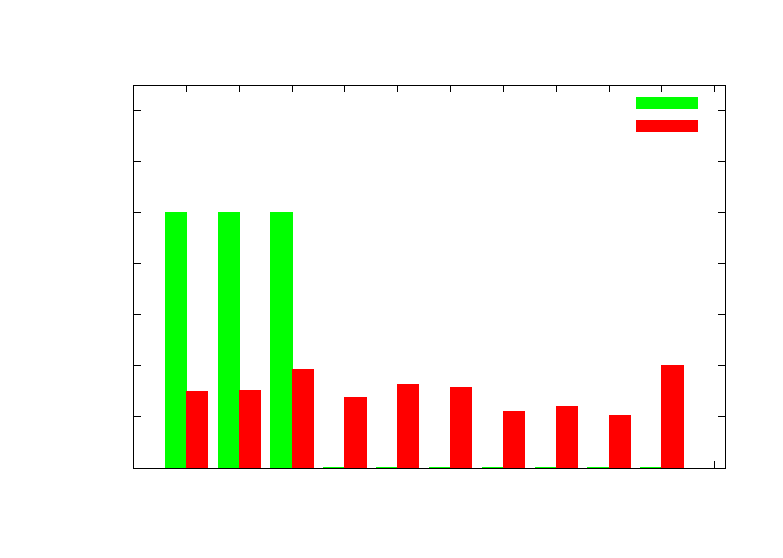
\includegraphics{../Report/figures/K_010_03}}%
    \gplfronttext
  \end{picture}%
\endgroup
}
				\caption{Kinetic energy for 10 particles at the start and the average kinetic energy with the energy evenly distributed among just 3 particles at the start}
			\end{subfigure}
			\caption{\label{energy-distr}Path of one particle with different values of time step $dt$}
		\end{figure*}
		in figure \ref{energy-distr} the energy is plotted as it is distributed among the particles, an animation of this can also be seen at \href{https://folk.ntnu.no/stiansjo/10_Particles_1_moving.gif}{this link} 
		
		In order to numerically calculate the probability distribution, 100 particles was simulated in a box with lengths 50 over a time of 1000 and an EPP of 10, larger EPP is unstable over very long times.
		\begin{figure*}
			\centering
			\scalebox{0.8}{% GNUPLOT: LaTeX picture with Postscript
\begingroup
  \makeatletter
  \providecommand\color[2][]{%
    \GenericError{(gnuplot) \space\space\space\@spaces}{%
      Package color not loaded in conjunction with
      terminal option `colourtext'%
    }{See the gnuplot documentation for explanation.%
    }{Either use 'blacktext' in gnuplot or load the package
      color.sty in LaTeX.}%
    \renewcommand\color[2][]{}%
  }%
  \providecommand\includegraphics[2][]{%
    \GenericError{(gnuplot) \space\space\space\@spaces}{%
      Package graphicx or graphics not loaded%
    }{See the gnuplot documentation for explanation.%
    }{The gnuplot epslatex terminal needs graphicx.sty or graphics.sty.}%
    \renewcommand\includegraphics[2][]{}%
  }%
  \providecommand\rotatebox[2]{#2}%
  \@ifundefined{ifGPcolor}{%
    \newif\ifGPcolor
    \GPcolortrue
  }{}%
  \@ifundefined{ifGPblacktext}{%
    \newif\ifGPblacktext
    \GPblacktexttrue
  }{}%
  % define a \g@addto@macro without @ in the name:
  \let\gplgaddtomacro\g@addto@macro
  % define empty templates for all commands taking text:
  \gdef\gplbacktext{}%
  \gdef\gplfronttext{}%
  \makeatother
  \ifGPblacktext
    % no textcolor at all
    \def\colorrgb#1{}%
    \def\colorgray#1{}%
  \else
    % gray or color?
    \ifGPcolor
      \def\colorrgb#1{\color[rgb]{#1}}%
      \def\colorgray#1{\color[gray]{#1}}%
      \expandafter\def\csname LTw\endcsname{\color{white}}%
      \expandafter\def\csname LTb\endcsname{\color{black}}%
      \expandafter\def\csname LTa\endcsname{\color{black}}%
      \expandafter\def\csname LT0\endcsname{\color[rgb]{1,0,0}}%
      \expandafter\def\csname LT1\endcsname{\color[rgb]{0,1,0}}%
      \expandafter\def\csname LT2\endcsname{\color[rgb]{0,0,1}}%
      \expandafter\def\csname LT3\endcsname{\color[rgb]{1,0,1}}%
      \expandafter\def\csname LT4\endcsname{\color[rgb]{0,1,1}}%
      \expandafter\def\csname LT5\endcsname{\color[rgb]{1,1,0}}%
      \expandafter\def\csname LT6\endcsname{\color[rgb]{0,0,0}}%
      \expandafter\def\csname LT7\endcsname{\color[rgb]{1,0.3,0}}%
      \expandafter\def\csname LT8\endcsname{\color[rgb]{0.5,0.5,0.5}}%
    \else
      % gray
      \def\colorrgb#1{\color{black}}%
      \def\colorgray#1{\color[gray]{#1}}%
      \expandafter\def\csname LTw\endcsname{\color{white}}%
      \expandafter\def\csname LTb\endcsname{\color{black}}%
      \expandafter\def\csname LTa\endcsname{\color{black}}%
      \expandafter\def\csname LT0\endcsname{\color{black}}%
      \expandafter\def\csname LT1\endcsname{\color{black}}%
      \expandafter\def\csname LT2\endcsname{\color{black}}%
      \expandafter\def\csname LT3\endcsname{\color{black}}%
      \expandafter\def\csname LT4\endcsname{\color{black}}%
      \expandafter\def\csname LT5\endcsname{\color{black}}%
      \expandafter\def\csname LT6\endcsname{\color{black}}%
      \expandafter\def\csname LT7\endcsname{\color{black}}%
      \expandafter\def\csname LT8\endcsname{\color{black}}%
    \fi
  \fi
    \setlength{\unitlength}{0.0500bp}%
    \ifx\gptboxheight\undefined%
      \newlength{\gptboxheight}%
      \newlength{\gptboxwidth}%
      \newsavebox{\gptboxtext}%
    \fi%
    \setlength{\fboxrule}{0.5pt}%
    \setlength{\fboxsep}{1pt}%
\begin{picture}(7200.00,5040.00)%
    \gplgaddtomacro\gplbacktext{%
      \csname LTb\endcsname%%
      \put(946,704){\makebox(0,0)[r]{\strut{}$0$}}%
      \put(946,1229){\makebox(0,0)[r]{\strut{}$0.02$}}%
      \put(946,1754){\makebox(0,0)[r]{\strut{}$0.04$}}%
      \put(946,2279){\makebox(0,0)[r]{\strut{}$0.06$}}%
      \put(946,2804){\makebox(0,0)[r]{\strut{}$0.08$}}%
      \put(946,3329){\makebox(0,0)[r]{\strut{}$0.1$}}%
      \put(946,3854){\makebox(0,0)[r]{\strut{}$0.12$}}%
      \put(946,4379){\makebox(0,0)[r]{\strut{}$0.14$}}%
      \put(1078,484){\makebox(0,0){\strut{}$-15$}}%
      \put(2032,484){\makebox(0,0){\strut{}$-10$}}%
      \put(2986,484){\makebox(0,0){\strut{}$-5$}}%
      \put(3941,484){\makebox(0,0){\strut{}$0$}}%
      \put(4895,484){\makebox(0,0){\strut{}$5$}}%
      \put(5849,484){\makebox(0,0){\strut{}$10$}}%
      \put(6803,484){\makebox(0,0){\strut{}$15$}}%
    }%
    \gplgaddtomacro\gplfronttext{%
      \csname LTb\endcsname%%
      \put(209,2541){\rotatebox{-270}{\makebox(0,0){\strut{}Probability}}}%
      \put(3940,154){\makebox(0,0){\strut{}$v_x$}}%
      \put(3940,4709){\makebox(0,0){\strut{}Maxwell Boltzmann}}%
      \csname LTb\endcsname%%
      \put(5816,4206){\makebox(0,0)[r]{\strut{}Numerical Values}}%
      \csname LTb\endcsname%%
      \put(5816,3986){\makebox(0,0)[r]{\strut{}Theoretical}}%
    }%
    \gplbacktext
    \put(0,0){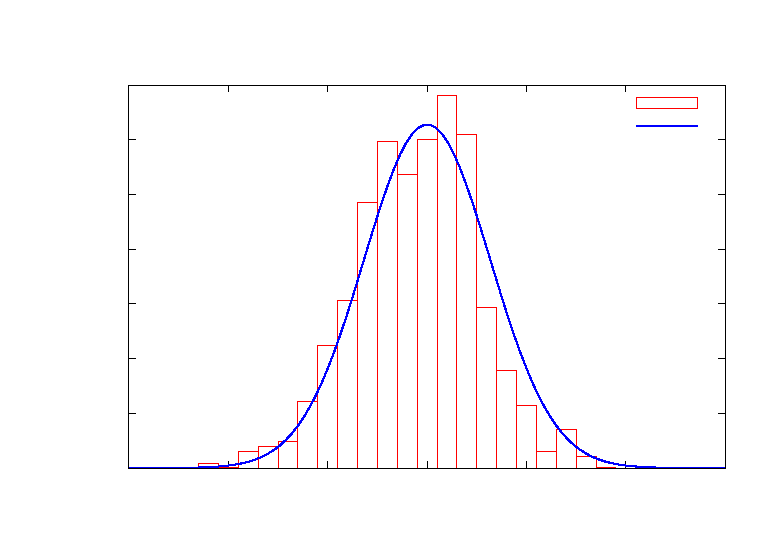
\includegraphics{../Report/figures/MB}}%
    \gplfronttext
  \end{picture}%
\endgroup
}
			\caption{\label{MB}Probability distribution of velocity of one particle}
		\end{figure*}
		In figure \ref{MB} the numerical and theoretical probability distributing is plotted for velocity in the x direction
		
		
	\section{Solids}
	We now want to explore how the system behaves when the kinetic energy is close to $\epsilon$ this is done by setting the EPP to around 1 and the hcp parameter to 1 to override most of the other parameters. The initial case is 19 particles in an hexagonal pattern.
	\begin{figure*}
		\centering
		\scalebox{0.7}{% GNUPLOT: LaTeX picture with Postscript
\begingroup
  % Encoding inside the plot.  In the header of your document, this encoding
  % should to defined, e.g., by using
  % \usepackage[cp1252,<other encodings>]{inputenc}
  \inputencoding{cp1252}%
  \makeatletter
  \providecommand\color[2][]{%
    \GenericError{(gnuplot) \space\space\space\@spaces}{%
      Package color not loaded in conjunction with
      terminal option `colourtext'%
    }{See the gnuplot documentation for explanation.%
    }{Either use 'blacktext' in gnuplot or load the package
      color.sty in LaTeX.}%
    \renewcommand\color[2][]{}%
  }%
  \providecommand\includegraphics[2][]{%
    \GenericError{(gnuplot) \space\space\space\@spaces}{%
      Package graphicx or graphics not loaded%
    }{See the gnuplot documentation for explanation.%
    }{The gnuplot epslatex terminal needs graphicx.sty or graphics.sty.}%
    \renewcommand\includegraphics[2][]{}%
  }%
  \providecommand\rotatebox[2]{#2}%
  \@ifundefined{ifGPcolor}{%
    \newif\ifGPcolor
    \GPcolortrue
  }{}%
  \@ifundefined{ifGPblacktext}{%
    \newif\ifGPblacktext
    \GPblacktexttrue
  }{}%
  % define a \g@addto@macro without @ in the name:
  \let\gplgaddtomacro\g@addto@macro
  % define empty templates for all commands taking text:
  \gdef\gplbacktext{}%
  \gdef\gplfronttext{}%
  \makeatother
  \ifGPblacktext
    % no textcolor at all
    \def\colorrgb#1{}%
    \def\colorgray#1{}%
  \else
    % gray or color?
    \ifGPcolor
      \def\colorrgb#1{\color[rgb]{#1}}%
      \def\colorgray#1{\color[gray]{#1}}%
      \expandafter\def\csname LTw\endcsname{\color{white}}%
      \expandafter\def\csname LTb\endcsname{\color{black}}%
      \expandafter\def\csname LTa\endcsname{\color{black}}%
      \expandafter\def\csname LT0\endcsname{\color[rgb]{1,0,0}}%
      \expandafter\def\csname LT1\endcsname{\color[rgb]{0,1,0}}%
      \expandafter\def\csname LT2\endcsname{\color[rgb]{0,0,1}}%
      \expandafter\def\csname LT3\endcsname{\color[rgb]{1,0,1}}%
      \expandafter\def\csname LT4\endcsname{\color[rgb]{0,1,1}}%
      \expandafter\def\csname LT5\endcsname{\color[rgb]{1,1,0}}%
      \expandafter\def\csname LT6\endcsname{\color[rgb]{0,0,0}}%
      \expandafter\def\csname LT7\endcsname{\color[rgb]{1,0.3,0}}%
      \expandafter\def\csname LT8\endcsname{\color[rgb]{0.5,0.5,0.5}}%
    \else
      % gray
      \def\colorrgb#1{\color{black}}%
      \def\colorgray#1{\color[gray]{#1}}%
      \expandafter\def\csname LTw\endcsname{\color{white}}%
      \expandafter\def\csname LTb\endcsname{\color{black}}%
      \expandafter\def\csname LTa\endcsname{\color{black}}%
      \expandafter\def\csname LT0\endcsname{\color{black}}%
      \expandafter\def\csname LT1\endcsname{\color{black}}%
      \expandafter\def\csname LT2\endcsname{\color{black}}%
      \expandafter\def\csname LT3\endcsname{\color{black}}%
      \expandafter\def\csname LT4\endcsname{\color{black}}%
      \expandafter\def\csname LT5\endcsname{\color{black}}%
      \expandafter\def\csname LT6\endcsname{\color{black}}%
      \expandafter\def\csname LT7\endcsname{\color{black}}%
      \expandafter\def\csname LT8\endcsname{\color{black}}%
    \fi
  \fi
    \setlength{\unitlength}{0.0500bp}%
    \ifx\gptboxheight\undefined%
      \newlength{\gptboxheight}%
      \newlength{\gptboxwidth}%
      \newsavebox{\gptboxtext}%
    \fi%
    \setlength{\fboxrule}{0.5pt}%
    \setlength{\fboxsep}{1pt}%
\begin{picture}(7200.00,5040.00)%
    \gplgaddtomacro\gplbacktext{%
      \csname LTb\endcsname%%
      \put(1927,704){\makebox(0,0)[r]{\strut{}$-2$}}%
      \csname LTb\endcsname%%
      \put(1927,967){\makebox(0,0)[r]{\strut{}$-1$}}%
      \csname LTb\endcsname%%
      \put(1927,1229){\makebox(0,0)[r]{\strut{}$0$}}%
      \csname LTb\endcsname%%
      \put(1927,1492){\makebox(0,0)[r]{\strut{}$1$}}%
      \csname LTb\endcsname%%
      \put(1927,1754){\makebox(0,0)[r]{\strut{}$2$}}%
      \csname LTb\endcsname%%
      \put(1927,2017){\makebox(0,0)[r]{\strut{}$3$}}%
      \csname LTb\endcsname%%
      \put(1927,2279){\makebox(0,0)[r]{\strut{}$4$}}%
      \csname LTb\endcsname%%
      \put(1927,2542){\makebox(0,0)[r]{\strut{}$5$}}%
      \csname LTb\endcsname%%
      \put(1927,2804){\makebox(0,0)[r]{\strut{}$6$}}%
      \csname LTb\endcsname%%
      \put(1927,3067){\makebox(0,0)[r]{\strut{}$7$}}%
      \csname LTb\endcsname%%
      \put(1927,3329){\makebox(0,0)[r]{\strut{}$8$}}%
      \csname LTb\endcsname%%
      \put(1927,3592){\makebox(0,0)[r]{\strut{}$9$}}%
      \csname LTb\endcsname%%
      \put(1927,3854){\makebox(0,0)[r]{\strut{}$10$}}%
      \csname LTb\endcsname%%
      \put(1927,4117){\makebox(0,0)[r]{\strut{}$11$}}%
      \csname LTb\endcsname%%
      \put(1927,4379){\makebox(0,0)[r]{\strut{}$12$}}%
      \csname LTb\endcsname%%
      \put(2059,484){\makebox(0,0){\strut{}$-2$}}%
      \csname LTb\endcsname%%
      \put(2322,484){\makebox(0,0){\strut{}$-1$}}%
      \csname LTb\endcsname%%
      \put(2584,484){\makebox(0,0){\strut{}$0$}}%
      \csname LTb\endcsname%%
      \put(2847,484){\makebox(0,0){\strut{}$1$}}%
      \csname LTb\endcsname%%
      \put(3109,484){\makebox(0,0){\strut{}$2$}}%
      \csname LTb\endcsname%%
      \put(3372,484){\makebox(0,0){\strut{}$3$}}%
      \csname LTb\endcsname%%
      \put(3634,484){\makebox(0,0){\strut{}$4$}}%
      \csname LTb\endcsname%%
      \put(3897,484){\makebox(0,0){\strut{}$5$}}%
      \csname LTb\endcsname%%
      \put(4159,484){\makebox(0,0){\strut{}$6$}}%
      \csname LTb\endcsname%%
      \put(4422,484){\makebox(0,0){\strut{}$7$}}%
      \csname LTb\endcsname%%
      \put(4684,484){\makebox(0,0){\strut{}$8$}}%
      \csname LTb\endcsname%%
      \put(4947,484){\makebox(0,0){\strut{}$9$}}%
      \csname LTb\endcsname%%
      \put(5209,484){\makebox(0,0){\strut{}$10$}}%
      \csname LTb\endcsname%%
      \put(5472,484){\makebox(0,0){\strut{}$11$}}%
      \csname LTb\endcsname%%
      \put(5734,484){\makebox(0,0){\strut{}$12$}}%
    }%
    \gplgaddtomacro\gplfronttext{%
      \csname LTb\endcsname%%
      \put(1465,2541){\makebox(0,0){\strut{}y}}%
      \put(3896,154){\makebox(0,0){\strut{}x}}%
      \put(3896,4709){\makebox(0,0){\strut{}Hexagonal packing}}%
    }%
    \gplbacktext
    \put(0,0){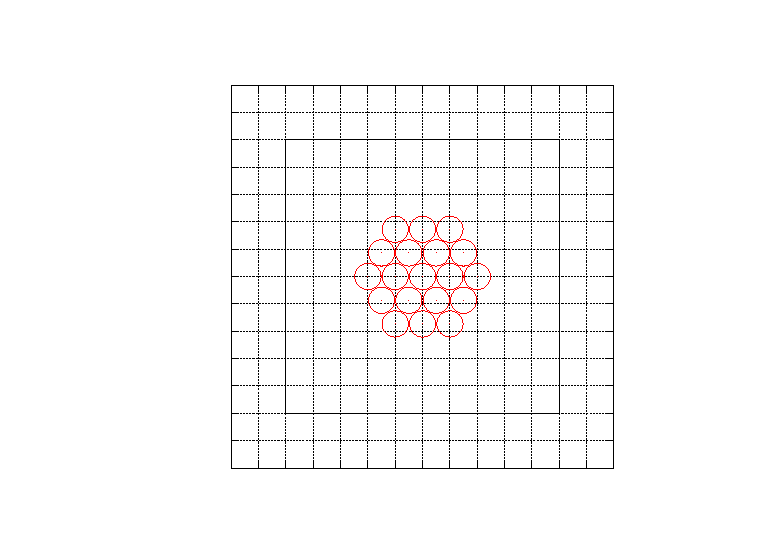
\includegraphics{../Report/figures/solidInit}}%
    \gplfronttext
  \end{picture}%
\endgroup
}
		\caption{\label{solid-init}The initial state of the solid, 19 particles packed in a hexagonal formation.}
	\end{figure*}
	The initial state is shown in figure \ref{solid-init}.
	\begin{figure*}[htb]
		\centering
		\begin{subfigure}{.45\textwidth}
			\hspace*{-2.6cm}\scalebox{0.9}{% GNUPLOT: LaTeX picture with Postscript
\begingroup
  % Encoding inside the plot.  In the header of your document, this encoding
  % should to defined, e.g., by using
  % \usepackage[cp1252,<other encodings>]{inputenc}
  \inputencoding{cp1252}%
  \makeatletter
  \providecommand\color[2][]{%
    \GenericError{(gnuplot) \space\space\space\@spaces}{%
      Package color not loaded in conjunction with
      terminal option `colourtext'%
    }{See the gnuplot documentation for explanation.%
    }{Either use 'blacktext' in gnuplot or load the package
      color.sty in LaTeX.}%
    \renewcommand\color[2][]{}%
  }%
  \providecommand\includegraphics[2][]{%
    \GenericError{(gnuplot) \space\space\space\@spaces}{%
      Package graphicx or graphics not loaded%
    }{See the gnuplot documentation for explanation.%
    }{The gnuplot epslatex terminal needs graphicx.sty or graphics.sty.}%
    \renewcommand\includegraphics[2][]{}%
  }%
  \providecommand\rotatebox[2]{#2}%
  \@ifundefined{ifGPcolor}{%
    \newif\ifGPcolor
    \GPcolortrue
  }{}%
  \@ifundefined{ifGPblacktext}{%
    \newif\ifGPblacktext
    \GPblacktexttrue
  }{}%
  % define a \g@addto@macro without @ in the name:
  \let\gplgaddtomacro\g@addto@macro
  % define empty templates for all commands taking text:
  \gdef\gplbacktext{}%
  \gdef\gplfronttext{}%
  \makeatother
  \ifGPblacktext
    % no textcolor at all
    \def\colorrgb#1{}%
    \def\colorgray#1{}%
  \else
    % gray or color?
    \ifGPcolor
      \def\colorrgb#1{\color[rgb]{#1}}%
      \def\colorgray#1{\color[gray]{#1}}%
      \expandafter\def\csname LTw\endcsname{\color{white}}%
      \expandafter\def\csname LTb\endcsname{\color{black}}%
      \expandafter\def\csname LTa\endcsname{\color{black}}%
      \expandafter\def\csname LT0\endcsname{\color[rgb]{1,0,0}}%
      \expandafter\def\csname LT1\endcsname{\color[rgb]{0,1,0}}%
      \expandafter\def\csname LT2\endcsname{\color[rgb]{0,0,1}}%
      \expandafter\def\csname LT3\endcsname{\color[rgb]{1,0,1}}%
      \expandafter\def\csname LT4\endcsname{\color[rgb]{0,1,1}}%
      \expandafter\def\csname LT5\endcsname{\color[rgb]{1,1,0}}%
      \expandafter\def\csname LT6\endcsname{\color[rgb]{0,0,0}}%
      \expandafter\def\csname LT7\endcsname{\color[rgb]{1,0.3,0}}%
      \expandafter\def\csname LT8\endcsname{\color[rgb]{0.5,0.5,0.5}}%
    \else
      % gray
      \def\colorrgb#1{\color{black}}%
      \def\colorgray#1{\color[gray]{#1}}%
      \expandafter\def\csname LTw\endcsname{\color{white}}%
      \expandafter\def\csname LTb\endcsname{\color{black}}%
      \expandafter\def\csname LTa\endcsname{\color{black}}%
      \expandafter\def\csname LT0\endcsname{\color{black}}%
      \expandafter\def\csname LT1\endcsname{\color{black}}%
      \expandafter\def\csname LT2\endcsname{\color{black}}%
      \expandafter\def\csname LT3\endcsname{\color{black}}%
      \expandafter\def\csname LT4\endcsname{\color{black}}%
      \expandafter\def\csname LT5\endcsname{\color{black}}%
      \expandafter\def\csname LT6\endcsname{\color{black}}%
      \expandafter\def\csname LT7\endcsname{\color{black}}%
      \expandafter\def\csname LT8\endcsname{\color{black}}%
    \fi
  \fi
    \setlength{\unitlength}{0.0500bp}%
    \ifx\gptboxheight\undefined%
      \newlength{\gptboxheight}%
      \newlength{\gptboxwidth}%
      \newsavebox{\gptboxtext}%
    \fi%
    \setlength{\fboxrule}{0.5pt}%
    \setlength{\fboxsep}{1pt}%
\begin{picture}(7200.00,5040.00)%
    \gplgaddtomacro\gplbacktext{%
      \csname LTb\endcsname%%
      \put(1927,704){\makebox(0,0)[r]{\strut{}$-2$}}%
      \csname LTb\endcsname%%
      \put(1927,967){\makebox(0,0)[r]{\strut{}$-1$}}%
      \csname LTb\endcsname%%
      \put(1927,1229){\makebox(0,0)[r]{\strut{}$0$}}%
      \csname LTb\endcsname%%
      \put(1927,1492){\makebox(0,0)[r]{\strut{}$1$}}%
      \csname LTb\endcsname%%
      \put(1927,1754){\makebox(0,0)[r]{\strut{}$2$}}%
      \csname LTb\endcsname%%
      \put(1927,2017){\makebox(0,0)[r]{\strut{}$3$}}%
      \csname LTb\endcsname%%
      \put(1927,2279){\makebox(0,0)[r]{\strut{}$4$}}%
      \csname LTb\endcsname%%
      \put(1927,2542){\makebox(0,0)[r]{\strut{}$5$}}%
      \csname LTb\endcsname%%
      \put(1927,2804){\makebox(0,0)[r]{\strut{}$6$}}%
      \csname LTb\endcsname%%
      \put(1927,3067){\makebox(0,0)[r]{\strut{}$7$}}%
      \csname LTb\endcsname%%
      \put(1927,3329){\makebox(0,0)[r]{\strut{}$8$}}%
      \csname LTb\endcsname%%
      \put(1927,3592){\makebox(0,0)[r]{\strut{}$9$}}%
      \csname LTb\endcsname%%
      \put(1927,3854){\makebox(0,0)[r]{\strut{}$10$}}%
      \csname LTb\endcsname%%
      \put(1927,4117){\makebox(0,0)[r]{\strut{}$11$}}%
      \csname LTb\endcsname%%
      \put(1927,4379){\makebox(0,0)[r]{\strut{}$12$}}%
      \csname LTb\endcsname%%
      \put(2059,484){\makebox(0,0){\strut{}$-2$}}%
      \csname LTb\endcsname%%
      \put(2322,484){\makebox(0,0){\strut{}$-1$}}%
      \csname LTb\endcsname%%
      \put(2584,484){\makebox(0,0){\strut{}$0$}}%
      \csname LTb\endcsname%%
      \put(2847,484){\makebox(0,0){\strut{}$1$}}%
      \csname LTb\endcsname%%
      \put(3109,484){\makebox(0,0){\strut{}$2$}}%
      \csname LTb\endcsname%%
      \put(3372,484){\makebox(0,0){\strut{}$3$}}%
      \csname LTb\endcsname%%
      \put(3634,484){\makebox(0,0){\strut{}$4$}}%
      \csname LTb\endcsname%%
      \put(3897,484){\makebox(0,0){\strut{}$5$}}%
      \csname LTb\endcsname%%
      \put(4159,484){\makebox(0,0){\strut{}$6$}}%
      \csname LTb\endcsname%%
      \put(4422,484){\makebox(0,0){\strut{}$7$}}%
      \csname LTb\endcsname%%
      \put(4684,484){\makebox(0,0){\strut{}$8$}}%
      \csname LTb\endcsname%%
      \put(4947,484){\makebox(0,0){\strut{}$9$}}%
      \csname LTb\endcsname%%
      \put(5209,484){\makebox(0,0){\strut{}$10$}}%
      \csname LTb\endcsname%%
      \put(5472,484){\makebox(0,0){\strut{}$11$}}%
      \csname LTb\endcsname%%
      \put(5734,484){\makebox(0,0){\strut{}$12$}}%
    }%
    \gplgaddtomacro\gplfronttext{%
      \csname LTb\endcsname%%
      \put(1465,2541){\makebox(0,0){\strut{}y}}%
      \put(3896,154){\makebox(0,0){\strut{}x}}%
      \put(3896,4709){\makebox(0,0){\strut{}Hexagonal packing}}%
    }%
    \gplbacktext
    \put(0,0){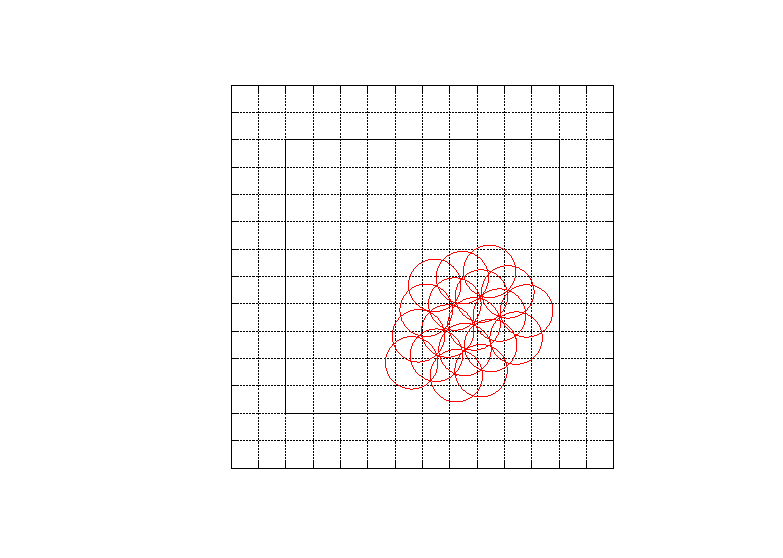
\includegraphics{../Report/figures/solid_end_05}}%
    \gplfronttext
  \end{picture}%
\endgroup
}
			\caption{The state of a solid after time evolution with an initial kinetic energy of 0.5}
		\end{subfigure}
		\begin{subfigure}{.45\textwidth}
			\hspace*{-2.6cm}\scalebox{0.9}{% GNUPLOT: LaTeX picture with Postscript
\begingroup
  % Encoding inside the plot.  In the header of your document, this encoding
  % should to defined, e.g., by using
  % \usepackage[cp1252,<other encodings>]{inputenc}
  \inputencoding{cp1252}%
  \makeatletter
  \providecommand\color[2][]{%
    \GenericError{(gnuplot) \space\space\space\@spaces}{%
      Package color not loaded in conjunction with
      terminal option `colourtext'%
    }{See the gnuplot documentation for explanation.%
    }{Either use 'blacktext' in gnuplot or load the package
      color.sty in LaTeX.}%
    \renewcommand\color[2][]{}%
  }%
  \providecommand\includegraphics[2][]{%
    \GenericError{(gnuplot) \space\space\space\@spaces}{%
      Package graphicx or graphics not loaded%
    }{See the gnuplot documentation for explanation.%
    }{The gnuplot epslatex terminal needs graphicx.sty or graphics.sty.}%
    \renewcommand\includegraphics[2][]{}%
  }%
  \providecommand\rotatebox[2]{#2}%
  \@ifundefined{ifGPcolor}{%
    \newif\ifGPcolor
    \GPcolortrue
  }{}%
  \@ifundefined{ifGPblacktext}{%
    \newif\ifGPblacktext
    \GPblacktexttrue
  }{}%
  % define a \g@addto@macro without @ in the name:
  \let\gplgaddtomacro\g@addto@macro
  % define empty templates for all commands taking text:
  \gdef\gplbacktext{}%
  \gdef\gplfronttext{}%
  \makeatother
  \ifGPblacktext
    % no textcolor at all
    \def\colorrgb#1{}%
    \def\colorgray#1{}%
  \else
    % gray or color?
    \ifGPcolor
      \def\colorrgb#1{\color[rgb]{#1}}%
      \def\colorgray#1{\color[gray]{#1}}%
      \expandafter\def\csname LTw\endcsname{\color{white}}%
      \expandafter\def\csname LTb\endcsname{\color{black}}%
      \expandafter\def\csname LTa\endcsname{\color{black}}%
      \expandafter\def\csname LT0\endcsname{\color[rgb]{1,0,0}}%
      \expandafter\def\csname LT1\endcsname{\color[rgb]{0,1,0}}%
      \expandafter\def\csname LT2\endcsname{\color[rgb]{0,0,1}}%
      \expandafter\def\csname LT3\endcsname{\color[rgb]{1,0,1}}%
      \expandafter\def\csname LT4\endcsname{\color[rgb]{0,1,1}}%
      \expandafter\def\csname LT5\endcsname{\color[rgb]{1,1,0}}%
      \expandafter\def\csname LT6\endcsname{\color[rgb]{0,0,0}}%
      \expandafter\def\csname LT7\endcsname{\color[rgb]{1,0.3,0}}%
      \expandafter\def\csname LT8\endcsname{\color[rgb]{0.5,0.5,0.5}}%
    \else
      % gray
      \def\colorrgb#1{\color{black}}%
      \def\colorgray#1{\color[gray]{#1}}%
      \expandafter\def\csname LTw\endcsname{\color{white}}%
      \expandafter\def\csname LTb\endcsname{\color{black}}%
      \expandafter\def\csname LTa\endcsname{\color{black}}%
      \expandafter\def\csname LT0\endcsname{\color{black}}%
      \expandafter\def\csname LT1\endcsname{\color{black}}%
      \expandafter\def\csname LT2\endcsname{\color{black}}%
      \expandafter\def\csname LT3\endcsname{\color{black}}%
      \expandafter\def\csname LT4\endcsname{\color{black}}%
      \expandafter\def\csname LT5\endcsname{\color{black}}%
      \expandafter\def\csname LT6\endcsname{\color{black}}%
      \expandafter\def\csname LT7\endcsname{\color{black}}%
      \expandafter\def\csname LT8\endcsname{\color{black}}%
    \fi
  \fi
    \setlength{\unitlength}{0.0500bp}%
    \ifx\gptboxheight\undefined%
      \newlength{\gptboxheight}%
      \newlength{\gptboxwidth}%
      \newsavebox{\gptboxtext}%
    \fi%
    \setlength{\fboxrule}{0.5pt}%
    \setlength{\fboxsep}{1pt}%
\begin{picture}(7200.00,5040.00)%
    \gplgaddtomacro\gplbacktext{%
      \csname LTb\endcsname%%
      \put(1927,704){\makebox(0,0)[r]{\strut{}$-2$}}%
      \csname LTb\endcsname%%
      \put(1927,967){\makebox(0,0)[r]{\strut{}$-1$}}%
      \csname LTb\endcsname%%
      \put(1927,1229){\makebox(0,0)[r]{\strut{}$0$}}%
      \csname LTb\endcsname%%
      \put(1927,1492){\makebox(0,0)[r]{\strut{}$1$}}%
      \csname LTb\endcsname%%
      \put(1927,1754){\makebox(0,0)[r]{\strut{}$2$}}%
      \csname LTb\endcsname%%
      \put(1927,2017){\makebox(0,0)[r]{\strut{}$3$}}%
      \csname LTb\endcsname%%
      \put(1927,2279){\makebox(0,0)[r]{\strut{}$4$}}%
      \csname LTb\endcsname%%
      \put(1927,2542){\makebox(0,0)[r]{\strut{}$5$}}%
      \csname LTb\endcsname%%
      \put(1927,2804){\makebox(0,0)[r]{\strut{}$6$}}%
      \csname LTb\endcsname%%
      \put(1927,3067){\makebox(0,0)[r]{\strut{}$7$}}%
      \csname LTb\endcsname%%
      \put(1927,3329){\makebox(0,0)[r]{\strut{}$8$}}%
      \csname LTb\endcsname%%
      \put(1927,3592){\makebox(0,0)[r]{\strut{}$9$}}%
      \csname LTb\endcsname%%
      \put(1927,3854){\makebox(0,0)[r]{\strut{}$10$}}%
      \csname LTb\endcsname%%
      \put(1927,4117){\makebox(0,0)[r]{\strut{}$11$}}%
      \csname LTb\endcsname%%
      \put(1927,4379){\makebox(0,0)[r]{\strut{}$12$}}%
      \csname LTb\endcsname%%
      \put(2059,484){\makebox(0,0){\strut{}$-2$}}%
      \csname LTb\endcsname%%
      \put(2322,484){\makebox(0,0){\strut{}$-1$}}%
      \csname LTb\endcsname%%
      \put(2584,484){\makebox(0,0){\strut{}$0$}}%
      \csname LTb\endcsname%%
      \put(2847,484){\makebox(0,0){\strut{}$1$}}%
      \csname LTb\endcsname%%
      \put(3109,484){\makebox(0,0){\strut{}$2$}}%
      \csname LTb\endcsname%%
      \put(3372,484){\makebox(0,0){\strut{}$3$}}%
      \csname LTb\endcsname%%
      \put(3634,484){\makebox(0,0){\strut{}$4$}}%
      \csname LTb\endcsname%%
      \put(3897,484){\makebox(0,0){\strut{}$5$}}%
      \csname LTb\endcsname%%
      \put(4159,484){\makebox(0,0){\strut{}$6$}}%
      \csname LTb\endcsname%%
      \put(4422,484){\makebox(0,0){\strut{}$7$}}%
      \csname LTb\endcsname%%
      \put(4684,484){\makebox(0,0){\strut{}$8$}}%
      \csname LTb\endcsname%%
      \put(4947,484){\makebox(0,0){\strut{}$9$}}%
      \csname LTb\endcsname%%
      \put(5209,484){\makebox(0,0){\strut{}$10$}}%
      \csname LTb\endcsname%%
      \put(5472,484){\makebox(0,0){\strut{}$11$}}%
      \csname LTb\endcsname%%
      \put(5734,484){\makebox(0,0){\strut{}$12$}}%
    }%
    \gplgaddtomacro\gplfronttext{%
      \csname LTb\endcsname%%
      \put(1465,2541){\makebox(0,0){\strut{}y}}%
      \put(3896,154){\makebox(0,0){\strut{}x}}%
      \put(3896,4709){\makebox(0,0){\strut{}Hexagonal packing}}%
    }%
    \gplbacktext
    \put(0,0){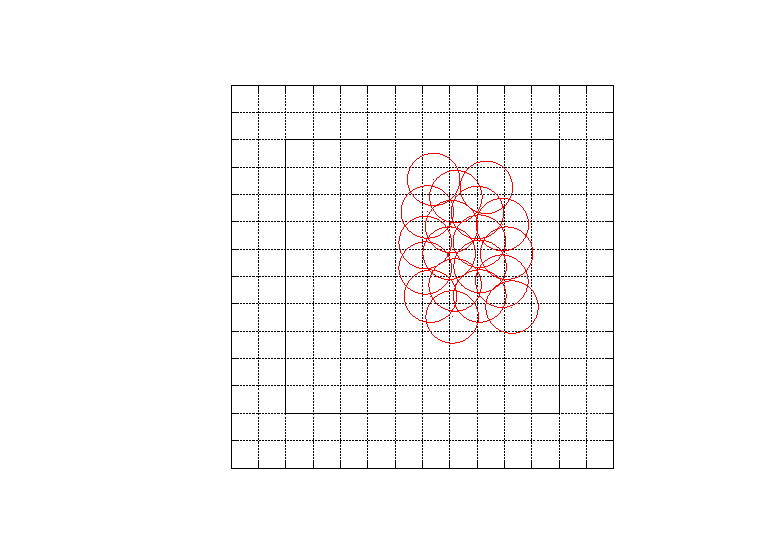
\includegraphics{../Report/figures/solid_end_10}}%
    \gplfronttext
  \end{picture}%
\endgroup
}
			\caption{The state of a solid after time evolution with an initial kinetic energy of 1.0}
		\end{subfigure}
		\begin{subfigure}{.45\textwidth}
			\hspace*{-2.6cm}\scalebox{0.9}{% GNUPLOT: LaTeX picture with Postscript
\begingroup
  % Encoding inside the plot.  In the header of your document, this encoding
  % should to defined, e.g., by using
  % \usepackage[cp1252,<other encodings>]{inputenc}
  \inputencoding{cp1252}%
  \makeatletter
  \providecommand\color[2][]{%
    \GenericError{(gnuplot) \space\space\space\@spaces}{%
      Package color not loaded in conjunction with
      terminal option `colourtext'%
    }{See the gnuplot documentation for explanation.%
    }{Either use 'blacktext' in gnuplot or load the package
      color.sty in LaTeX.}%
    \renewcommand\color[2][]{}%
  }%
  \providecommand\includegraphics[2][]{%
    \GenericError{(gnuplot) \space\space\space\@spaces}{%
      Package graphicx or graphics not loaded%
    }{See the gnuplot documentation for explanation.%
    }{The gnuplot epslatex terminal needs graphicx.sty or graphics.sty.}%
    \renewcommand\includegraphics[2][]{}%
  }%
  \providecommand\rotatebox[2]{#2}%
  \@ifundefined{ifGPcolor}{%
    \newif\ifGPcolor
    \GPcolortrue
  }{}%
  \@ifundefined{ifGPblacktext}{%
    \newif\ifGPblacktext
    \GPblacktexttrue
  }{}%
  % define a \g@addto@macro without @ in the name:
  \let\gplgaddtomacro\g@addto@macro
  % define empty templates for all commands taking text:
  \gdef\gplbacktext{}%
  \gdef\gplfronttext{}%
  \makeatother
  \ifGPblacktext
    % no textcolor at all
    \def\colorrgb#1{}%
    \def\colorgray#1{}%
  \else
    % gray or color?
    \ifGPcolor
      \def\colorrgb#1{\color[rgb]{#1}}%
      \def\colorgray#1{\color[gray]{#1}}%
      \expandafter\def\csname LTw\endcsname{\color{white}}%
      \expandafter\def\csname LTb\endcsname{\color{black}}%
      \expandafter\def\csname LTa\endcsname{\color{black}}%
      \expandafter\def\csname LT0\endcsname{\color[rgb]{1,0,0}}%
      \expandafter\def\csname LT1\endcsname{\color[rgb]{0,1,0}}%
      \expandafter\def\csname LT2\endcsname{\color[rgb]{0,0,1}}%
      \expandafter\def\csname LT3\endcsname{\color[rgb]{1,0,1}}%
      \expandafter\def\csname LT4\endcsname{\color[rgb]{0,1,1}}%
      \expandafter\def\csname LT5\endcsname{\color[rgb]{1,1,0}}%
      \expandafter\def\csname LT6\endcsname{\color[rgb]{0,0,0}}%
      \expandafter\def\csname LT7\endcsname{\color[rgb]{1,0.3,0}}%
      \expandafter\def\csname LT8\endcsname{\color[rgb]{0.5,0.5,0.5}}%
    \else
      % gray
      \def\colorrgb#1{\color{black}}%
      \def\colorgray#1{\color[gray]{#1}}%
      \expandafter\def\csname LTw\endcsname{\color{white}}%
      \expandafter\def\csname LTb\endcsname{\color{black}}%
      \expandafter\def\csname LTa\endcsname{\color{black}}%
      \expandafter\def\csname LT0\endcsname{\color{black}}%
      \expandafter\def\csname LT1\endcsname{\color{black}}%
      \expandafter\def\csname LT2\endcsname{\color{black}}%
      \expandafter\def\csname LT3\endcsname{\color{black}}%
      \expandafter\def\csname LT4\endcsname{\color{black}}%
      \expandafter\def\csname LT5\endcsname{\color{black}}%
      \expandafter\def\csname LT6\endcsname{\color{black}}%
      \expandafter\def\csname LT7\endcsname{\color{black}}%
      \expandafter\def\csname LT8\endcsname{\color{black}}%
    \fi
  \fi
    \setlength{\unitlength}{0.0500bp}%
    \ifx\gptboxheight\undefined%
      \newlength{\gptboxheight}%
      \newlength{\gptboxwidth}%
      \newsavebox{\gptboxtext}%
    \fi%
    \setlength{\fboxrule}{0.5pt}%
    \setlength{\fboxsep}{1pt}%
\begin{picture}(7200.00,5040.00)%
    \gplgaddtomacro\gplbacktext{%
      \csname LTb\endcsname%%
      \put(1927,704){\makebox(0,0)[r]{\strut{}$-2$}}%
      \csname LTb\endcsname%%
      \put(1927,967){\makebox(0,0)[r]{\strut{}$-1$}}%
      \csname LTb\endcsname%%
      \put(1927,1229){\makebox(0,0)[r]{\strut{}$0$}}%
      \csname LTb\endcsname%%
      \put(1927,1492){\makebox(0,0)[r]{\strut{}$1$}}%
      \csname LTb\endcsname%%
      \put(1927,1754){\makebox(0,0)[r]{\strut{}$2$}}%
      \csname LTb\endcsname%%
      \put(1927,2017){\makebox(0,0)[r]{\strut{}$3$}}%
      \csname LTb\endcsname%%
      \put(1927,2279){\makebox(0,0)[r]{\strut{}$4$}}%
      \csname LTb\endcsname%%
      \put(1927,2542){\makebox(0,0)[r]{\strut{}$5$}}%
      \csname LTb\endcsname%%
      \put(1927,2804){\makebox(0,0)[r]{\strut{}$6$}}%
      \csname LTb\endcsname%%
      \put(1927,3067){\makebox(0,0)[r]{\strut{}$7$}}%
      \csname LTb\endcsname%%
      \put(1927,3329){\makebox(0,0)[r]{\strut{}$8$}}%
      \csname LTb\endcsname%%
      \put(1927,3592){\makebox(0,0)[r]{\strut{}$9$}}%
      \csname LTb\endcsname%%
      \put(1927,3854){\makebox(0,0)[r]{\strut{}$10$}}%
      \csname LTb\endcsname%%
      \put(1927,4117){\makebox(0,0)[r]{\strut{}$11$}}%
      \csname LTb\endcsname%%
      \put(1927,4379){\makebox(0,0)[r]{\strut{}$12$}}%
      \csname LTb\endcsname%%
      \put(2059,484){\makebox(0,0){\strut{}$-2$}}%
      \csname LTb\endcsname%%
      \put(2322,484){\makebox(0,0){\strut{}$-1$}}%
      \csname LTb\endcsname%%
      \put(2584,484){\makebox(0,0){\strut{}$0$}}%
      \csname LTb\endcsname%%
      \put(2847,484){\makebox(0,0){\strut{}$1$}}%
      \csname LTb\endcsname%%
      \put(3109,484){\makebox(0,0){\strut{}$2$}}%
      \csname LTb\endcsname%%
      \put(3372,484){\makebox(0,0){\strut{}$3$}}%
      \csname LTb\endcsname%%
      \put(3634,484){\makebox(0,0){\strut{}$4$}}%
      \csname LTb\endcsname%%
      \put(3897,484){\makebox(0,0){\strut{}$5$}}%
      \csname LTb\endcsname%%
      \put(4159,484){\makebox(0,0){\strut{}$6$}}%
      \csname LTb\endcsname%%
      \put(4422,484){\makebox(0,0){\strut{}$7$}}%
      \csname LTb\endcsname%%
      \put(4684,484){\makebox(0,0){\strut{}$8$}}%
      \csname LTb\endcsname%%
      \put(4947,484){\makebox(0,0){\strut{}$9$}}%
      \csname LTb\endcsname%%
      \put(5209,484){\makebox(0,0){\strut{}$10$}}%
      \csname LTb\endcsname%%
      \put(5472,484){\makebox(0,0){\strut{}$11$}}%
      \csname LTb\endcsname%%
      \put(5734,484){\makebox(0,0){\strut{}$12$}}%
    }%
    \gplgaddtomacro\gplfronttext{%
      \csname LTb\endcsname%%
      \put(1465,2541){\makebox(0,0){\strut{}y}}%
      \put(3896,154){\makebox(0,0){\strut{}x}}%
      \put(3896,4709){\makebox(0,0){\strut{}Hexagonal packing}}%
    }%
    \gplbacktext
    \put(0,0){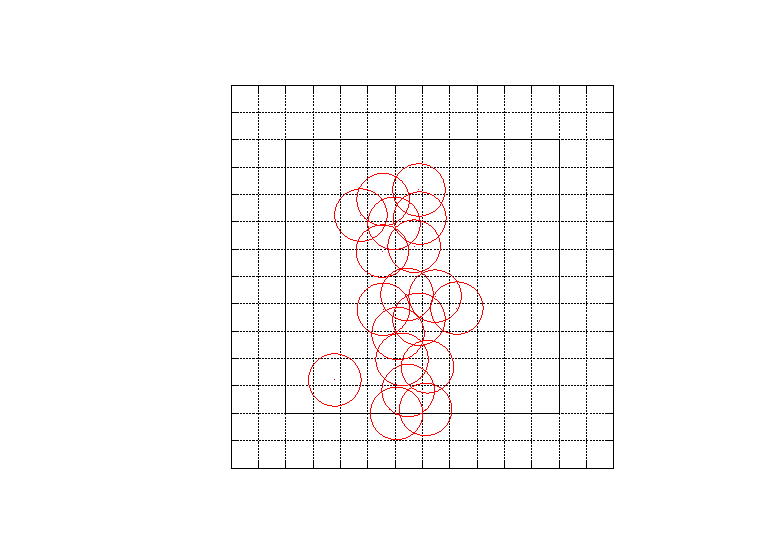
\includegraphics{../Report/figures/solid_end_20}}%
    \gplfronttext
  \end{picture}%
\endgroup
}
			\caption{The state of a solid after time evolution with an initial kinetic energy of 2.0}
		\end{subfigure}
		\begin{subfigure}{.45\textwidth}
			\hspace*{-2.6cm}\scalebox{0.9}{% GNUPLOT: LaTeX picture with Postscript
\begingroup
  % Encoding inside the plot.  In the header of your document, this encoding
  % should to defined, e.g., by using
  % \usepackage[cp1252,<other encodings>]{inputenc}
  \inputencoding{cp1252}%
  \makeatletter
  \providecommand\color[2][]{%
    \GenericError{(gnuplot) \space\space\space\@spaces}{%
      Package color not loaded in conjunction with
      terminal option `colourtext'%
    }{See the gnuplot documentation for explanation.%
    }{Either use 'blacktext' in gnuplot or load the package
      color.sty in LaTeX.}%
    \renewcommand\color[2][]{}%
  }%
  \providecommand\includegraphics[2][]{%
    \GenericError{(gnuplot) \space\space\space\@spaces}{%
      Package graphicx or graphics not loaded%
    }{See the gnuplot documentation for explanation.%
    }{The gnuplot epslatex terminal needs graphicx.sty or graphics.sty.}%
    \renewcommand\includegraphics[2][]{}%
  }%
  \providecommand\rotatebox[2]{#2}%
  \@ifundefined{ifGPcolor}{%
    \newif\ifGPcolor
    \GPcolortrue
  }{}%
  \@ifundefined{ifGPblacktext}{%
    \newif\ifGPblacktext
    \GPblacktexttrue
  }{}%
  % define a \g@addto@macro without @ in the name:
  \let\gplgaddtomacro\g@addto@macro
  % define empty templates for all commands taking text:
  \gdef\gplbacktext{}%
  \gdef\gplfronttext{}%
  \makeatother
  \ifGPblacktext
    % no textcolor at all
    \def\colorrgb#1{}%
    \def\colorgray#1{}%
  \else
    % gray or color?
    \ifGPcolor
      \def\colorrgb#1{\color[rgb]{#1}}%
      \def\colorgray#1{\color[gray]{#1}}%
      \expandafter\def\csname LTw\endcsname{\color{white}}%
      \expandafter\def\csname LTb\endcsname{\color{black}}%
      \expandafter\def\csname LTa\endcsname{\color{black}}%
      \expandafter\def\csname LT0\endcsname{\color[rgb]{1,0,0}}%
      \expandafter\def\csname LT1\endcsname{\color[rgb]{0,1,0}}%
      \expandafter\def\csname LT2\endcsname{\color[rgb]{0,0,1}}%
      \expandafter\def\csname LT3\endcsname{\color[rgb]{1,0,1}}%
      \expandafter\def\csname LT4\endcsname{\color[rgb]{0,1,1}}%
      \expandafter\def\csname LT5\endcsname{\color[rgb]{1,1,0}}%
      \expandafter\def\csname LT6\endcsname{\color[rgb]{0,0,0}}%
      \expandafter\def\csname LT7\endcsname{\color[rgb]{1,0.3,0}}%
      \expandafter\def\csname LT8\endcsname{\color[rgb]{0.5,0.5,0.5}}%
    \else
      % gray
      \def\colorrgb#1{\color{black}}%
      \def\colorgray#1{\color[gray]{#1}}%
      \expandafter\def\csname LTw\endcsname{\color{white}}%
      \expandafter\def\csname LTb\endcsname{\color{black}}%
      \expandafter\def\csname LTa\endcsname{\color{black}}%
      \expandafter\def\csname LT0\endcsname{\color{black}}%
      \expandafter\def\csname LT1\endcsname{\color{black}}%
      \expandafter\def\csname LT2\endcsname{\color{black}}%
      \expandafter\def\csname LT3\endcsname{\color{black}}%
      \expandafter\def\csname LT4\endcsname{\color{black}}%
      \expandafter\def\csname LT5\endcsname{\color{black}}%
      \expandafter\def\csname LT6\endcsname{\color{black}}%
      \expandafter\def\csname LT7\endcsname{\color{black}}%
      \expandafter\def\csname LT8\endcsname{\color{black}}%
    \fi
  \fi
    \setlength{\unitlength}{0.0500bp}%
    \ifx\gptboxheight\undefined%
      \newlength{\gptboxheight}%
      \newlength{\gptboxwidth}%
      \newsavebox{\gptboxtext}%
    \fi%
    \setlength{\fboxrule}{0.5pt}%
    \setlength{\fboxsep}{1pt}%
\begin{picture}(7200.00,5040.00)%
    \gplgaddtomacro\gplbacktext{%
      \csname LTb\endcsname%%
      \put(1927,704){\makebox(0,0)[r]{\strut{}$-2$}}%
      \csname LTb\endcsname%%
      \put(1927,967){\makebox(0,0)[r]{\strut{}$-1$}}%
      \csname LTb\endcsname%%
      \put(1927,1229){\makebox(0,0)[r]{\strut{}$0$}}%
      \csname LTb\endcsname%%
      \put(1927,1492){\makebox(0,0)[r]{\strut{}$1$}}%
      \csname LTb\endcsname%%
      \put(1927,1754){\makebox(0,0)[r]{\strut{}$2$}}%
      \csname LTb\endcsname%%
      \put(1927,2017){\makebox(0,0)[r]{\strut{}$3$}}%
      \csname LTb\endcsname%%
      \put(1927,2279){\makebox(0,0)[r]{\strut{}$4$}}%
      \csname LTb\endcsname%%
      \put(1927,2542){\makebox(0,0)[r]{\strut{}$5$}}%
      \csname LTb\endcsname%%
      \put(1927,2804){\makebox(0,0)[r]{\strut{}$6$}}%
      \csname LTb\endcsname%%
      \put(1927,3067){\makebox(0,0)[r]{\strut{}$7$}}%
      \csname LTb\endcsname%%
      \put(1927,3329){\makebox(0,0)[r]{\strut{}$8$}}%
      \csname LTb\endcsname%%
      \put(1927,3592){\makebox(0,0)[r]{\strut{}$9$}}%
      \csname LTb\endcsname%%
      \put(1927,3854){\makebox(0,0)[r]{\strut{}$10$}}%
      \csname LTb\endcsname%%
      \put(1927,4117){\makebox(0,0)[r]{\strut{}$11$}}%
      \csname LTb\endcsname%%
      \put(1927,4379){\makebox(0,0)[r]{\strut{}$12$}}%
      \csname LTb\endcsname%%
      \put(2059,484){\makebox(0,0){\strut{}$-2$}}%
      \csname LTb\endcsname%%
      \put(2322,484){\makebox(0,0){\strut{}$-1$}}%
      \csname LTb\endcsname%%
      \put(2584,484){\makebox(0,0){\strut{}$0$}}%
      \csname LTb\endcsname%%
      \put(2847,484){\makebox(0,0){\strut{}$1$}}%
      \csname LTb\endcsname%%
      \put(3109,484){\makebox(0,0){\strut{}$2$}}%
      \csname LTb\endcsname%%
      \put(3372,484){\makebox(0,0){\strut{}$3$}}%
      \csname LTb\endcsname%%
      \put(3634,484){\makebox(0,0){\strut{}$4$}}%
      \csname LTb\endcsname%%
      \put(3897,484){\makebox(0,0){\strut{}$5$}}%
      \csname LTb\endcsname%%
      \put(4159,484){\makebox(0,0){\strut{}$6$}}%
      \csname LTb\endcsname%%
      \put(4422,484){\makebox(0,0){\strut{}$7$}}%
      \csname LTb\endcsname%%
      \put(4684,484){\makebox(0,0){\strut{}$8$}}%
      \csname LTb\endcsname%%
      \put(4947,484){\makebox(0,0){\strut{}$9$}}%
      \csname LTb\endcsname%%
      \put(5209,484){\makebox(0,0){\strut{}$10$}}%
      \csname LTb\endcsname%%
      \put(5472,484){\makebox(0,0){\strut{}$11$}}%
      \csname LTb\endcsname%%
      \put(5734,484){\makebox(0,0){\strut{}$12$}}%
    }%
    \gplgaddtomacro\gplfronttext{%
      \csname LTb\endcsname%%
      \put(1465,2541){\makebox(0,0){\strut{}y}}%
      \put(3896,154){\makebox(0,0){\strut{}x}}%
      \put(3896,4709){\makebox(0,0){\strut{}Hexagonal packing}}%
    }%
    \gplbacktext
    \put(0,0){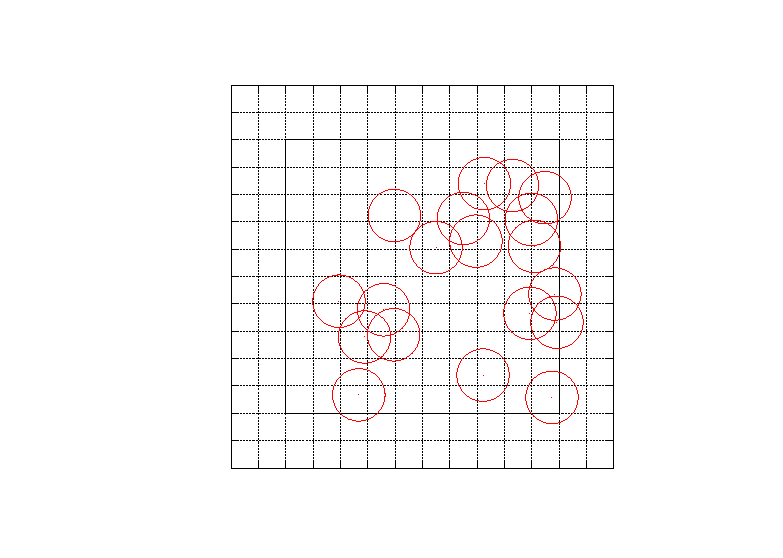
\includegraphics{../Report/figures/solid_end_24}}%
    \gplfronttext
  \end{picture}%
\endgroup
}
			\caption{\label{solid-24}The state of a solid after time evolution with an initial kinetic energy of 2.4}
		\end{subfigure}
		\caption{\label{solid-end}Path of one particle with different values of time step $dt$}
	\end{figure*}
	In figure \ref{solid-end} the end state with different initial energies i shown, in figure \ref{solid-24} the initial energy is chosen such that the total energy is around 0. 
	
	\begin{acknowledgments}
		The author would like to thank Mathilde Hirsum and Paul Gunnar Dommersnes for answering all questions raised during the implementation of the program.
	\end{acknowledgments}
	\appendix
	
		\section{Source code}
		
			The source code may have been given to you along with this text, if it wasnt the source code along with the source for this text and raw data can be found at \href{https://github.com/Mannen-I-Skogen/TFY4230-Numerical}{https://github.com/Mannen-I-Skogen/TFY4230-Numerical}
			
		\section{Animations}
		
			Some of the systems in this text are animated and can be found \href{https://folk.ntnu.no/stiansjo/particles}{Here}
	
	\bibliography{TFY4230-Statistical-Physics}

\end{document}